% \iffalse meta-comment
%
% Copyright (C) \the\year by Liu Benyuan <liubenyuan@gmail.com>
% This file may be distributed and/or modified under the
% conditions of the LaTeX Project Public License, either
% version 1.2 of this license or (at your option) any later
% version. The latest version of this license is in:
%
% http://www.latex-project.org/lppl.txt
%
% and version 1.2 or later is part of all distributions of
% LaTeX version 1999/12/01 or later.
%
% \fi
% 
% \iffalse
% <package>\NeedsTeXFormat{LaTeX2e}[1999/12/01]
% <package>\ProvidesPackage{nudtpaper}
% <package>		[2009/08/12 v1.0 By Liu Benyuan <liubenyuan@gmail.com>]
%<*driver>
\ProvidesFile{nudtpaper.dtx}[2009/08/12 v1.0 NUDT]
\documentclass[11pt]{ltxdoc}
\usepackage{nudtx}
\EnableCrossrefs
\CodelineIndex
\RecordChanges
\begin{document}
  \DocInput{\jobname.dtx}
\end{document}
%</driver>
% \fi
% 
% \def\thuthesis{\textsc{Thu}\-\textsc{Thesis}}
% \def\nudtpaper{\textsc{Nudt}\-\textsc{Paper}}
% 
% \CheckSum{1224}
% \CharacterTable
%  {Upper-case    \A\B\C\D\E\F\G\H\I\J\K\L\M\N\O\P\Q\R\S\T\U\V\W\X\Y\Z
%   Lower-case    \a\b\c\d\e\f\g\h\i\j\k\l\m\n\o\p\q\r\s\t\u\v\w\x\y\z
%   Digits        \0\1\2\3\4\5\6\7\8\9
%   Exclamation   \!     Double quote  \"     Hash (number) \#
%   Dollar        \$     Percent       \%     Ampersand     \&
%   Acute accent  \'     Left paren    \(     Right paren   \)
%   Asterisk      \*     Plus          \+     Comma         \,
%   Minus         \-     Point         \.     Solidus       \/
%   Colon         \:     Semicolon     \;     Less than     \<
%   Equals        \=     Greater than  \>     Question mark \?
%   Commercial at \@     Left bracket  \[     Backslash     \\
%   Right bracket \]     Circumflex    \^     Underscore    \_
%   Grave accent  \`     Left brace    \{     Vertical bar  \|
%   Right brace   \}     Tilde         \~}
%
% \changes{v0.99}{2009/08/12}{Initial Release}
%
% \GetFileInfo{\jobname.dtx}
% 
% \DoNotIndex{\begin,\end,\begingroup,\endgroup}
% \DoNotIndex{\ifx,\ifdim,\ifnum,\ifcase,\else,\or,\fi}
% \DoNotIndex{\let,\def,\xdef,\newcommand,\renewcommand}
% \DoNotIndex{\expandafter,\csname,\endcsname,\relax,\protect}
% \DoNotIndex{\Huge,\huge,\LARGE,\Large,\large,\normalsize}
% \DoNotIndex{\small,\footnotesize,\scriptsize,\tiny}
% \DoNotIndex{\normalfont,\bfseries,\slshape,\interlinepenalty}
% \DoNotIndex{\hfil,\par,\hskip,\vskip,\vspace,\quad}
% \DoNotIndex{\centering,\raggedright}
% \DoNotIndex{\c@secnumdepth,\@startsection,\@setfontsize}
% \DoNotIndex{\ ,\@plus,\@minus,\p@,\z@,\@m,\@M,\@ne,\m@ne}
% \DoNotIndex{\@@par,\DeclareOperation,\RequirePackage,\LoadClass}
% \DoNotIndex{\AtBeginDocument,\AtEndDocument}
%
% \IndexPrologue{\section*{索引}%
%    \addcontentsline{toc}{section}{索~~~~引}}
% \GlossaryPrologue{\section*{修改记录}%
%    \addcontentsline{toc}{section}{修改记录}}
%
% \renewcommand{\abstractname}{摘~~要}
% \renewcommand{\contentsname}{目~~录}
%
% \title{\textsc{NUDTpaper:}\,\,NUDT研究生学位论文\LaTeX{}模板使用手册\thanks{NUDT \LaTeX{} Thesis Template}}
% \author{刘本源 \\ \texttt{Liubenyuan@gmail.com}}
% \date{\fileversion\ (\filedate)}
%
% \maketitle
% \thispagestyle{empty}
%
% \begin{abstract}
% 本模板旨在提供规范的国防科学技术大学\LaTeX{}写作模板环境,
% 现支持硕士/博士学位论文格式,可以自动生成盲评、制作A3封面。
% \end{abstract}
%
% \vspace{2cm}
% \def\abstractname{免责声明}
% \begin{abstract}\noindent
% \begin{enumerate}
% \item 本模板的发布遵守 \LaTeX{} Project Public License,使用前请认真阅读协议内容
% \item 本模板创立参照官方严格的论文写作手册,并同时参照硕士/博士学位论文\textbf{doc}文档对比修改
% \item 国防科学技术大学对论文写作提供写作指南与官方\textbf{doc}模板,
% 同时提供官方的\LaTeX{}模板,本模板的出发点是方便大家使用专业的高效的论文书写工具,
% 其有点在于注重排版质量、命令规范、使用方便、更新及时,符合论文撰写说明。
% 但任何由于使用本模板而引起的论文格式审查问题均与本模板作者无关。
% \item 任何个人或组织均可以本模板为基础进行修改、扩展,生成新的专用模板,但请严格遵
% 守\LaTeX{} Project Public License 协议
% \item 欢迎提出修改意见
% \end{enumerate}
% \end{abstract}
%
% \clearpage
% \tableofcontents
%
% \clearpage
% \pagenumbering{arabic}
% \pagestyle{mainpage}
%
% \section{快速上手}
% 这部分是专门为那些想快速开始写论文的人准备的。
% \begin{description}
% \item[安装\TeX] 下载最新的\TeX{}live或者C\TeX{}并安装
% \item[字体] 用户需要具备\verb|simsun.ttf|, \verb|simhei.ttf|, \verb|simkai.ttf|,
% \verb|STZHONGS.TTF|, 上述字体都是windows自带的; 除此之外,在网上搜索(或者C\TeX{}
% 论坛)``Adobe Opentype 中文字体'',一搜一大把,确保下载下来Adobe的四款OTF字体:
% 宋,黑,仿宋,楷体。Linux用户可将上述字体复制到\verb|/usr/share/fonts/TTF|下。
% \item[试一试] 解压缩下载的模板,双击makepdf.bat(祈祷一下),如果生成了
% \verb|thesis.pdf|$\rightarrow$
% \item[那么我的那些常用的包都在么?] 你会想我的{\bf Trans}论文可以无缝
% 的复制过来么? 对于这一点,你可以修改\verb|mynudt.sty|来实现。但是{\hei 注意},大部分包
% 都在模板中了,而且{\hei 切记切记},不要擅自改动字体等版面设计,我们继续看$\rightarrow$
% \item[咦,数学公式不是很美观呀] 笔者{\hei 强烈}建议用户使用{\bf mtpro2}宏包的,怎么使用,
% 又有哪些好处,参见bookzh.sty吧!不会错的。好了,我们专注于内容本身吧$\rightarrow$
% \item[开始写了] 所有文件均采用UTF8编码,因此要保证你的\TeX{}编辑器
% (winedt, texworks, texmaker, vim, 记事本($\cdots{}$)等)支持这种编码,
% (经过一番搜索设置后)打开\verb|thesis.tex|,如果看到的是中文$\rightarrow$
% \item[漫长的写作] 手边准备着\LaTeX{}的常用帮助文档(数学,图表,引用等),
% 结合你喜欢的文献管理软件(JabRef等), 漫长的\texttt{编辑,编译,修改,编辑,
% 编译$\cdots$}过程之后,突然有一天发现你写完了$\rightarrow$
% \item[校订] 经过老师师兄师弟师妹齐心协力校正之后,你所做的只是:
% \texttt{生成明评论文,制作明评封面,生成盲评论文,制作盲评封面},
% 装订,上交$\rightarrow$
% \end{description}
% {\color{magenta} Done!}
%
% \section{模板介绍}
%
% \textsc{NUDTpaper} 旨在帮助并且推广\LaTeX{}在国防科技大学论文中的应用,
% 本文将尽可能帮助用户掌握\textsc{NUDTpaper}的安装方法,
% 如果仍旧有不清晰的地方可以参考样例文件或者
% 给作者邮件\footnote{liubenyuan@gmail.com},感兴趣的同学可以帮忙维护模板,
% 这个模板首先符合官方的设计要求,希望同学们在使用后能够提出你们的修改意见。
% 该模板很大程度上参考了6院黄老师sofoot的国防科大博士论文模板,
% 哈工大的\LaTeX{}模板以及清华的Thuthesis
% \footnote{主页:\url{http://thuthesis.sourceforge.net}},
% 有很多使用的帮助、\verb|.cls|中的命令以及版面设置均来自Thuthesis和sofoot的模板,
% 对此的引用表示感谢。
%
% {\color{blue}\fs 模板的作用在于减轻论文写作过程中格式调整的时间,
% 其前提就是遵守模板的用法,不提倡手动更改格式,不建议正文中使用
% 手动调节版面的命令,尤其禁止修改行距和使用\verb|\normalsize|,
% 否则即使使用了\textsc{NUDTpaper}也难以保证输出的论文符合学校规范。}
%
% \section{安装}
% \label{sec:install}
%
% \subsection{下载}
% \textsc{NUDTpaper} 主页:\url{http://nudtpaper.googlecode.com}。
% 模板的更新信息发布在\href{http://bbs.ctex.org}{Ctex论坛}。
% \nudtpaper{}的开发版本同样可以在\textsc{gitorious}上获得。
%
% \subsection{模板的组成部分}
% 下表列出了 \nudtpaper{} 的主要文件及其功能介绍,学习模板的最好办法
% 就是参考thesis.pdf!
% \begin{center}
% \begin{longtable}{l|p{8cm}}
% \toprule
% {\hei 文件(夹)} & {\hei 功能描述}\\\midrule
% \endfirsthead
% \toprule
% {\hei 文件(夹)} & {\hei 功能描述}\\\midrule
% \endhead
% \endfoot
% \endlastfoot
% nudtpaper.ins & 模板驱动文件 \\
% nudtpaper.dtx & 模板文档代码的混合文件\\
% nudtpaper.cls & 模板类文件\\
% nudtpaper.cfg & 模板配置文件\\
% thesis.bib & 参考文献样式文件\\
% \hline
% mynudt.sty & 在这里添加你自己的宏包 \\
% thesis.tex & 示例文档主文件\\
% ref/ & 示例文档参考文献目录\\
% data/ & 示例文档章节具体内容\\
% figures/ & 示例文档图片路径\\
% \textbf{nudtpaper.pdf} & 用户手册(本文档)\\
% \textbf{thesis.pdf} & 示例文档 \\
% \bottomrule
% \end{longtable}
% \end{center}
%
% \subsection{\TeX{}系统的选择}
% 有网络环境的用户推荐安装\href{http://www.tug.org/texlive}{\TeX{}live},
% \href{http://miktex.org}{MiKTeX}或者\href{http://www.ctex.org}{C\TeX},
% 对于无网络环境的,主要是针对教研室用户,推荐{\TeX{}live}或者C\TeX{}完整版,安装
% 过程很简单,一路下一步即可,但是需要\textbf{注意:}
%
% \begin{description}
% \item[字体] TTF选项默认调用Windows系统字体,其中楷体、仿宋需要安装Office;OTF选项需要
% Adobe的商业字体(可以使你的论文更加漂亮!),这些中文字体(宋,黑,仿宋,楷体)可以从
% \href{http://dl.getdropbox.com/u/857066/adobe_chinese_otf.7z}{这里下载},
% 如果上述链接不能使用,请搜索\textsc{Adobe Opentype 中文字体}自行下载。
% 英文字体使用Windows自带。起始更推荐几款Times(Arial)类似的OTF英文字体,可以使用
% 更多排版、段落的字体特性。
% \item[粗宋] 模板中在需要宋体加黑的地方需要使用\textbf{华文中宋}, 即STZHONGS.TTF。
% \item[xeCJK] 无网络环境中,C\TeX{}完整版和\TeX{}live最新版都包括了需要的xeCJK版本。
% \end{description}
%
% \subsection{使用模板}
% \label{sec:install-cls}
% {\hei 注:默认的发行版本已经包含了可以使用的模板环境,
% 包括编译好的cls以及论文样例源文件,
% 想快速上手的话,可以直接参看\verb|thesis.tex|,进行修改。
% 写作的过程就是将你的论文的内容放到\verb|data|文件夹中,
% 图片放到\verb|figures|文件夹中,用\textsc{jabref}修改\verb|thesis.bib|即可。}
%
% 当用户需要编译生成自己的PDF版论文时,需要依次输入:(注意了,如果不是使用nomencl,
% 则无需使用第二个命令)
% \begin{shell}
% $ xelatex thesis
% $ # makeindex -s nomencl.ist -o thesis.nls thesis.nlo
% $ bibtex thesis
% $ bibtex thesis
% $ xelatex thesis
% $ xelatex thesis
% \end{shell}
%
% 而为了简化用户使用,模板中提供了快捷脚本文件:
% \begin{shell}
% # 下面命令可以直接生成thesis.pdf,你可能只需要这步
% C:\> makepdf.bat
% # linux用户可以直接使用makefile
% $ make pdf
% \end{shell}
% 现在,就要进入激动人心的写作过程了。
%
% \section{使用说明}
% \label{sec:how-to-use}
% 首先,一篇论文(电子信息工程专业为例),主要的构成就是
% 封面导言,正文,表格,图片,公式,
% 交叉引用及文献索引这五部分,下面将分别详细讲解。
%
% \label{sec:howtoask}
% 在开始之前,先问自己几个问题:
% \begin{compactenum}
% \item 我是不是已经掌握了 \LaTeX{} 基础知识?
% \item 我是不是认真地阅读了模板文档?
% \item 周围有没有同学可以帮我?
% \end{compactenum}
% 更推荐用户去阅读示例文档的源代码,改写会给你一个快速的开始。
%
% \subsection{示例文件}
% \label{sec:example}
% 该示例文件是顶层的文件,包括论文属性设置、章节的安排、参考文献附录等。
% 细节用户可以参考\verb|thesis.tex|和\verb|data/|文件夹。
%
% \subsubsection{模板选项}
%
% 论文的第一句话是调用模板:
% \changes{v2.0}{2010/11/10}{增加盲评的说明}
%
%    \begin{macrocode}
%<thesis>%1. 规范硕士导言
%<thesis>% \documentclass[master,ttf]{nudtpaper}
%<thesis>%2. 规范博士导言
%<thesis>% \documentclass[doctor,twoside,ttf]{nudtpaper}
%<thesis>%3. 如果使用是Vista
%<thesis>% \documentclass[master,ttf,vista]{nudtpaper}
%<thesis>%4. 建议使用OTF字体获得较好的页面显示效果
%<thesis>%   OTF字体从网上获得,各个系统名称统一,不用加vista选项
%<thesis>%   如果你下载的是最新的(1201)OTF英文字体,建议修改nudtpaper.cls,使用
%<thesis>%   Times New Roman PS Std
%<thesis>% \documentclass[doctor,twoside,otf]{nudtpaper}
%<thesis>%   另外,新版的论文模板提供了方正字体选项FZ,效果也不错哦
%<thesis>% \documentclass[doctor,twoside,fz]{nudtpaper}
%<thesis>%5. 如果想生成盲评,传递anon即可,仍需修改个人成果部分
%<thesis>% \documentclass[master,otf,anon]{nudtpaper}
%<thesis>%
%    \end{macrocode}
%    \begin{macrocode}
%<*thesis>
\documentclass[master,otf]{nudtpaper}
\usepackage{mynudt}

%</thesis>
%    \end{macrocode}
%
% 模板的参数设置(开关)描述见:
%
%\begin{description}
%\item[master,doctor]
% 硕士论文用master,博士论文就用doctor
%\item[twoside]
% 指定论文为单面打印还是双面打印,当使用\verb|twoside|选项之后,
% 论文会将章节开在奇数页右手边,默认为\verb|openany|单面打印。
%\item[ttf,otf]
% 决定使用何种字体,TTF默认使用Windows自带的字体,而OTF则使用Adobe的字体(需要下载),
% TTF字体的优势是满足学校论文对于字体的要求,缺点是制作出来的PDF文件在浏览时可能发虚,
% 而OTF字体屏幕显示饱满,而且字体有很多选项可以方便\XeTeX{}排版。推荐使用\textbf{otf}
% 选项。不论何种选项,都需要安装宋体中宋(STZHONGSONG)字体(Windows自带)。
%\item[vista]
% 使用\textsc{vista}的用户当调用模板的TTF字体时,系统默认的楷体、仿宋名称是KaiTi和FangSong,
% 而不是KaiTi\_GB2312,这里加入开关进行切换。
%\item[anon]
% 是否为盲评版本,如需盲评,请加上anon。
%\end{description}
%
% 如果需要使用自己定义的命令、宏包,请放于\verb|mynudt.sty|中。
% 事实上,该文件中已经添加了很多有用的宏包和命令,你可以参照修改。
% 这些之所以没有放到模板中,一则为了简洁,二则赋予用户在格式之外更多的自由。
% 里面的宏包有:代码高亮、算法环境、向量命令等,请仔细查看。
%
% 样例文件默认的是硕士论文(master),OTF字体(otf)。
%
% \subsubsection{封面导言}
% 官方模板中设计论文题目、作者等信息可以跟填空一样完成:
%
% \begin{description}
% \item[论文封头]
% 主要有四部分内容,中图分类号,学号,论文密级和UDC。
% 密级分为:\textbf{秘密} 或者 \textbf{公开}。
%    \begin{macrocode}
%<*thesis>
\classification{TP957}
\serialno{0123456}
\confidentiality{公开}
\UDC{}
%</thesis>
%    \end{macrocode}
%
% \item[论文题目,作者,日期]
% 分别包括中文和英文两部分,由于论文题目可能超过1行,
% 我们提供额外的一个命令\verb|\displaytitle|用来在
% 授权书中填入(限定为)单行的题目; 中文日期需要中文输入大写,英文日期为月年,
% 在论文最终完成后,请\textbf{手动}设定日期。
%
%    \begin{macrocode}
%<*thesis>
\title{国防科大学位论文\LaTeX{}模板\\
使用手册}
\displaytitle{国防科学技术大学学位论文\LaTeX{}模板}
\author{张三}
\zhdate{\zhtoday}
\entitle{How to Use the \LaTeX{} Document Class for NUDT Dissertations}
\enauthor{Zhang San}
\endate{\entoday}
%</thesis>
%    \end{macrocode}
%
% \item[论文分类及其他]
% 主要是作者的学科类别,研究方向,导师信息等。
% 每一项都包括中英文信息:
%
%    \begin{macrocode}
%<*thesis>
\subject{通信与信息工程}
\ensubject{Information and Communication Engineering}
\researchfield{自动目标识别与模糊工程}
\supervisor{李四\quad{}教授}
\cosupervisor{王五\quad{}副教授} % 没有就空着
\ensupervisor{Professor Li Si}
\encosupervisor{}
\papertype{工学}
\enpapertype{Engineering}
%</thesis>
%    \end{macrocode}
%
% \item[中英文摘要]
% 论文中需要写中文以及英文摘要,页码为小写罗马字母,关键字为黑体,
% 英文关键字为\verb|Arial|,
% 模板中定义了相关环境\verb|\cabstract|以及\verb|\eabstract|来书写摘要,
% 以及\verb|\ckeywords|以及\verb|\ekeywords|来写关键字。
% 建议用户将摘要单独放在在\verb|abstract.tex|文件中,
% 在正文中\verb|\begin{cabstract}
近几年,随着传统手机逐渐被智能手机所取代,搭载了智能操作系统(如iOS、Android和Windows Phone) 的智能手机已经成为了人们生活中集日常通信、娱乐游戏、商务办公、感知计算等于一体的移动掌上终端平台。通过搭载了更多传感器设备的智能手机能够随时随地的获取到用户的位置、通信记录、短信记录、日常轨迹分布情况等各种体现用户与用户之间的隐藏社会关系的感知信息。人们之间的轨迹相似性、日常轨迹的共现频率和时长,用户连接Wi-Fi 的共现使用情况以及用户蓝牙之间的交互信息都能够分析得出人与人之间的交互关系以及他们之间的关系强度。通过对用户之间的相似性和关系强度的探究和计算有利于进一步发展个人的社交网络和探究社会群体结构的发展以及演变过程等。

传统的度量用户之间的社交关系大多采用的是基于社交关系数据来分析用户之间的社会关系(社交关系数据如通话记录,短信记录,社交软件的交互等),本文基于智能手机所采集的非社交关系数据针对如何使用非社交关系数据来分析度量人们社交活动之间的相似性以及关系强度问题展开了进一步的深入研究。设计并且实现了一个基于用户轨迹数据、Wi-Fi感知数据、蓝牙感知数据抽象出的多个层次的度量人与人之间在社交活动中相似性以及关系强度的计算模型RSMHD(Relationship Strength based on Multiple Hierarchy Dimension)。整个计算模型的主要涵括的内容如下:
\par 为了便于研究的顺利开展,我们假设陌生人之间的关系强度应该是无限趋近于零的,同时我们为了便于对计算结果的准确性进行判断和数据的采集,本文研究对象主要限于在校学生群体。社会心理的理论支持以及研究成果指出:相似的人更容易产生交集成为朋友,现实生活中人们也更加倾向于同自己相似的人做朋友,也就是说相似导致喜欢,从而发展为友情或者爱情。这也就预示着相似度人与人之间的关系强度要高于非相似着,这也就为我们的研究提供了理论依据。
\par 首先,针对用户日常轨迹数据我们分别从空间移动轨迹和现实语义轨迹出发,对用户之间的相似性进行计算,本文采用位置漂移修正算法对部分因无信号原因导致的GPS位置缺失的轨迹进行预测补全;针对补全后的用户轨迹,采用时间片式的卡尔曼滤波算法剔除用户GPS轨迹中的异常点;采用基于时间-密度的聚类算法得到用户空间轨迹中的停留点,在此基础上,采用基于语义规则的语义标签标注机制,通过用户参与,反地理编码等手段对停留点进行现实语义标注,将用户的空间轨迹转变为符合现实意义的日常语义轨迹,为利用位置感知数据来计算用户的关系强度做好准备。然后针对用户空间语义轨迹,本文采用了快速DTW计算方法来计算用户空间轨迹之间的相似性,并采用动态加权算法对计算结进行加权处理;针对日常语义轨迹,我们分别从两个层次出发,一方面采用了Word2vec来计算用户在切片时间内的语义轨迹的相似性;另一方面,根据用户的语义轨迹挖掘出用户的轨迹运动模式,通过快速计算相似度算法Simhash来计算出用户的日常轨迹运动模式之间的相似性并对结果采取加权处理得出用户之间的关系强度,最后对计算结果进行融合来得出用户的关系强度。

\par 其次,针对用户WiFi感知数据,采用关联拓扑图表示某个时刻的用户WiFi上下文环境信息,然后提取出用户WiFi的交互情况作为计算用户关系强度的特征之一;针对时间片上的拓扑图创新的提出了通过计算图与节点之间的相似性作为某时刻WiFi上下文环境信息之间的相似性。针对用户的蓝牙感知数据,通过结合脸呀交互时长、交互频率、蓝牙上下文环境相似性等来计算出用户之间的关系强度。

\par 最后,利用集成学习的思想对以上三种不同感知数据源计算结果进行融合处理,得到基于不同非社交数据源所计算得到的最终用户关系强度。在该模型算法研究的基础上,本文基于自主开发的用户上下文信息收集系统StarLog 收集了多名学生长时间的智能手机感知数据,利用该数据源来计算出用户之间的关系强度,并结合用户的相似度问卷调查表对结果进行有效性验证,表明该模型能够有效地利用非社交关系度量出用户之间的关系强度.
\end{cabstract}
\ckeywords{关系强度;非社交数据;轨迹模式;快速语义变换;集成学习}

\begin{eabstract}
Smart phones have become an integral part of daily life communication tools, we can collect intelligently location, call logs, text messages, WeChat anywhere which reflect a variety of information daily interactions and social relations between people. People interaction frequency, time, location, distance and the similarity of trajectory information reflects the strength of the relationship and the relationship between people.Relationship strength reflects the degree of intimacy between two different persons, which is of great importance in analyzing human's social relationship as well as social network.
\par In this paper, we propose a URSHV(User Relationship Strength Hierarchy Vote), which can measure the relationship between people in daily life through GPS data from three levels, namely: daily trajectory, semantic locations and semantic labels.To sum up, the main research contents and contributions are as follows:
\par First of all, the strength of the relationship between users and semantic location with semantic labels are closely related, this paper uses segmented kalman filtering algorithm on GPS trajectory data to de-noising; using the clustering algorithm based on density of position trajectory data clustering, and form a semantic position; on this basis, the semantic annotation mechanism based on Rules, the semantic annotation of semantic encoding, geographic location by anti semantic label inference and input auto completion etc; the GPS position trajectory data sequence clustering into meaningful semantic position and semantic labels, which laid the foundation for the semantic location and semantic labels based on the strength calculation of the relationship between users.
\par Secondly, in order to calculate the strength of the relationship between users from the three levels of trajectory data, semantic location and semantic labels, using DTW model of spatial distance calculation between users to measure the similarity between the users, the use of trajectory sequence similarity of users every day to track the entropy weighting processing, and the strength of relationship between users the LDA were calculated using the topic model; semantic locations similarity and semantic labels based on behavior patterns among users, as the strength of the relationship between users; measurement results of three levels of the ensemble learning theory to vote, to vote as the strength of relationship between end users.
\par Finally, on the basis of the above study, based on the MIT reality mining project of publicly available data sets, similarity between users by using the data set of the questionnaire, users construct between a real relationship strength as a benchmark for testing proposed an inverse logarithmic induced score measurement method to measure the strength of the relationship between users based on, and effectiveness model of URSHV for experiments, the results show that the model can effectively measure the strength of the relationship between users.

\end{eabstract}
\ekeywords{relationship strength; trajectory similarity; DTW; entropy; LDA; vote}

|即可。其格式为:
%
% \begin{example}
% \begin{cabstract}
% 中文摘要
% \end{cabstract}
% \ckeywords{关键字}
%
% \begin{eabstract}
% Abstract
% \end{eabstract}
% \ekeywords{Key}
% \end{example}
% \end{description}
%
% \subsubsection{框架构成}
%
% 在定义完论文元素之后,就可以开始写论文正文了。用\LaTeX{}写论文的文件目录构成
% 可以很随意,模板中将图形文件单独放到一个目录中\verb|figure|中,论文正文各个
% 章节置于\verb|data|中;当然也以以\verb|chapter|为目录。
%\changes{v2.2}{2011/05/27}{使用nomencl包管理符号列表}
%\changes{v2.2}{2011/07/08}{默认使用nomencl管理参考文献}
%\changes{v2.2}{2011/09/10}{回复原先使用的denotation方式添加符号列表}
% 
% 如果使用nomencl制作符号列表,在文档开始前要加入\verb|\makenomenclature|命令
% 默认还是使用denotation的方式。nomencl可以参考第二章相关章节,而denote方式
% 请参考\verb|data/denotation.tex|文件(简单的列表环境)。
% 
%<thesis>% 加入makenomenclature命令可用nomencl制作符号列表。
%
%    \begin{macrocode}
%<*thesis> 

\begin{document}
\graphicspath{{figures/}}
%</thesis>
%    \end{macrocode}
% 制作完封面后就是正文四大部分了,分别为:
%
% \begin{compactenum}
% \item frontmatter: 生成目录,图目录,表目录
% \item midmatter: 摘要,符号列表
% \item mainmatter: 正文,致谢,文献,成果
% \item backmatter: 附录
% \end{compactenum}
%
%<thesis>% 制作封面,生成目录,插入摘要,插入符号列表 \\
%<thesis>% 默认符号列表使用denotation.tex,如果要使用nomencl \\
%<thesis>% 需要注释掉denotation,并取消下面两个命令的注释。 \\
%<thesis>% cleardoublepage% \\
%<thesis>% printnomenclature% \\
%
%    \begin{macrocode}
%<*thesis>
\maketitle
\frontmatter
\tableofcontents
\listoftables
\listoffigures

\midmatter
\begin{cabstract}
近几年,随着传统手机逐渐被智能手机所取代,搭载了智能操作系统(如iOS、Android和Windows Phone) 的智能手机已经成为了人们生活中集日常通信、娱乐游戏、商务办公、感知计算等于一体的移动掌上终端平台。通过搭载了更多传感器设备的智能手机能够随时随地的获取到用户的位置、通信记录、短信记录、日常轨迹分布情况等各种体现用户与用户之间的隐藏社会关系的感知信息。人们之间的轨迹相似性、日常轨迹的共现频率和时长,用户连接Wi-Fi 的共现使用情况以及用户蓝牙之间的交互信息都能够分析得出人与人之间的交互关系以及他们之间的关系强度。通过对用户之间的相似性和关系强度的探究和计算有利于进一步发展个人的社交网络和探究社会群体结构的发展以及演变过程等。

传统的度量用户之间的社交关系大多采用的是基于社交关系数据来分析用户之间的社会关系(社交关系数据如通话记录,短信记录,社交软件的交互等),本文基于智能手机所采集的非社交关系数据针对如何使用非社交关系数据来分析度量人们社交活动之间的相似性以及关系强度问题展开了进一步的深入研究。设计并且实现了一个基于用户轨迹数据、Wi-Fi感知数据、蓝牙感知数据抽象出的多个层次的度量人与人之间在社交活动中相似性以及关系强度的计算模型RSMHD(Relationship Strength based on Multiple Hierarchy Dimension)。整个计算模型的主要涵括的内容如下:
\par 为了便于研究的顺利开展,我们假设陌生人之间的关系强度应该是无限趋近于零的,同时我们为了便于对计算结果的准确性进行判断和数据的采集,本文研究对象主要限于在校学生群体。社会心理的理论支持以及研究成果指出:相似的人更容易产生交集成为朋友,现实生活中人们也更加倾向于同自己相似的人做朋友,也就是说相似导致喜欢,从而发展为友情或者爱情。这也就预示着相似度人与人之间的关系强度要高于非相似着,这也就为我们的研究提供了理论依据。
\par 首先,针对用户日常轨迹数据我们分别从空间移动轨迹和现实语义轨迹出发,对用户之间的相似性进行计算,本文采用位置漂移修正算法对部分因无信号原因导致的GPS位置缺失的轨迹进行预测补全;针对补全后的用户轨迹,采用时间片式的卡尔曼滤波算法剔除用户GPS轨迹中的异常点;采用基于时间-密度的聚类算法得到用户空间轨迹中的停留点,在此基础上,采用基于语义规则的语义标签标注机制,通过用户参与,反地理编码等手段对停留点进行现实语义标注,将用户的空间轨迹转变为符合现实意义的日常语义轨迹,为利用位置感知数据来计算用户的关系强度做好准备。然后针对用户空间语义轨迹,本文采用了快速DTW计算方法来计算用户空间轨迹之间的相似性,并采用动态加权算法对计算结进行加权处理;针对日常语义轨迹,我们分别从两个层次出发,一方面采用了Word2vec来计算用户在切片时间内的语义轨迹的相似性;另一方面,根据用户的语义轨迹挖掘出用户的轨迹运动模式,通过快速计算相似度算法Simhash来计算出用户的日常轨迹运动模式之间的相似性并对结果采取加权处理得出用户之间的关系强度,最后对计算结果进行融合来得出用户的关系强度。

\par 其次,针对用户WiFi感知数据,采用关联拓扑图表示某个时刻的用户WiFi上下文环境信息,然后提取出用户WiFi的交互情况作为计算用户关系强度的特征之一;针对时间片上的拓扑图创新的提出了通过计算图与节点之间的相似性作为某时刻WiFi上下文环境信息之间的相似性。针对用户的蓝牙感知数据,通过结合脸呀交互时长、交互频率、蓝牙上下文环境相似性等来计算出用户之间的关系强度。

\par 最后,利用集成学习的思想对以上三种不同感知数据源计算结果进行融合处理,得到基于不同非社交数据源所计算得到的最终用户关系强度。在该模型算法研究的基础上,本文基于自主开发的用户上下文信息收集系统StarLog 收集了多名学生长时间的智能手机感知数据,利用该数据源来计算出用户之间的关系强度,并结合用户的相似度问卷调查表对结果进行有效性验证,表明该模型能够有效地利用非社交关系度量出用户之间的关系强度.
\end{cabstract}
\ckeywords{关系强度;非社交数据;轨迹模式;快速语义变换;集成学习}

\begin{eabstract}
Smart phones have become an integral part of daily life communication tools, we can collect intelligently location, call logs, text messages, WeChat anywhere which reflect a variety of information daily interactions and social relations between people. People interaction frequency, time, location, distance and the similarity of trajectory information reflects the strength of the relationship and the relationship between people.Relationship strength reflects the degree of intimacy between two different persons, which is of great importance in analyzing human's social relationship as well as social network.
\par In this paper, we propose a URSHV(User Relationship Strength Hierarchy Vote), which can measure the relationship between people in daily life through GPS data from three levels, namely: daily trajectory, semantic locations and semantic labels.To sum up, the main research contents and contributions are as follows:
\par First of all, the strength of the relationship between users and semantic location with semantic labels are closely related, this paper uses segmented kalman filtering algorithm on GPS trajectory data to de-noising; using the clustering algorithm based on density of position trajectory data clustering, and form a semantic position; on this basis, the semantic annotation mechanism based on Rules, the semantic annotation of semantic encoding, geographic location by anti semantic label inference and input auto completion etc; the GPS position trajectory data sequence clustering into meaningful semantic position and semantic labels, which laid the foundation for the semantic location and semantic labels based on the strength calculation of the relationship between users.
\par Secondly, in order to calculate the strength of the relationship between users from the three levels of trajectory data, semantic location and semantic labels, using DTW model of spatial distance calculation between users to measure the similarity between the users, the use of trajectory sequence similarity of users every day to track the entropy weighting processing, and the strength of relationship between users the LDA were calculated using the topic model; semantic locations similarity and semantic labels based on behavior patterns among users, as the strength of the relationship between users; measurement results of three levels of the ensemble learning theory to vote, to vote as the strength of relationship between end users.
\par Finally, on the basis of the above study, based on the MIT reality mining project of publicly available data sets, similarity between users by using the data set of the questionnaire, users construct between a real relationship strength as a benchmark for testing proposed an inverse logarithmic induced score measurement method to measure the strength of the relationship between users based on, and effectiveness model of URSHV for experiments, the results show that the model can effectively measure the strength of the relationship between users.

\end{eabstract}
\ekeywords{relationship strength; trajectory similarity; DTW; entropy; LDA; vote}


\chapter*{符号使用说明}
% 可以根据需要在chapter后加星星/去掉星星

\begin{denotation}

\item[HPC] 高性能计算 (High Performance Computing)
\item[cluster] 集群
\item[Itanium] 安腾
\item[SMP] 对称多处理
\item[API] 应用程序编程接口
\item[PI]	聚酰亚胺
\item[MPI]	聚酰亚胺模型化合物,N-苯基邻苯酰亚胺
\item[PBI]	聚苯并咪唑
\item[MPBI]	聚苯并咪唑模型化合物,N-苯基苯并咪唑
\item[PY]	聚吡咙
\item[PMDA-BDA]	均苯四酸二酐与联苯四胺合成的聚吡咙薄膜
\item[$\Delta G$]  	活化自由能~(Activation Free Energy)
\item [$\chi$] 传输系数~(Transmission Coefficient)
\item[$E$] 能量
\item[$m$] 质量
\item[$c$] 光速
\item[$P$] 概率
\item[$T$] 时间
\item[$v$] 速度

\end{denotation}


%</thesis>
%    \end{macrocode}
%
%<thesis>%书写正文,可以根据需要增添章节; 正文还包括致谢,参考文献与成果
%\changes{v1.4}{2009/10/31}{将成果移动到参考文献之后}
%
%    \begin{macrocode}
%<*thesis>
\mainmatter
\chapter{绪论}
近年来,随着传统手机逐渐被智能手机取代,搭载了智能操作系统(如ios,Android,Windows Phone)的智能手机已经成为人们日常生活中集通信,娱乐游戏,商务办公,感知计算等于一体的移动个人终端平台。随着传感器工艺界的发展以及内置手机传感器种类的增加,如今智能手机已经能够基于传感器为用户提供良好的用户体验与服务,因此智能手机被科技赋予了更多的责任和角色,智能手机不仅仅是简单的日常通讯工具,还是能够在记录用户的日常活动轨迹,了解用户的使用习惯,为用户提供实时信息推荐,俨然已经成为了一种新型的可穿戴计算\upcite{starner1996human}的载体,随着传统社交方式逐渐转变为手机上的社交方式,借助现有的数据分析和数据挖掘技术,通过分析手机丰富的上下文信息(Context)来研究用户社交关系以及人与人之间的社会关系已经成为移动计算中一个研究热点。

\section{研究背景}

近年来,随着传统手机逐渐被智能手机取代,搭载了智能操作系统(如ios,Android,Windows Phone)的智能手机已经成为人们日常生活中集通信,娱乐游戏,商务办公,感知计算等于一体的移动个人终端平台。通过丰富的内置传感器,我们可以收集到更加丰富的上下文信息(context) 分析出人与人之间的交互情况以及相似性\upcite{cheng2012inferring,eagle2006reality,min2013mining,pentland2009inferring},以及通过用户轨迹数据分析用户的社交动态\upcite{zhang2011emergence}.关系强度在本文中表现为用户在现实生活中的亲密程度,通过掌握用户之间的关系强度有利于合理的拓展社交网络和提升社交质量。文献\cite{eagle2006reality}通过对手机传感器数据分析得出不同社会关系群组的用户在日常社交活动中的规律。CenceMe\upcite{miluzzo2007cenceme}通过收集智能手机传感器的上下文信息以及用户的社交应用(如Facebook,MySpace 和即时通讯工具Skype) 的使用信息,分析用户的位置、活动、情绪和周围环境并将所有信息通过社交应用来分析用户的社会交互情况但是并未根据社交情况去推测用户之间的社交关系等。Dartmouth 大学学者们的研究中\upcite{wang2014studentlife,wang2015smartgpa},通过对班级48 名学生长达10 周所采集的手机传感器数据进行研究从中分析出学生之间的社交活动有助于减轻个人压力、保护精神健康和提升学业成绩的作用,研究人与人之间的社交活动和关系强度也因此具有重要的研究意义。美国社会学家格兰洛维特在研究过程中\upcite{granovetter1973strength}首次提出了关系强度这一概念,研究将关系强度分为强关系和弱关系。同时指明能够充当信息传递载体的纽带关系必定是弱关系,而强关系只是存在于那些你真正充分信任的人之间;强关系存在与和你更加相似的用户之间。Caroline\upcite{haythornthwaite2002strong}等进一步证实了用户交互的频率以及交互的持久度决定了用户之间的关系强度,如具有较高亲密度和交互频率用户之间的关系强度要高于偶然交互和非持久交互的用户。文献\cite{gustafson2012extracting,khadangi2013measuring,zhao2012relationship}基于在线社交网络(Facebook、Twitter、LinkedIn、Instagram 等) 利用社交数据、个人资料、状态互动等分析用户之间的亲密度,结合机器学习方法采用决策树算法、MLP 算法、SVM 算法等进行用户之间关系强度的预测以及分类。以上提及的研究大都是基于用户社交数据进行的关系强度计算研究,而基于智能手机收集的非社交的传感器数据进行人与人之间关系强度的度量仍是一个值得研究的问题。

\par 随着各种定位技术(如全球定位系统GPS和WLAN 和移动网络)的发展和内嵌的定位模块,通过智能手机可以准确的获取用户的位置信息,提供各种基于位置的服务(LBS),并将用户的活动以轨迹的形式记录下来。我们阅读了大量社会心理学相关的论文书籍,从中证实得到在现实生活中关系亲密的两个用户会更加倾向于一起进行面对面的交流、共同进行社交活动等,因此通过对手机传感器数据的处理分析能够从中挖掘出人们现实生活中的关系强度。文献\cite{zillmann2013selective} 立足于空间距离,提出了在空间距离上非常接近的人们在现实生活中就越可能发生面对面的交互,该文献通过调研一个小区的住户发现人们在现实生活中越是接近,就越容易成为朋友。文献\cite{zajonc1968attitudinal,zillmann2000mood}进一步通过研究用户的轨迹数据发现由于在空间距离中接近的用户在现实生活中更可能产生交互行为,也就是说拥有相似日常生活轨迹的用户更可能产生交互活动。郑宇\upcite{zheng2011recommending} 以及其他学者\upcite{lee2007trajectory,li2008mining,lu2011mining}尝试了基于用户轨迹计算用户相似性的研究,得出相似轨迹的用户更可能成为朋友,因此,针对相似用户进行朋友关系推荐。基于以上的理论基础和研究经验本文通过收集智能手机获取到的用户位置、WiFi、 蓝牙、通话记录等手机上下文数据,并且从这些数据中分析计算出现实生活中用户的交互位置、交互时间、交互频率以及交互的持续性等一系列能够反射出用户间关系强度的信息特征。

\par 目前智能手机增加了多种传感器用于实现更加丰富的用户交互功能,由以前单一的加速度传感器,距离传感器逐步集成了压力传感器,温度传感器,心率传感器等。这使得智能手机能够更加准确地感知到更加丰富多样的周围环境信息如:用户位置,社交通讯记录,WiFi和蓝牙连接记录等体现人与人之间交互情况以及轨迹交互情况等体现用户关系强度的数据,通过收集分析这些非社交数据,我们能够进一步得出人与人之间的关系相似性以及关系强度。


\section{研究现状}
\subsection{关系强度的研究现状}
Granovetter关于弱关系的研究奠定了社会关系强度理论的基础\upcite{granovetter1973strength}被认为是社会关系理论研究的开始的标志,紧接着Burt根据Granovetter的弱关系理论研究提出了结构洞理论
\upcite{burt2009structural}。Granovetter针对弱关系和强关系的度量方法提出了基于四种维度的度量准则,即用户之间的日常互动次数、人与人之间的亲密程度、双方投入感情的程度以及用户日常的交换程度,基于这四条衡量标准就可以将用户的关系强度划分为弱关系和强关系;在Wegner\upcite{carruthers2007illusion}的研究中,更是对这四种度量标准进行了进一步的研究推进,采用数值化来衡量四种维度的标准使得能够以指标数值化来区分强关系和弱关系;Muncer等\upcite{burrows2000virtual}提出并验证了用户的关系数量以及任意关系之间的交互频率对人与人之间的关系有影响;Paolillo\upcite{coles1999monoclonal}从日常用户交流的角度出发,发现人与人之间关系的亲密程度与日常交流中昵称使用的频率有关。随着研究的进一步深入,度量用户的关系强度逐步形成了基于感知用户的社交数据出发,以用户交互、亲密度等出发为度量标准的研究观点
\upcite{petroczi2007measuring}。
\subsection{基于移动数据人际关系度量研究}
Hsu通过采集到的志愿者的手机日常WiFi数据\upcite{hsu2007mining},将位置与WiFi信息关联起来得到用户的WiFi关联向量,并用关联向量来表示用户的行为轨迹,同时基于提出的AMVD模型用来计算人与人之间的距离,最后根据距离对社交关系进行聚类对社会关系进行划分,文中认为当连接过相同WiFi的情况下可以认为两个人在现实生活中有较强的社交关系。并且根据WiFi所对应的语义位置(如图书馆、教室、咖啡厅、会议室等)推测他们之间可能的社交关系。基于蓝牙感知信息,研究者通过分析手机收集的蓝牙数据对用户的社交圈进行划分,将用户的社交圈划分为室友,好朋友,工作伙伴等
\upcite{eagle2009inferring,zheng2013unsupervised,do2011groupus}。Mtibaa等\upcite{mtibaa2008you}通过收集分析了28位参加同一个计算机国际会议参会者的手机蓝牙数据,根据分析结果绘制了关于28位作者的社交网络关系图。
\subsection{基于移动轨迹数据的关系度量研究}
在现实生活空间中的用户交互能够更加直接的反映出社会关系的情况,如面对面的交流,共同用餐等,这些现实生活中的用户交互相对于用户的传统社交数据能够更加真实的反映出用户二者之间的关系。但是目前在这方面的研究还仅仅局限于某个局部的方面,文献\cite{ma2014effective}创造性的提出了根据用户的日常轨迹来衡量用户之间的关系强度,在研究中Ma 等人提出了一种根据多层基于用户轨迹的层级熵关系度量方法HERMA(Hierarchical Entropy-based Relationship Measurement Approach),该模型根据手机收集的用户的GPS 位置轨迹信息进行处理,从用户轨迹中提取出共同的位置记录来推断用户之间的物理交互,进一步使用用户之间的物理交互来度量用户之间的社会关系强度,最后在仿真的数据集上进行验证。



\section{研究内容}
本研究课题针对如何通过智能手机所收集到的用户之间的非社交数据来计算度量人与人之间的社交关系强度展开了一系列的研究,寻求通过建立一个能够同时计算处理多种不同非社交数据源数据的用户关系度量框架。以此为基础来衡量用户之间的关系强度。经过前期的研究,决定将手机感知数据中的非社交关系数据(用户轨迹数据、用户蓝牙数据、用户WiFi数据)作为衡量用户关系强度的数据源。为了实现基于不同感数据多维度计算用户之间的关系强度,本文分别针对每一个独立数据源展开研究,最终采用集成学习的思路将结果进行融合。
\par (1)如何基于用户日常轨迹度量关系强度
\par 随着各种定位技术(如全球定位系统GPS和WLAN 和移动网络)的发展和内嵌的定位模块,通过智能手机可以准确的获取用户的位置信息,提供各种基于位置的服务(LBS),并将用户的活动以轨迹的形式记录下来。我们阅读了大量社会心理学相关的论文书籍,从中证实得到在现实生活中关系亲密的两个用户会更加倾向于一起进行面对面的交流、共同进行社交活动等,因此通过对手机传感器数据的处理分析能够从中挖掘出人们现实生活中的关系强度。在获取用户位置的过程中,其结果既可以由智能手机内置的GPS 传感器提供,还可以通过基站和WiFi 定位获取。用户的每一个位置点都是由一个三元组结构(Latitude,Longitude,Time) 组成的,用户在一段时间内连续的位置记录就构成了一条完整的连续轨迹。根据用户的日常语义轨迹,采用滤波技术手段剔除用户轨迹中的异常点,%同时利用轨迹预测算法对短时间窗口内的用户位置进行有效地补充。
针对用户的轨迹从不同维度出发,计算不同轨迹形态下用户之间的关系强度加以合并。
\par a) 基于空间轨迹的用户关系度量
\par  用户的空间轨迹中包含了一串由(Latitude,Longitude,Time)所组成的,寻找出用户空间轨迹中的特殊点即停留点,停留点\upcite{zheng2015trajectory}(Stay Point)在现实生活中并不是指用户轨迹中速度为零的点,而是由一组GPS点构成区域,表示用户在这段轨迹中在某一个区域停留的时间超过了设定的阈值。它比传统的GPS 位置点蕴含了更加重要的信息在,如该用户去过图书馆、体育馆等。因此用户的空间轨迹的距离现在一定程度上体现了用户之间的亲密关系,本文正是基于此尝试采用空间轨迹距离来度量人与人之间的社交关系强度。传统的距离计算主要使用欧氏距离、曼哈顿距离、马氏距离等。但是,在使用欧氏距离来度量用户空间轨迹的相似性过程中,轨迹之间的距离会受到轨迹长度的影响,导致结果出现较大偏差。通过结合传统语音识别算法DTW\upcite{itakura1987distance},降低用户空间轨迹长度对计算结果的影响;考虑到DTW计算结果受到序列长度的影响,轨迹序列越长,得到的轨迹距离结果越大,因此对DTW计算结果采用合理的归一化处理以消除不同用户轨迹长度所带来的差异性影响。
\par b) 基于语义轨迹的用户关系度量
\par 基于空间轨迹的度量能够反映出用户在地理空间上的相遇或者相邻,基于语义轨迹的度量能够进一步得出用户之间的关系强度。借助自然语言处理思想,把用户每天的语义轨迹作为一条自然语句,用户所有时间段内的$n$ 条轨迹记录就生成了一篇文档,最后通过计算用户语义轨迹生成的文档之间的相似性来表示用户之间的关系强度。通过将语义标签作为分词后的结果,利用hash函数计算每个分词特征向量的hash值,然后根据词频对每个hash 特征向量进行加权合并,最后经过计算两条语义轨迹的海明距离即可表示为语义相似度。%比较了此方法和传统的主题模型以及word2vec 模型之间的性能和效率结果。
\par c) 基于日常轨迹模式的用户关系度量
\par 人们的日常活动具有很强的时间和空间的规律性,在计算用户相似度或者关系强度的研究中,还没有出现过从用户轨迹模式角度出发计算用户相似度和关系强度的研究。Gonzdlez等人通过对大量用户轨迹数据的分析发现用户在日常生活中常有规律的访问相似的路径,说明用户的轨迹运动模式能反映出用户之间的相似性\upcite{gonzalez2008understanding}。从用户的历史轨迹数据中所挖掘出的频繁模式和序列模式能够反映出用户的日常轨迹运动习惯和行为规律,运动模式在现实生活中表现为用户经常行走的路径序列,是用户轨迹数据规律的抽象表示。用户的日常运动模式在一定程度上代表了用户的个人喜好、意图以及活动模式,例如用户A经常下午去操场跑步,B周末经常去市区逛街等,当从一个更细的粒度甚至能够根据用户的用餐地点推测出用户的口味喜好等。本研究首先采用频繁模式挖掘算法来探寻用户的日常轨迹运动模式,然后根据计算用户运动模式之间的相似性得出人与人之间的关系强度。
\par (2) 如何基于用户WiFi感知数据度量关系强度
\par 随着无线网络的覆盖普及,WiFi已经覆盖了我们日常生活中的每个区域,例如在家中、在商场中、公交车等都能够随时便捷的接入WiFi。在使用WiFi进行网上活动的时候,WiFi所记录的信息也能够从网络空间维度反映出人们的活动轨迹,同时WiFi的数据交也是能够有助于探究人们现实生活中的交互行为,因此通过用户的日常WiFi数据也能够了解到人与人之间的社交关系以及计算用户之间的关系强度。在基于用户WiFi感知数据度量关系强度中,本文提出了从用户WiFi感知上下文环境出发,通过计算WiFi感知环境的差异性计算用户之间的相似性进而得到用户之间的关系强度,采用了一种区别于传统意义的计算方式,通过对WiFi数据进行数据结构的构建和模型化表示,结合图形学的分析理论,将WiFi相似性分析与图分析相结合,通过计算用户之间的日常WiFi数据之间的相似性分析人们之间的关系。
\par (3) 如何基于用户蓝牙感知数据度量关系强度
\par 随着通信技术的发展以及与局域网通信之间的融合,出现了许多支持近场通讯的标准如NFC、蓝牙等,而蓝牙模块在手机历经了几代更迭之后依然保留在手机中。用户手机之间的近场交互情况,对研究用户之间的交互以及用户的关系有着重要的作用。在现实生活中,用户设备之间的近场交互能够暗示出用户之间的交互,如蓝牙连接传输文件,NFC交互交换名片等。通过将收集到的用户蓝牙感知数据序列化,并且按照时间片分割进行特征向量的构建和数据结构化表示计算蓝牙交互频率以及交互时长,对用户之间的关系强度进行计算。
\par (4) 如何对三种独立数据源结果进行融合
\par 前文分别概要描述了针对每种不同的非社交感知数据做如何以及采用的计算方法来得出用户之间的关系情况,在分别对每种感知数据进行计算的基础上, 如何对每种计算方式内部的结果进行融合以及最后对三维数据的最终结果进行融合是一个非常重要的问题。基于DTW加权得到的空间距离表示用户轨迹的空间距离越小,用户之间的相似度越高关系强度越强;而基于运动模式的计算方式表明用户的轨迹运动模式越相似,说明用户之间的关系强度越强;基于WiFi和蓝牙感知数据的计算结果相似度越高,表明用户之间关系强度越强,参照集成学习的算法,对三层数据计算结果进行加权融合,输出最终关系强度的计算结果。
\section{论文结构}
本文的主要结构分为六章节,各章节的主要内容描述如下:
\par 第一章为绪论,主要讲述了本课题的研究背景、然后介绍了智能手机感知数据同社会关系以及感知数据同人际关系强度研究所解决的问题,最后在提出了本文的研究目的,以及本文所研究的基于三种主要非社交关系数据研究的主要内容,最后总结归纳,基于这三种主要研究内容,提出本文的组织结构。
\par 第二章主要描述了与本课题研究内容密切相关的前人研究成果,从最开始的轨迹数据处理中的滤波技术、停留点检测算法到最后的轨迹停留点聚类主要方法技术,并对相关技术进行了进一步分析;其次介绍了针对用户轨迹数据所采用的时间序列相似度计算所采用的常用距离算法以及各自的意义和优缺点;紧接着介绍了利用自然语言处理用户语义轨迹以及在自然语言处理用常用的计算文本相似性的相关技术,同时介绍了本文所采用快速计算文本相似性的方法,并且介绍了他们的不同之处;最后针对剩下的非社交数据介绍了关于WiFi和蓝牙在挖掘用户社会关系中的应用。
\par 第三章详细阐述多层混合模型(RSMHD)的整体框架,主要包含了基层的轨迹数据预处理、轨迹语义化模块、以及三维轨迹数据计算模块和WiFi蓝牙数据处理计算模块。每个模块的详细描述将放在后面几章进行。
\par 第四章主要讲述了如何对用户的空间轨迹数据进行预处理,建模等技术。首先描述了轨迹滤波模块;%其次详细讲述了如何针对短时间窗口内的缺失轨迹数据进行智能补全;
然后对用户轨迹进行语义化;针对用户的WiFi数据和蓝牙数据主要描述了如何借助图形学的思路对数据进行建模和表示。
\par 第五章主要详细描述了针对三种非社交感知数据进行用户的关系强度计算。首先描述了RSMHD的计算框架;其次分别针对各个数据模块的计算流程工作进行有针对性的说明。最后分别描述了基于各个感知数据源的计算结果和结果的融合。
\par 第六章描述了本次研究所收集的用户数据集;最后展示了本研究的实验结果并进行分析。
\par 第七章对本研究课题进行了总结,并提出了对未来工作的展望。

\chapter{相关技术研究}
\label{chap:chapter02}
上一章的内容中详细描述了本研究课题的研究背景,并且进一步分析了国内外的相关研究进展和现状,最后提出了本课题说研究的三个主要数据源和预计采用的研究方法。依据研究对象不同讲课题研究分为三个主要部分。本章将会详细的分析和阐述一些针对感知数据预处理的关键技术和方法以及论文中所涉及的快速语义轨迹计算、缺失轨迹补全等算法。
\section{用户轨迹预处理}
\label{sec:section2-1}
在用户的轨迹信息的采集过程中,因受到地形、气候、GPS传感器和SA干扰误差的影响,会导致用户位置的跳跃移动等称之为“GPS漂移现象”\upcite{wegmann2002image},GPS的位置漂移使得用户的轨迹数据中存在大量的噪音数据,影响后续对数据的处理和分析。因此对采集到的用户轨迹数据采取滤波处理,消除轨迹中所蕴含的噪音数据。GPS位置的采集还受到地形环境的影响,在室内无法获取GPS位置信息的时候会导致用户轨迹的缺失,一旦用户轨迹出现缺失,对后续的度量工作也会产生影响。因此本小节首先描述GPS轨迹的噪音消除算法以及我们所采用的轨迹补全算法,最后描述各种常用聚类算法。
\subsection{滤波算法}
\label{sec:section2-1-1}
滤波的主要目的是消除特定频率波段的噪音,用户的日常运动是连续的,所以采集到的用户GPS轨迹数据㛑也应该是由连续的位置点构成的,但是由于GPS采集过程中受到漂移现象的影响,导致用户的GPS轨迹中存在位置点跳跃现象,因此要通过采用滤波算法对用户轨迹进行异常点剔除工作。接下来主要描述了一些经常使用的滤波算法:均值滤波、中值滤波、卡尔曼滤波这三种滤波算法。
\par a)均值滤波:均值滤波也被称之为线性滤波,主要思想是采用结合中心点周围的数值,采取邻域平均法来表示这个邻域。数学公式表示如\ref{equ:chap2:meanFilter}所示,假设当前点为$p$,则设置点$p$为采样中心。将$p$前$m$个采样点和后$m$个采样点的平均值作为当前点$p$的取值。
\begin{equation}
\label{equ:chap2:meanFilter}
g(p)=\frac{1}{2m} \ast \sum_{j=i-m,j\neq i}^{i+m}g(j)
\end{equation}
\par b)中值滤波:中值滤波是一种基于排序统计理论的提出信号噪声点的非线性的信号处理方法,其基本原理就是点$p$的取值是由其邻域内各个点取值的中值来决定的,让数据能够更加接近于真实的取值,从而有效地减少噪声数据点。中值滤波的具体数学公式见\ref{equ:chap2:medianFilter},其中函数$median()$表示求中值。
\begin{equation}
\label{equ:chap2:medianFilter}
g(p)=median({g(p-m),...,g(p-1),g(p),g(p+1),...,g(p+m)})
\end{equation}
\par c)卡尔曼滤波:卡尔曼滤波是卡尔曼于1960年提出的\upcite{kalman1960new},卡尔曼滤波器由一系列递归数学公式描述。它们提供了一种高效可计算的方法来估计过程的状态,并使估计均方误差最小。卡尔曼滤波
器应用广泛且功能强大:它可以估计信号的过去和当前状态,甚至能估计将来的状态,即使并不知道模型的确切性质。接下来将介绍卡尔曼理论和实用方法。
%--------------------------------------------------------------
\par 在此之前需要引入离散随机过程,卡尔曼滤波器用于估计离散时间过程的状态变量$x\in \Re^{n}$,这个离散随机过程的方程如\ref{equ:chap2:kalman-01}描述:
\begin{equation}
\label{equ:chap2:kalman-01}
x_{k}=Ax_{k-1}+Bu_{k-1}+w_{k-1}
\end{equation}
\par 定义我们所观测到的变量$x\in \Re^{m}$,在此基础上得到卡尔曼滤波的测量方程见公式\ref{equ:chap2:kalman-02}:
\begin{equation}
\label{equ:chap2:kalman-02}
z_{k}=Hx_{k}+v_{k}
\end{equation}

\par 其中随机的变量$w_{k}$和$v_{k}$分别表示计算过程中的激励噪声和观测到的噪声,我们假设他们二者之间相互独立,则可以得到正太分布的白色噪声如公式\ref{equ:chap2:kalman-03}和\ref{equ:chap2:kalman-04} 描述:
\begin{equation}
\label{equ:chap2:kalman-03}
  p(w)\sim N(0,Q)
\end{equation}
\begin{equation}
\label{equ:chap2:kalman-04}
  p(v)\sim N(0,R)
\end{equation}
\par 在实际随机过程中,激励噪声$w_{k}$的协方差矩阵$Q$和观测到的噪声$v_{k}$的协方差矩阵$R$是会随着每次迭代计算而改变的,因此为了便于推演我们假设它们都是固定的常数。当函数$u_{k-1}$等于0时或者噪声函数$w_{k-1}$等于0时,随机过程方程\ref{equ:chap2:kalman-01}中的$n*n$阶矩阵$A$将$k-1$时刻的状态通过线性映射到$k$时刻的状态,$n*l$阶矩阵$B$表示变量$u\in \Re^{l}$的增益,为了便于计算,这些变量在此都假设为常数。
\par 我们定义$\hat{x}_{\bar{k}} \in \Re^{n}$为在第$k$项之前的状态下计算得到的第$k$项的先验状态估计值,设$\hat{x}_{k} \in \Re^{n}$表示已经得到的变量$z_{k}$ 时,第k步的后验状态估计值。由此根据以上描述我们可以定义出如\ref{equ:chap2:kalman-05}和\ref{equ:chap2:kalman-06}说表示的先验估计误差后后验估计误差:
\begin{equation}
\label{equ:chap2:kalman-05}
  e_{\bar{k}}\equiv x_{k}-\hat{x}_{\bar{k}}
\end{equation}
\begin{equation}
\label{equ:chap2:kalman-06}
  e_{k}\equiv x_{k}-\hat{x}_{k}
\end{equation}
\par 进一步得出先验估计和后验估计的协方差为:
\begin{equation}
\label{equ:chap2:kalman-07}
P_{\bar{k}}=E\left [ e_{\bar{k}} {e_{\bar{k}}}^{T}  \right ]
\end{equation}
\begin{equation}
\label{equ:chap2:kalman-08}
P_{k}=E\left [ e_{k} {e_{k}}^{T}  \right ]
\end{equation}
\par 基于以上的理论准备,构建出卡尔曼滤波算法的数学表达式\ref{equ:chap2:kalman-09},其含义为:先验估计$\hat{x}_{\bar{k}}$和测量得到的变量$z_{k}$同其预测值$H\hat{x}_{\bar{k}}$之差的线性组合共同组成了后验状态估计$\hat{x}_{x}$
\begin{equation}
\label{equ:chap2:kalman-09}
\hat{x}_{k}=\hat{x}_{\bar{k}} + K(z_{k}-H\hat{x}_{\bar{k}})
\end{equation}
\par 根据\ref{equ:chap2:kalman-09}中表示可以进一步得到$K$的具体表达公式,其中真实变量与其预测之差$(z_{k}-H\hat{x}_{\bar{k}})$被称之为残差,该指标有效地反映了预测值与实际值之间的不一致的程度,如果残差为零,则表示二者完全相吻合。$n*m$阶矩阵$K$称之为剩余增益或者混系数,其主要作用是使得\ref{equ:chap2:kalman-08}中所得到的后验估计误差协方差最小,其计算步骤为:首先根据\ref{equ:chap2:kalman-09} 代入\ref{equ:chap2:kalman-06}中求得$e_{k}$,再将$e_{k}$代入\ref{equ:chap2:kalman-08}求得期望后对$K$进行求导,并令一阶导数为零就可以求得$K$的值如\ref{equ:chap2:kalman-10}:
\begin{align}
\label{equ:chap2:kalman-10}
\hat{x}_{k}=\hat{x}_{\bar{k}} + K(z_{k}-H\hat{x}_{\bar{k}})
\nonumber \\
=\frac{P_{\bar{k}}H^{T}}{HP_{\bar{k}}H^{T}+R}
\end{align}
\par 从\ref{equ:chap2:kalman-10}中能够得知观测到的数据的噪音的协方差$R$越小,残余增益$K$越大,特别地当$R$趋向零时有:
\begin{equation}
\label{equ:chap2:kalman-11}
\lim_{P_{k} \to 0 }K_{k}=H^{-1}
\end{equation}
\par 另一方面,先验估计误差的协方差越小,残余增益$K$越小,特别当$P_{\bar{k}}$趋近于零时有:
\begin{equation}
\label{equ:chap2:kalman-12}
\lim_{P_{\bar{k}} \to 0 }K_{k}=0
\end{equation}
\par 综合\ref{equ:chap2:kalman-10}、\ref{equ:chap2:kalman-11}、\ref{equ:chap2:kalman-12}针对单个模型的测量利用上述说描述的所有公式就能够通过不断的迭代计算得出最优的估算结果。对于上述介绍的三种滤波技术而言,均值滤波在剔除数值中的随机噪音表现良好,但是不易消除脉冲误差;中值滤波能够减少偶然数据波动带来的误差影响,但是对变化快速的数据不宜使用;卡尔曼滤波最终的结果会优于前两者,但是模型较为复杂,所要求的运算时间复杂度也高于前面的滤波算法。
\subsection{轨迹停留点检测}
现实生活中用户的日常轨迹通常是有一系列包含了地理坐标和时间戳的GPS位置点构成,每个坐标点包含了详细的经纬度、时间戳信息、海拔高度、移动速度等信息。如图\ref{fig:2_1}所示。我们可以通过一些算法检测出用户在一段轨迹运动中停留过的地方称之为停留点\upcite{zheng2011computing},本文的停留点并不是指运动速度静止的点,而是由一系列GPS点构成的。如图\ref{fig:2_1}中$p_{4} \sim p_{8}$构成了一个停留点stay point在图中由红色点表示。这个点表示用户在该区域内的停留时间超过了一个设定的时间阈值$\Delta T$,相比于用户的其他轨迹位置点,这些计算得出的停留点蕴含了更重要的信息,通过语义标签甚至可以得出用户去过某家餐馆和电影院等。基于以上理论,用户的GPS位置轨迹可以转换为一组由停留点所组成的序列,如$sp_{1}\overset{\Delta_{t1}}{\rightarrow} sp_{2}\overset{\Delta_{t2}}{\rightarrow}\cdots \overset{\Delta_{tn-1}}{\rightarrow}sp_{n}$,这样由停留点所表示的序列不仅对原有数据维度进行了压缩,同时也保存了用户的重要信息。
\begin{figure}[H]
\centering
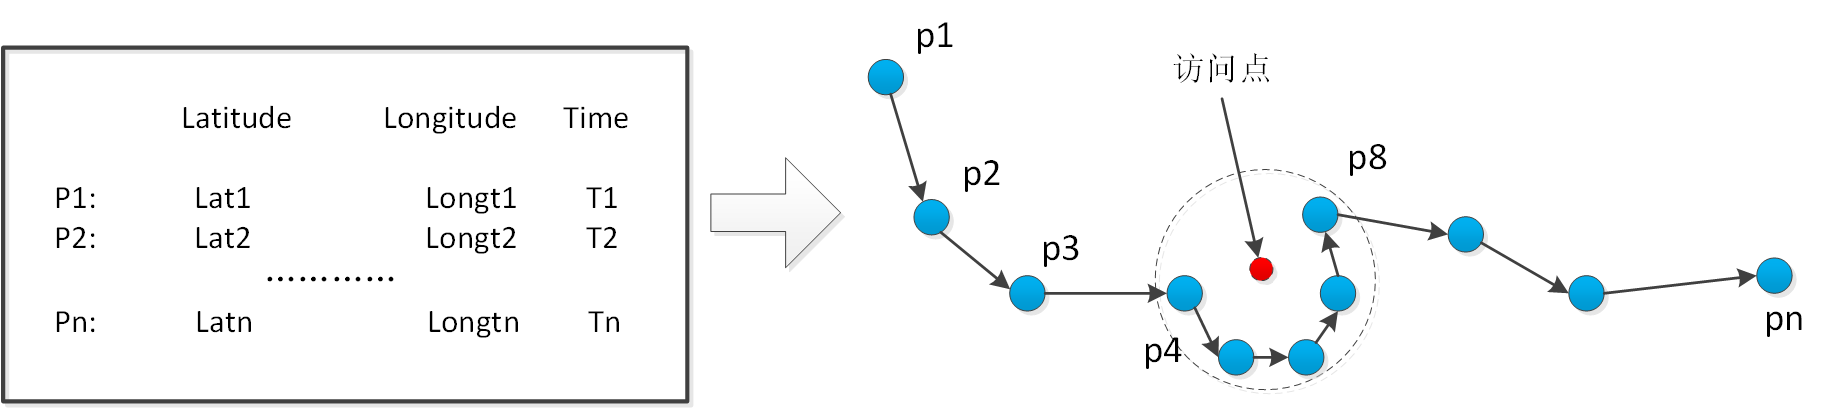
\includegraphics[width=0.8\textwidth]{figure2_1_gps}
\caption{用户GPS轨迹示例图}
\label{fig:2_1}
\end{figure}
\par 停留点的计算过程如\ref{alg2_1staypoint}所示。
\begin{algorithm}[htb]
\caption{停留点检测算法}
\label{alg2_1staypoint}
\begin{algorithmic}[1] %每行显示行号
				\REQUIRE 用户GPS轨迹 $Tra$,$\Delta T$,$\Delta_{distance}$
				\ENSURE 用户停留点序列$SP$
				%\Function {SPDec}{$Tra, \tau_{time},\tau_{distance}$}
				\STATE $i = 0$ , $PointNum= \left| \ Tra \right|$,$SP = Null$
				\WHILE {$i<PointNum$}
				\STATE $j = i+1$
				\WHILE {$j < PointNum$}
				\STATE $distance=Dis(Tra_{i},Tra_{j})$
				\IF {$distance > \Delta_{distance}$}
				\STATE $\Delta_{t}=Tra_{j}.T-Tra_{i}.T$
				\IF {$\Delta_{t} > \tau_{time}  $ }
				\STATE $p.Lat = avg(Tra_{k}.Lat)  $
				\STATE $p.Lng = avg(Tra_{k}.Lng)$
				\STATE $p.T = Tra_{i}.T(arv|lev)$%p.levT = Tra_{j}.T $
				\STATE $SP .add(p) ;j++; $
				\ENDIF				
				\ENDIF				
				\ENDWHILE
				\STATE $i=j ; break$
				\ENDWHILE
				\STATE \RETURN {$SP$}
				%\EndFunction				
\end{algorithmic}
\end{algorithm}
\subsection{聚类算法}
由于现实生活中人们可能会经常多次访问同一个空间地点,但是所计算得到的停留点却可能并不完全相同(坐标的变差,计算的误差等因素影响),因此采用传统直接比较停留点的方法不具备可行性。我们采取对停留点进行聚类的处理方法,这样地理位置非常相近的点就会被划分为同一个类别中。接下来介绍一些常用的聚类算法。
\par 聚类是属于无监督学习中的一种重要的方法,在其他的机器学习方法中如:回归分析、朴素贝叶斯网络等的数据都是带有类别标签$\gamma$,也就是说在训练集中的样例就已经给出了样例的类别,而聚类数据样本却没有给出样本类别$\gamma$聚类的目标是根据组内元素距离最小,组间距离最大将原始数据划分为若干组如图\ref{figure2_1cluster}所示。本节主要介绍几种常用的聚类分析方法:K-Means聚类算法、基于密度的DJ-Cluster 聚类算法以及近年发表的一种改进的基于密度的聚类算法。
\begin{figure}[htp]
\centering
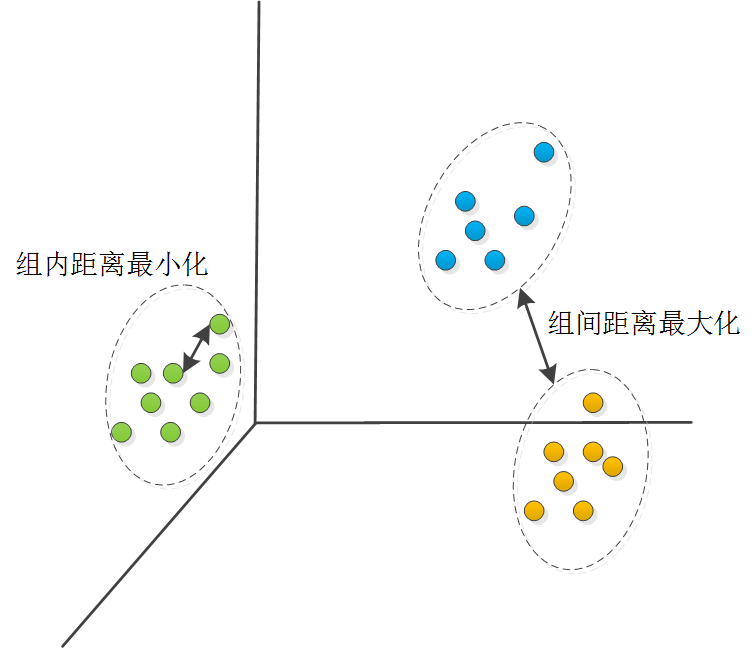
\includegraphics[width=0.8\textwidth]{figure2_1cluster}
\caption{聚类效果示意图}
\label{figure2_1cluster}
\end{figure}
\par  K-means聚类算法是比较经典的聚类方法之一,由J.MacQUEEN在1967提出\upcite{macqueen1967some}。该算法执行效率高,在大规模的数据处理聚类时被广泛使用,该算法输入$k$作为最终聚类的个数,将待分类的$n$个数据分成$k$个簇,使得簇内数据具有高的相似度而簇间的数据存在较低的相似度。K-means聚类算法的执行过程如下:首先根据输入的参数$k$随机从原始数据中选择$k$个对象,每个初始化的对象代表了一个簇的中心;其次,剩余的每个对象计算与簇中心的距离将它们赋予距离最近的簇;第一轮结束后将重新计算每个簇的中心,这个过程不断重复知道准则函数收敛或者簇没有新的变化为止,通常采用平方误差的度量准则如\ref{equ:chap2:k-means}:
\begin{equation}
\label{equ:chap2:k-means}
E=\sum_{i=1}^{k}\sum_{p\subset C}^{p}{\left | p-m_{i} \right |^{2}}
\end{equation}
\par K-means算法虽然简单,易于实现,但是在实际使用过程中需要用户指定$k$的取值,而$k$的取值是难以估计的,针对不同的数据事先并不可能确切的知道这些原始数据应该划分为多少个类别才正确;同时该聚类算法对异常数据非常敏感,一旦出现离群点将容易导致簇中心点出现漂移,对计算结果影响巨大。
%--------写到这里
\par 相比于前面描述的基于距离的聚类方法,研究者于2007年提出了一种基于密度的聚类算法DBSCAN\upcite{ester1996density}以及日后基于该算法改进的DJ-Cluster聚类算法\upcite{zhou2007discovering},DBSCAN算法的基本思想是扫描整个待分类的原始数据集,当扫描到数据对象P 时,计算P的$Eps$邻域内所密度可达的数据对象个数是否大于等于定义的$MinPts$,如果为真,则设立以P为核心的簇,然后尽可能的寻找与该簇密度相连的最大集合或者不断迭代查找该簇中每个数据对象的直接密度可达点,加入到该簇中。如图\ref{fig:figure2_2dbscan}中所示,设$MinPts=3$,从图中我们可以看出原始数据点M,P,O和点R的$Eps$邻域内说包含的点均大于等于$MinPts$因此都可以把它们标记为核心;M是P的直接密度可达,Q是M的直接密度可达。因此可以得知:Q是P的密度可达,但是P不是点Q的密度可达,点O,R和点S是密度相连的。通过实验证明,DBSCAN会受到$Eps$和$MinPts$取值的影响。
\begin{figure}[h]
\centering
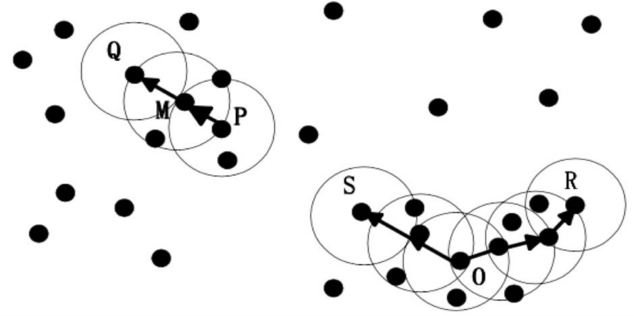
\includegraphics[width=0.8\textwidth]{figure2_2dbscan}
\caption{DBSCAN密度直达和密度可达示意图}
\label{fig:figure2_2dbscan}
\end{figure}
\par Rodriguez A等人2014年在Science上发表了一种新的基于密度的聚类算法\upcite{rodriguez2014clustering}。该算法相比较于之前的聚类算法,具有对参数不敏感便于输出正确的聚类结果的有点。该算法的主要改进想法是针对所有待聚类的组标点基于它们之间的距离,提出了两个新的标准属性:$\rho$和$\delta$,基于聚类中心点具有:中心点自身的密度大,即它的密度超过邻域集合点的密度同时距离其它密度大的中心点之间的距离也足够大这样的特征,其中局部密度$\rho$采用Cut-off kernel计算方式,公式如\ref{equ:chap2:Cut-off-kernel}所示,其中$p_{i}$表示S中与数据点$x_{i}$距离小于$d_{c}$的点的数量;$d_{c}$为截断距离需要用户事先设定并且保证$d_{c} >0$。
\begin{equation}
\label{equ:chap2:Cut-off-kernel}
\rho_{i}=\sum_{j \in I_{s}\setminus {i}}^{ }\chi (d_{ij}-d_{c})
\end{equation}
公式\ref{equ:chap2:Cut-off-kernel}中的$\chi(x)$的计算方式为:
\begin{equation}
\label{equ:chap2:chi-kernel}
\chi{x}=
\begin{cases}
1 & \mbox { $x<0$}\\
0 & \mbox { $x \geq  0$}
\end{cases}
\end{equation}
\par 算法中另一个指标距离$\delta$的定义为设$\left \{  q_{i} \right \}$表示$\left \{  p_{i} \right \}$的降序的下标序列,因此该序列满足:
\begin{equation}
\label{equ:chap2:se-delta}
\rho_{q_{1}} \geq \rho_{q_{2}} \cdots \geq \rho_{q_{N}}
\end{equation}
\par 则可根据公式\ref{equ:chap2:jisuan-delta} 计算出$\delta$:
\begin{equation}
\label{equ:chap2:jisuan-delta}
\chi{x}=
\begin{cases}
\underset{q_{j},j<i}{min} \left \{ d_{q_{i}q_{j}} \right \}  & \mbox { $i \geq 2$}\\
\underset{j\geq 2}{max} \left \{ \delta_{q_{j}} \right \} & \mbox { $i=1$}
\end{cases}
\end{equation}
该算法原理示意见图\ref{fig:2_3}和图\ref{fig:2_4},从图\ref{fig:2_4}可以看出,编号为1和编号为10的坐标点具有较大的$\rho$和$\delta$取值,因此在原始数据中我们将这两个点设置为簇的中心,而在图\ref{fig:2_3}中这两个坐标点恰好是分类簇的中心点;同时还出现了编号26-28三个“离群点”它们的特点是$\delta$值很大而$\rho$取值很小。
\begin{figure}[htp]
\centering
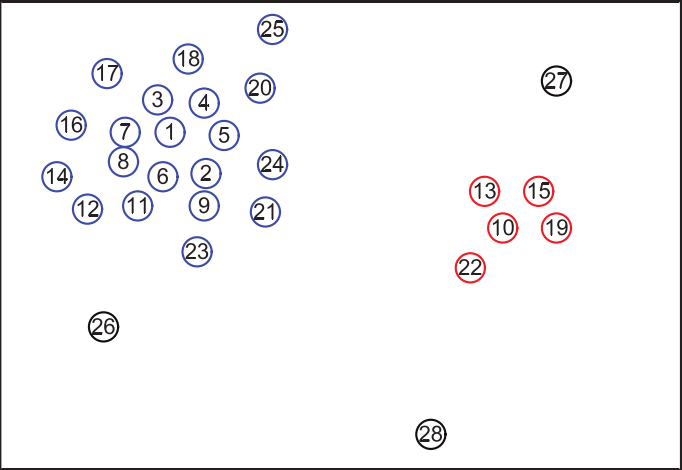
\includegraphics[width=4in]{figure2_3}
\caption{关于decision graph的示例\upcite{rodriguez2014clustering}}
\label{fig:2_3}
\end{figure}
\begin{figure}[htp]
\centering
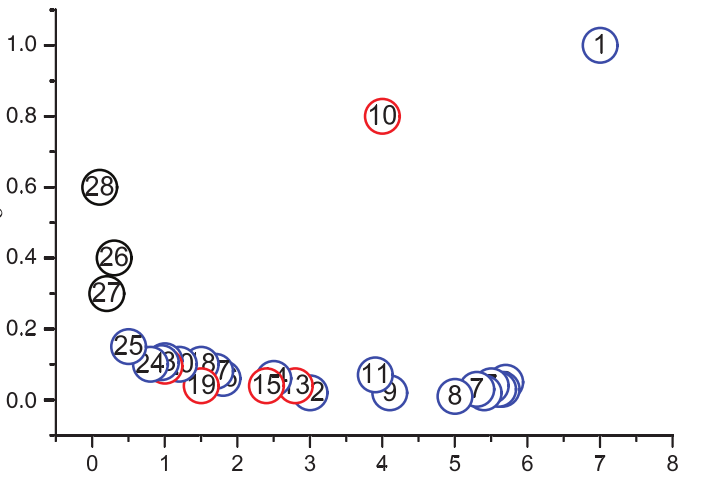
\includegraphics[width=4in]{figure2_4}
\caption{聚类中各点的$\rho$和$\delta$取值\upcite{rodriguez2014clustering}}
\label{fig:2_4}
\end{figure}
\par 总的来说,上述三种聚类算法通过精心调整参数都能取得非常好的聚类效果。不同的算法拥有不同的优缺点,在第四章我们将通过实验来展示各种算法在不同参数下的聚类结果。
\section{时间序列相似度度量方法}
\label{sec:section2-2}
我们阅读了大量社会心理学相关的论文书籍,从中证实得到在现实生活中关系亲密的两个用户会更加倾向于一起进行面对面的交流、共同进行社交活动等,因此通过对手机传感器数据的处理分析能够从中挖掘出人们现实生活中的关系强度。文献[37] 立足于空间距离,提出了在空间距离上非常接近的人们在现实生活中就越可能发生面对面的交互,该文献通过调研一个小区的住户发现人们在现实生活中越是接近,就越容易成为朋友。文献\cite{zajonc1968attitudinal}\cite{zillmann2000mood}进一步通过研究用户的轨迹数据发现由于在空间距离中接近的用户在现实生活中更可能产生交互行为,也就是说拥有相似日常生活轨迹的用户更可能产生交互活动。在现实生活中亦是如此,我们很容易和同自己经常出没同一个地点、行走在同一条轨迹上的人发展友谊关系。
\par 用户的轨迹序列由带有时间戳的位置数据构成,位置数据可能是GPS 也可能是基站号。因此我们可以将轨迹序列看作时间序列,从而使用一些时间序列相似度度量模型来度量轨迹的相似度,下面依次描述编辑距离和DTW这两种相似度度量方法以及序列熵值的计算方法。前面章节描述到用户的轨迹是由GPS位置点所构成的,包含了$(经度,纬度,时间戳)$等详细信息,因此我们将用户的轨迹看作一条由带有时间戳所构成的坐标点序列,采用序列相似度计算方式来处理轨迹之间的相似度。接下来详细描述两种常用的序列相似度计算方法。
\subsection{轨迹中心距离}
传统的计算序列相似度所采用的方法如:编辑距离、汉明距离和夹角余弦等有其优缺点,如果贸然用来计算用户轨迹序列的相似性可能不太符合实际问题的需求,在此基础上,Hechen Liu等学者提出了一种基于用户地理轨迹的相似度度量方法\upcite{liu2012similarity},根据用户的轨迹形状以及时间片内轨迹的中心点之间的距离来作为度量用户轨迹之间相似度的标准。如图\ref{fig:2_3_turn}中(a)图所示,现有两条用户轨迹$Tra_{1}=<a_{1},a_{2},a_{3},a_{4},a_{5}>$和
$Tra_{2}=<b_{1},b_{2},b_{3}>$从观测来看两条轨迹是非常相似的,但是从整条轨迹对比来看,就很难评判两条轨迹是否相似了,因为$Tra_{1}$中有一处急转弯点$a_{3}$,称为转折点。因此算法首先检测出轨迹中的转折点如图\ref{fig:2_3_turn}中(b)再针对每段轨迹中中心点(Center of mass)来计算轨迹之间的相似性。算法中的Center of mass是轨迹$Tra$的质量中心,计算公式如\ref{equ:chap2:Center_of_mass}所示,轨迹计算结果示意图如图\ref{fig:2_3_Center_of_mass}所示,最后再计算轨迹之间的距离,采用余弦相似度来衡量轨迹之间的相似性。
\begin{figure}[htp]
\centering
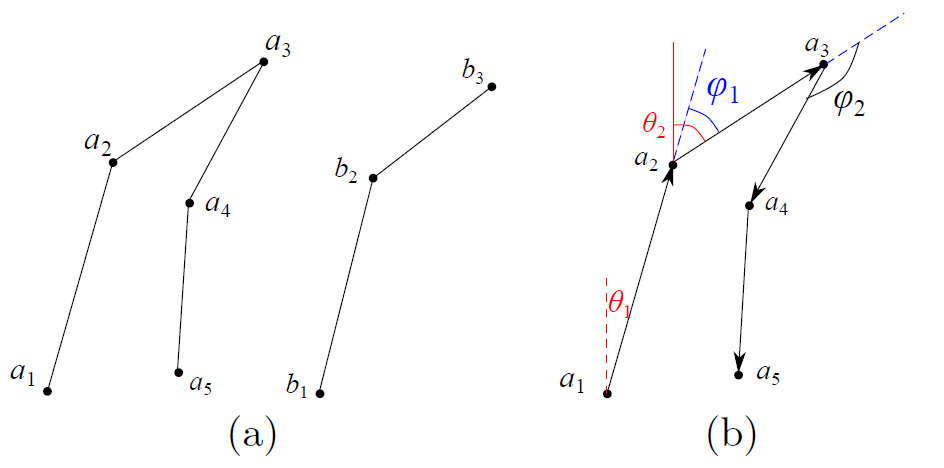
\includegraphics[width=0.8\textwidth]{figure2_1_turnTra}
\caption{轨迹相似计算示例\upcite{liu2012similarity}}
\label{fig:2_3_turn}
\end{figure}
\begin{equation}
\label{equ:chap2:Center_of_mass}
ctr(Tra)=(\bar{x},\bar{y})=(  \frac{\int x f(x)dx  }{\int f(x)dx},\frac{\int y f(y)dy  }{\int f(y)dy} )
\end{equation}
\begin{figure}[htp]
\centering
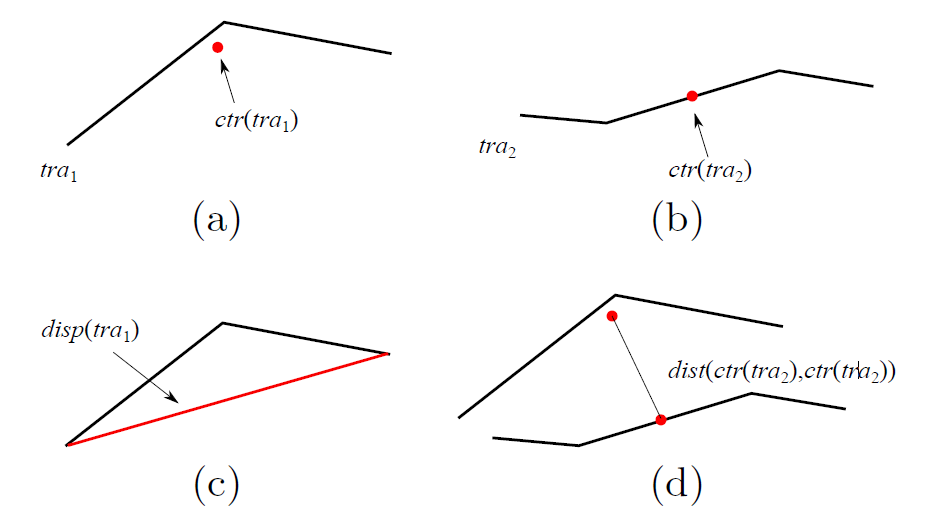
\includegraphics[width=0.8\textwidth]{figure2_1_Center_of_mass}
\caption{基于Center of mass轨迹计算示例\upcite{liu2012similarity}}
\label{fig:2_3_Center_of_mass}
\end{figure}
%-----------------写到这里
\par 采用该算法来计算用户轨迹之间的相似度同直接计算轨迹之间的欧氏距离相比较,能够将轨迹的形状考虑在内,这样能够结合避免直接计算轨迹之间的距离所因为离群点造成了计算结果的巨大偏差。
\subsection{Dynamic Time Warping}
DTW(Dynamic Time Warping)算法最初是由Itakura提出的的一种新型的计算距离的方法\upcite{itakura1987distance},在最初的一段时间是被应用于语音识别领域,在语音识别中即使是同一个词语,由不同的人说出口但是他们的语速、语气等不同造成了单词音频的差别。DTW正由于其计算距离的特殊处理使其能够胜任这一工作。DTW算法采用动态时间规整的思想,将需要比较的两个序列在横轴时间维度上进行压缩、拉伸等操作,使得两条序列具有相同的长度具有更有效的匹配度,同时也消除了传统基于欧式距离计算带来的弊端。
\par 设待计算距离的两个序列,序列$Q$和序列$C$ (两条序列的表示见公式\ref{equ:chap2:dtw_01}、\ref{equ:chap2:dtw_02})。如果两条序列的长度相同,则计算变得很简单。但是如果$m \neq n$,就需要拉伸变形两条序列,使得它们的长度能够尽量对齐同时保留原有序列的信息,算法首先构造一个$n \ast m$矩阵$d$,其中$d[i,j]$ 表示$q_{i}$ 和$c_{j}$之间的距离。采用动态规划的方法来找出序列$Q$和$C$之间的最佳匹配,其中转移方程为找出一条路径使得所有总和的距离$\gamma[i,j]$最小化,具体公式描述见公式\ref{equ:chap2:dtw_03}。
路径及矩阵可视化见图\ref{fig:2_5}。其中:A)为两个待计算比较的序列;B)为通过DTW动态规划求解后两条序列计算距离时所对应的点;C) 将原有序列所对应的位置进行拉伸展开后更加直观的DTW匹配计算结果示意图。
\begin{equation}
\label{equ:chap2:dtw_01}
Q=q_{1},q_{2},…,q_{i},…,q_{n}
\end{equation}
\begin{equation}
\label{equ:chap2:dtw_02}
C=c_{1},c_{2},…,c_{j},…,c_{m}
\end{equation}
\begin{equation}
\label{equ:chap2:dtw_03}
\gamma[i,j]=d[i,j]+min\{\gamma[i-1,j-1],\gamma[i-1,j],\gamma[i,j-1]\}
\end{equation}
\begin{figure}[htb]
  \centering%
  \subfloat[原始序列]{%
    \label{fig:dtw-1}
    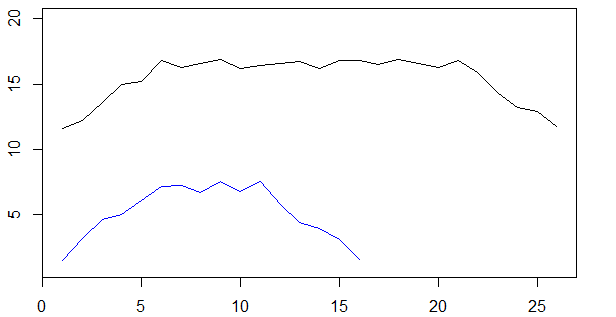
\includegraphics[width=0.4\textwidth]{dtw-1}}\hspace{2em}%
  \subfloat[DTW算法匹配模式结果]{%
    \label{dtw-2}
    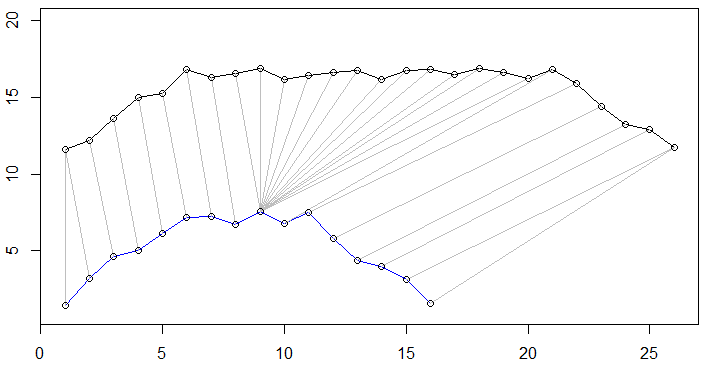
\includegraphics[width=0.4\textwidth]{dtw-2}}\hspace{2em}
    \subfloat[DTW算法拉伸序列计算距离]{%
    \label{dtw-2}
    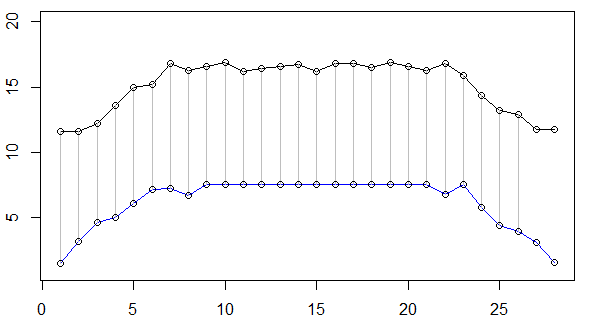
\includegraphics[width=0.4\textwidth]{dtw-3}}
  \caption{DTW算法匹配序列结果示意图}
  \label{fig:2_5}
\end{figure}
\par 通过对DTW算法的原理分析可以得知,序列$Q$和序列$C$的长度越长,则最终计算结果得到的距离就会越大。因此,后者研究中,采用了多种归一化的加权处理方法对结果进行加权处理\cite{ratanamahatana2004everything},获得最优的DTW计算结果。

\section{自然语言处理方法}
\label{sec:section2-3}
相对于用户的空间轨轨迹度量,用户在日常生活中的语义轨迹蕴含了更丰富的上下文信息同时人与人之间在语义轨迹层次上特别是好友之间可能表现出惊人的一致性,如经常去某些地方,在一天中总是先从某个地点出发,再经过某些地点,最后在某个咖啡店相遇等等。基于轨迹的用户模式的交互能够反映出用户在某个空间中的相遇;而基于用户语义轨迹的分析能够在一定程度上展现出用户在社会活动上的相似性,在绪论部分已经详细从社会心理学的研究中描述了人们在现实生活中相遇频率能够反映出用户之间的关系强度,文献\cite{singelis1994measurement}研究发现人们会更加喜欢那些在兴趣、价值观、人格上和自己相似的人。因此通过用户的语义轨迹来在更高的层次上对用户的行为进行相似度计算,进而推测出用户的关系强度。
\par 通过将用户的语义位置序集合同自然语言处理中的文档进行对比, 可以借鉴自然语言处理的算法来处理用户的语义轨迹序列。用户每天的活动轨迹通过语义标签标注后,得到的是一个现实生活中语义轨迹的序列集合,如将一个用户的活动轨迹表示为$<寝室,食堂,教室,图书馆,...,公园>$,通过结合自然语言文档文档相似性计算的思路,把用户每天所计算得到的语义轨迹作为一条原始自然语句,用户在$n$天内所采集的所有轨迹记录就生成了一篇文档,最后基于自然语言处理方法通过计算用户语义轨迹生成的文档之间的相似性来表示用户之间的关系强度。
\par 在以往的研究中,通常使用编辑距离来衡量语句的相似性。在用户轨迹相似分析上,文献\cite{farrahi2008did}借助了LDA主题模型来计算用户语义轨迹之间的相似性,后来的研究在其其基础上对计算方法进行了改进\upcite{yangruosong}。其算法改进在于基于LDA主题模型,将用户的所有语义轨迹看作一篇文档来训练出若干个主题。在计算用户轨迹相似性的时候,将用户用户估计输入到训练好的LDA模型中,然后采用余弦相似度分析比较二者输出的主题分布集合之间的相似度,作为这两个用户之间的关系强度。
\par word2vec是Google在2013年开源的一种词向量计算算法\upcite{mikolov2013efficient}, word2vec借鉴深度学习方法,将文本通过训练的得到文本的$K$维向量表示,通过词与词之间的距离来计算它们之间的相似度。
\subsection{LDA主题模型}
2003年文献\cite{blei2003latent}提出了LDA(Latent Dirichlet Allocation)模型对自然语言进行建模,可以用来识别文档语料中潜在的主题信息。整个计算模型采用了词袋的计算方法,计算出文档的向量表示,每一篇文档计算出一部分主题的概率分布,而每一个主题内又可以表示为很多词语的一个概率分布,LDA的训练过程为:遍历每一个文档,在主题分布袋中随机抽取一个主题;然后在被随机抽取到的主题中再随机抽取一个单词;最后重复上述步骤直到遍历完文档中的所有词语。整个生成的过程可以用图\ref{fig:2_6}表示:对于每一份文档与设定的$T$个主题之间的概率分布对应$\theta $,每个主题与词袋中的$V$个词语之间的概率分布$\phi$,其中$\theta $和$\phi$分别有一个参数$\alpha$和$\beta$的狄利克雷的先验分布,这样对于任意一份文档$d$中的每一词语,我们从与文档相对应的概率分布$\theta $中选取一个主题$z$,随即在根据与主题$z$对应的概率分布$\phi$中选取一个词语$w$,最后重复上述过程$N_{d}$次,就能够产生文档$d$,公式\ref{equ:chap2:lda_01}为LDA的核心公式。
\begin{figure}[htp]
\centering
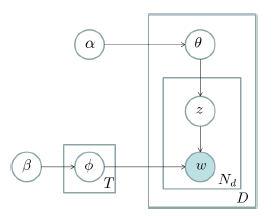
\includegraphics[width=0.6\textwidth]{figure2_6_lda}
\caption{LDA的图模型表示}
\label{fig:2_6}
\end{figure}
\begin{equation}
\label{equ:chap2:lda_01}
p(w|d)=p(w|t) \ast p(t|d)
\end{equation}
% 写到了这里------------------
\subsection{word2vec}
word2vec是Google在2013年开源的一种词向量计算算法\upcite{mikolov2013efficient}, word2vec借鉴深度学习方法,将文本通过训练的得到文本的$K$维向量表示,也就是说把特征转换到了$K$维空间进行表示,通过词与词之间的距离来计算它们之间的相似度。word2vec采用了三层的神经网络结构即为输入层-隐含层-输出层构成,其主要方法是借助哈夫曼编码针对相似词频的词语构建出相似的隐藏层激活函数,算法采用了层次化的Log-Bilinear模型,其中一种是基于CBOW(Continuous Bag-of-Words Model)的计算模型,在CBOW模型中,根据上下文信息可以预测下一个词语$w_{t}$,其公式如\ref{equ:chap2:word2vec_01}所示,CBOW的计算模型如图\ref{fig:2_7_cdow}所示。
\begin{equation}
\label{equ:chap2:word2vec_01}
p(w_{t}|context)=p(w_{t}|w_{t-k},w_{t-k+1},\cdots ,w_{t-1},w_{t+1},\cdots w_{t+k})
\end{equation}
\par 现在的CBOW计算采用层次的Softmax算法,每个单词$w_{i}$都可以有一条从根节点出发被唯一访问到的路径,这条路径就形成了词语的编码。
\begin{figure}[htp]
\centering
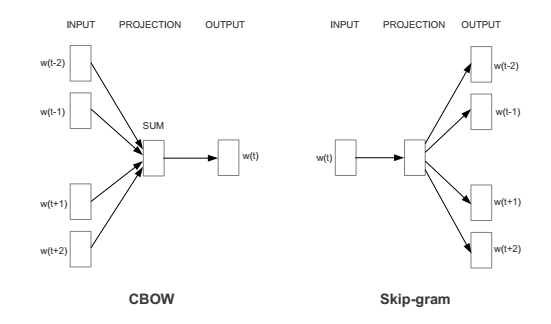
\includegraphics[width=0.8\textwidth]{figure2_7_cdow}
\caption{word2vec神经网络结构图\upcite{mikolov2013efficient}}
\label{fig:2_7_cdow}
\end{figure}
\begin{figure}[htp]
\centering
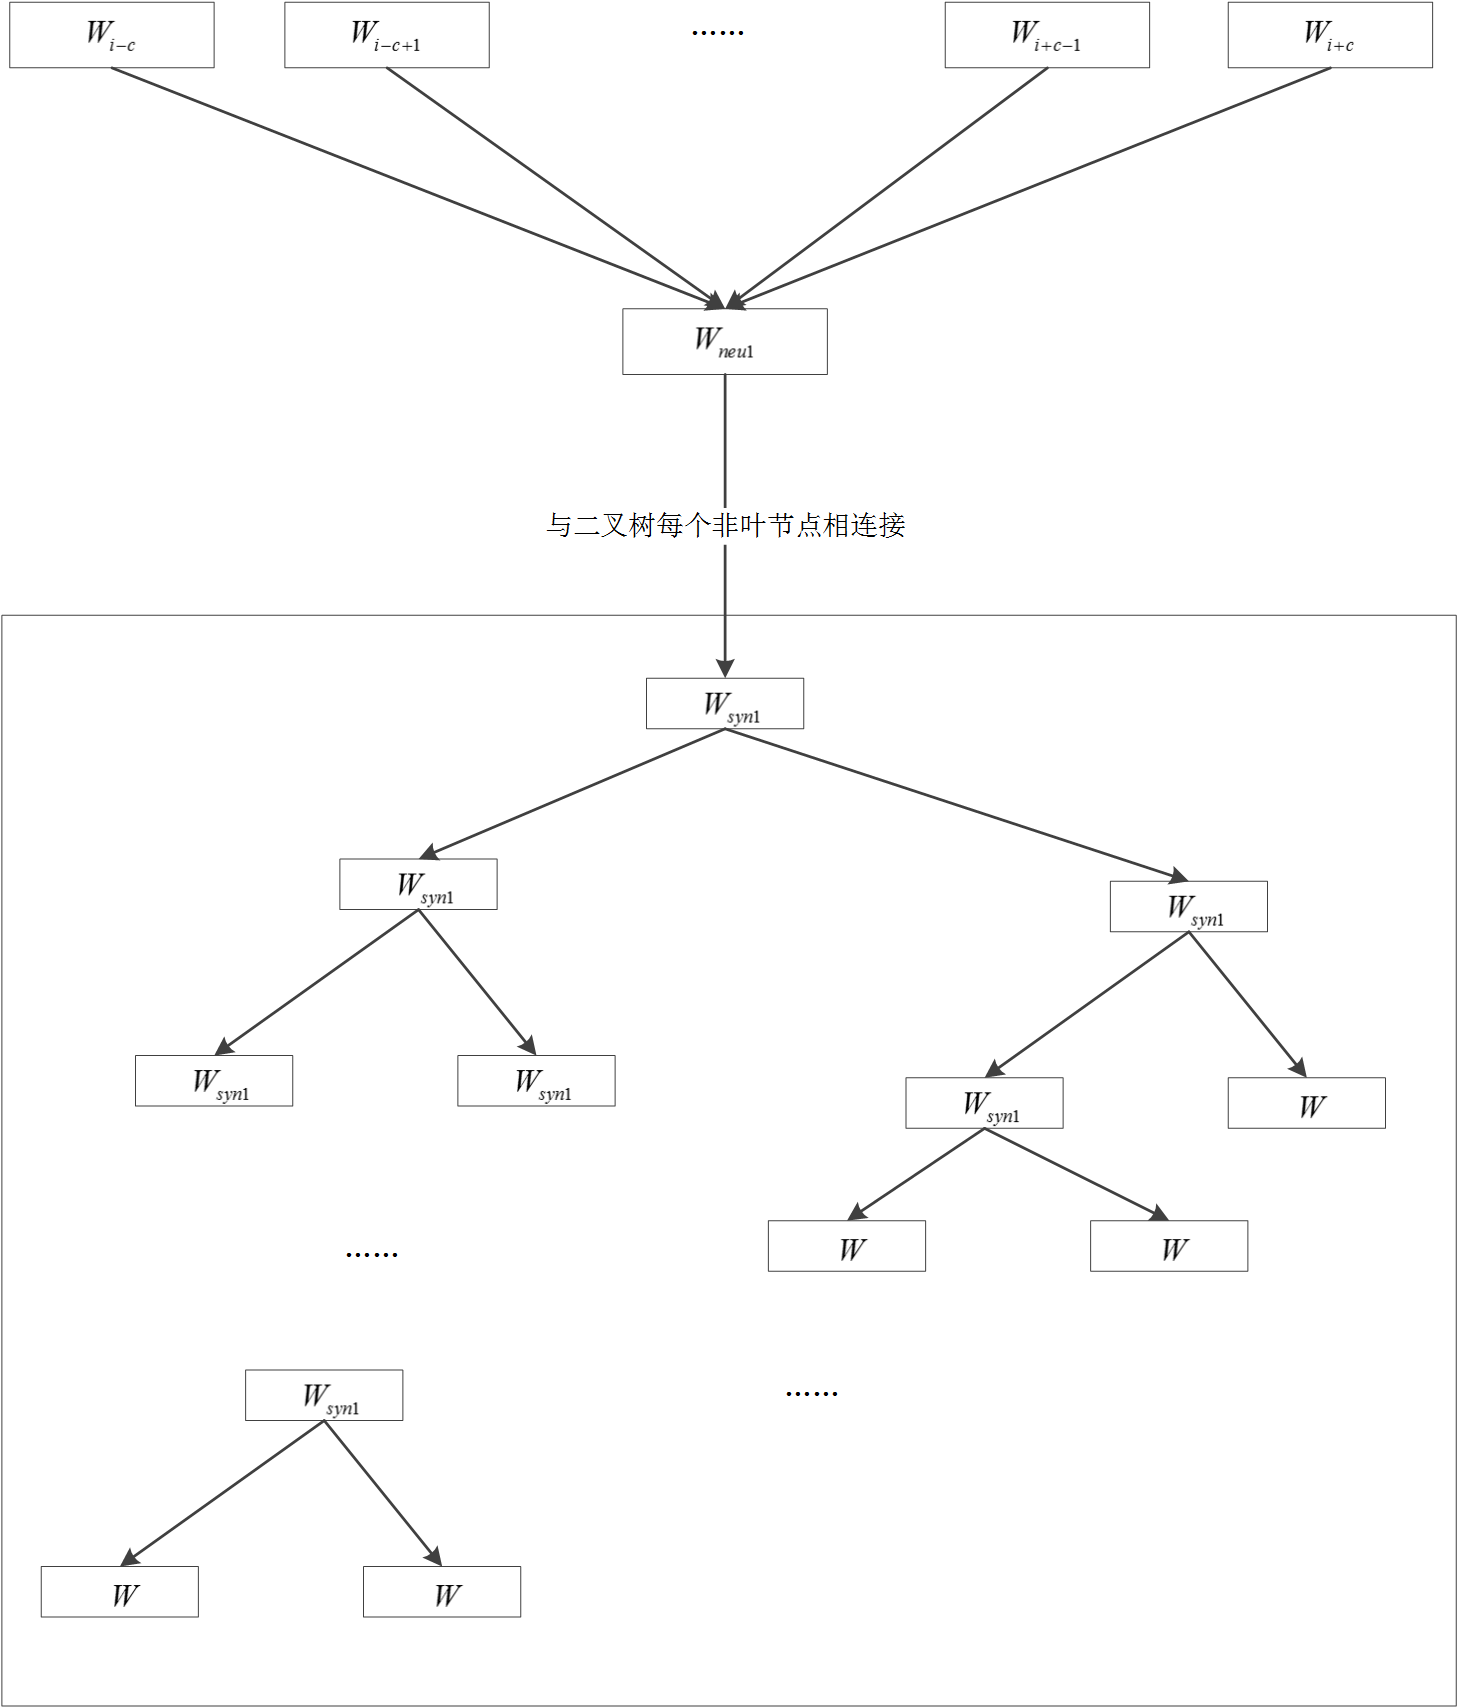
\includegraphics[width=0.7\textwidth]{figure2_7_w2cmodel}
\caption{word2vec神经网络结构图}
\label{fig:2_7}
\end{figure}
\par 在图\ref{fig:2_7}中,第一层也称之为输入层, 它的输入是词向量;中间的层次为隐含层,得到的的输入是输入层若干个词向量的向量累加结果;第三层则是由二叉树所构成的霍夫曼树所组成的输出层,其中每个非叶节点是一个计算后的向量但是不同于输入层的词向量,这里计算后的向量不代表某个词语,而是表示一个类别的词语,同时这棵霍夫曼树的所有叶子节点包含了输入词袋中的所有词。
\par 对于词袋$BG$中的单词$w$,在图\ref{fig:2_7}中一定能够找到有且仅有一条从Root节点到叶子节点$w$的路径。路径中的每一次分支都是一个概率问题,因此得到\ref{equ:chap2:word2vec_01}中的数学表达式,将其中的$w_{i}$用词向量替换,得到该三层神经网络的目标公式如\ref{equ:chap2:w2v_03}, $Num^{w}$表示从Root节点到词向量节点$w$路径中包含的节点个数,$w_{j}$表示该路径上的第$j$个词,$v_{w}$表示词$w$对应的词向量,$\sigma$表示SIGMOID函数,通过求解目标函数的最大值,就可以得到每个词所对应的向量。
\begin{equation}
\label{equ:chap2:w2v_03}
L=\sum_{w\in C}\sum_{j=2}^{Num^{w}}\{(1-w_{j})log[\sigma(v_{w}^{T}\theta_{j-1}^{w})]+w_{j}log[1-\sigma(v_{w}^{T}\theta_{j-1}^{w})]\}
\end{equation}
\subsection{快速Hash算法}
基于word2vec的计算方法针对文档的分词结果,再根据神经网络模型计算得到每个词的向量表示,但是这样无疑增加了整个计算过程的时间复杂度,本文研究目的是能够为众多用户提供一种计算关系强度的框架,因此如果采用传统的Hash算法进行处理,则能够减少程序的运行时间,来自于GoogleMoses Charikar针对海量文档快速计算相似计算提出了一种局部敏感hash算法\upcite{manku2007detecting},其核心内容恰巧和word2vec相反:希望将数据进行降维处理,将原始的高维词向量通过一系列运算映射到低维的词向量,最后来计算相似性。
\par 以上介绍了几种方法在自然语言处理中都得到了广泛的应用,因此综合考虑使用最后一种方法来作为计算方法, 在后面还会详细讲解如何使用hash来度量用户之间的关系强度,以及在不同处理方法之间进行横向和纵向的比较。
\section{WiFi和蓝牙数据的度量方法}
WiFi和蓝牙作为一种主动对外界感知和探索所得到的感知信息,已经证实能够被用来分析用户之间的社交关系。文献\cite{hsu2007mining}通过收集到用户的WiFi数据,然后将用户的WiFi数据同现实语义位置进行关联,得到了WiFi的语义向量,这样就能够得到基于WiFi的用户活动轨迹序列,提出了一种新的模型AMVD(average minimum vector distance)来计算人与人之间的距离,其计算公式如\ref{equ:chap2:amvd}所示,其中$a_{i}$和$b_{j}$表示用户A和用户B之间的联合向量,$d(a_{i},b_{j})$表示计算二者向量之间的曼哈顿距离。
\begin{equation}
\label{equ:chap2:amvd}
AMVD(A,B)=\frac{1}{\left | A \right |}\sum_{\forall a_{i} \in A}^{ }  \mathop{\arg\min}_{\forall b_{j} \in B} d(a_{i},b_{j})
\end{equation}
\par 蓝牙数据和GPS轨迹数据都能够推测出用户之间的交互行为,蓝牙作为一种近距离的无线通讯手段,收到波长影响使得通讯距离只能是5-10米内,因此蓝牙感知数据能够进一步描述了用户之间在现实生活中的物理接触。前人的研究中,有根据蓝牙信息来简单计算出用户在现实空间中的面对面交互次数,从而推测出用户的社会关系情况\upcite{eagle2009inferring,zheng2013unsupervised}。在本文中,我们使用了新的数据结构来表示用户的WiFi、蓝牙感知数据,同时直接计算其感知上下文环境信息的相似度作为用户之间环境的相似度的参照。
\section{小结}
\label{sec:section2-4}
本章详细的从本课题研究的三个数据源出发对不同数据源的研究方法、现状进行了详细的分析和讨论。2.1节讨论了在用户原始GPS轨迹数据处理中要解决的三个主要问题:剔除异常点、停留点检测以及空间轨迹的聚类。2.2节则是介绍了计算用户轨迹序列相似度的常用方法,并以此结果作为用户的关系强度计算结果。2.3节从自然语言处理的角度介绍了常用的文档相似性检测计算方法,为计算用户语义轨迹的相似度提供了可行性算法。2.4节从WiFi和蓝牙数据处理计算角度出发,介绍了前人研究的计算方法理论,为本研究中所采取的基于上下文环境的计算方式作出铺垫。
\chapter{RSMHD用户关系强度计算框架模型}
\label{chap:chapter07}
上一章详细介绍了和本研究数据源相关的处理技术与方法,接下来这一章将主要介绍RSMHD的多维据源多维度的关系度量模型的整体框架结构。
\section{RSMHD模型框架描述}
\label{sec:section7-1}
本研究的主要内容是通过采集到的用户感知数据(GPS轨迹信息 、WiFi数据、蓝牙数据)来开展用户之间的关系强度度量工作。因此本文希望能够提供一种基于此类非社交的感知数据建立的通用的用户关系强度计算框架。非社交数据主要是指不是来自于用户直接社交活动中所收集到的数据,在本研究中主要包含了用户轨迹数据、用户WiFi感知数据和用户蓝牙感知数据。因此本课题基于以上三种不同的感知数据源提出了能够统一处理多种数据源的计算框架,其整体概要结构图如图\ref{fig:7_1}所示,图中描述整体架构由以下几部分组成:上下文感知收集模块、基于用户日常轨迹的关系强度计算模块、基于用户WiFi感知数据的关系强度计算模块和基于用户蓝牙的关系强度计算模块。用户的日常语义轨迹是有连续的GPS位置点所组成的轨迹的集合,在用户的轨迹信息的采集过程中,因受到地形、气候、GPS 传感器的干扰误差的影响,会出现GPS漂移现象,GPS的位置漂移使得用户的轨迹数据中存在大量的噪音数据,影响后续对数据的处理和分析。因此对采集到的用户轨迹数据采取滤波处理,消除轨迹中所蕴含的噪音数据。GPS 位置的采集还受到地形环境的影响,在室内无法获取GPS 位置信息的时候会导致用户轨迹的缺失,造成计算结果产生巨大偏差。第四章部分将重点针对上述问题展开GPS轨迹的处理研究工作,以获得好的信息效果。对于剩余的WiFi和蓝牙感知数据来讲,主要的工作是针对二者数据源的特点以及后续的算法输入对原始数据进行提取和结构化建模表示存储。第四章的其余部分将会针对WiFi和蓝牙感知数据的预处理和结构化表示进行详细的描述。
\begin{figure}[htp]
\centering
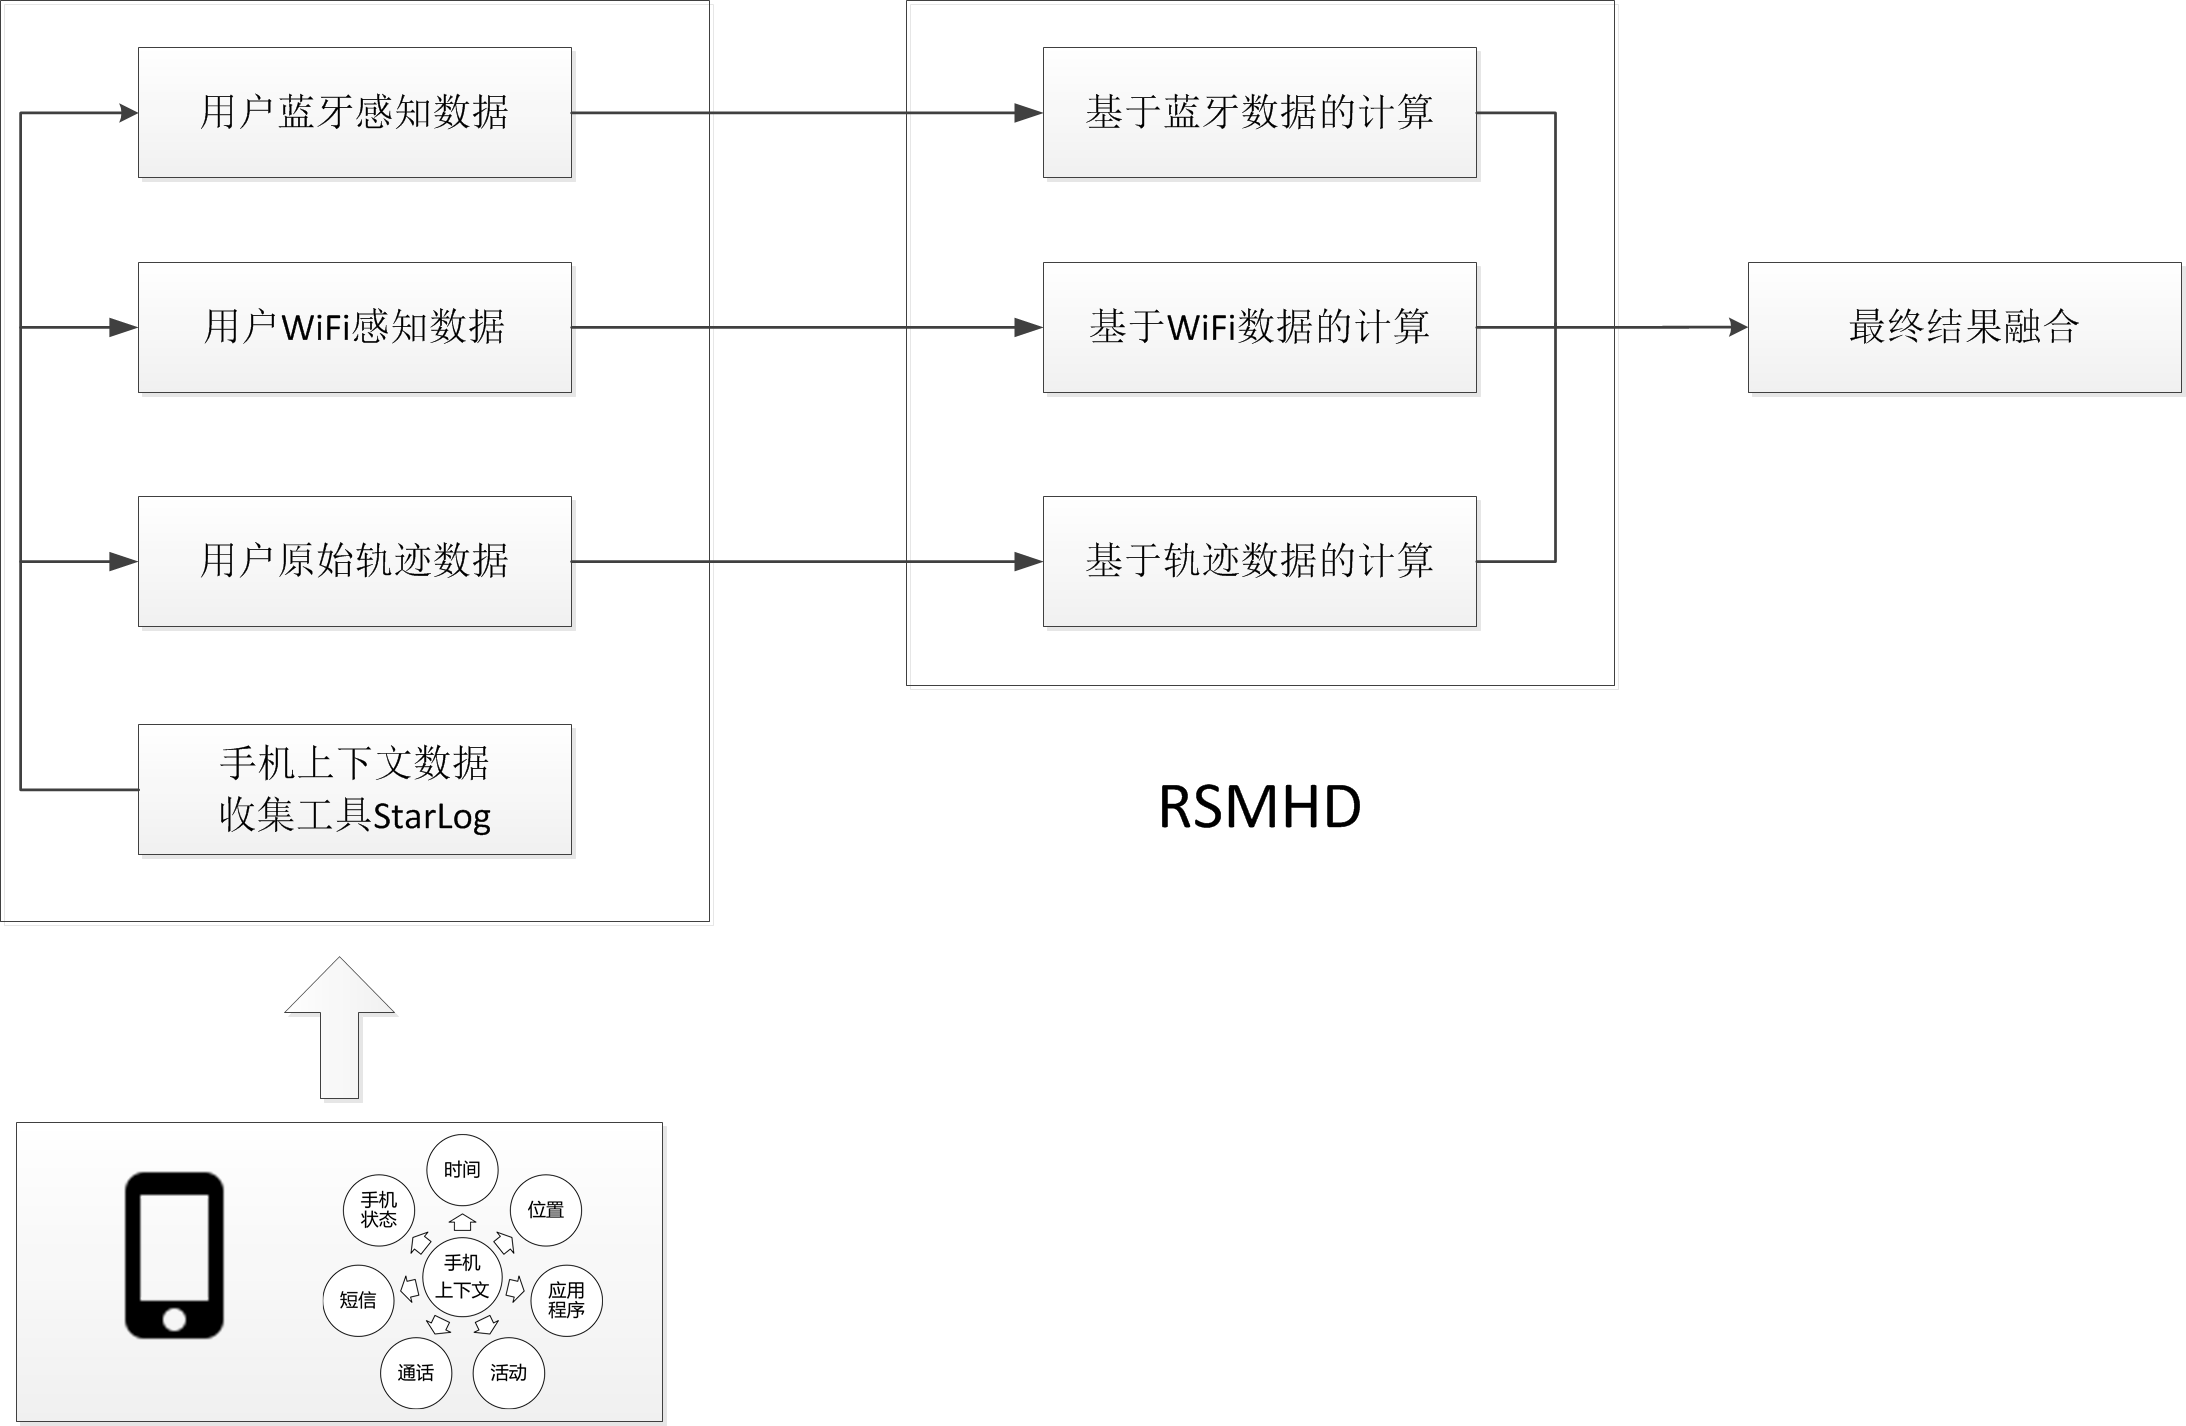
\includegraphics[width=0.8\textwidth]{figure7_1_RSMHD}
\caption{RSMHD用户关系强度计算模型框架图}
\label{fig:7_1}
\end{figure}
\subsection{基于轨迹数据的关系强度计算模块概述}
在本研究中所提出的RSMHD计算框架模型中,第二层需要基于用户的日常语义轨迹分别通过计算地理轨迹相似性、用户的语义轨迹相似性以及日常轨迹运动模式三个层次关系强度融合为轨迹强度结算结果,其详细框架图如图\ref{fig:7_1_tra}所示。在这个模块中,通过计算用户日常地理轨迹的相似性推测出用户之间的关系强度;针对用户活动产生的日常语义轨迹,RSMHD 模型采利用自然语言处理的思想,通过快速编码变换计算出用户基于语义轨迹的关系强度;第三层中,RSMHD 进一步挖掘出用户轨迹中更高一层的上下文信息(High Context)得出用户日常轨迹模式如:用户A 经常喜欢到校外某地用餐、用户B 经常下午在操场跑步等这些代表用户日常轨迹活动模式的信息,计算用户之间基于运动模式的关系强度。
\begin{figure}[htp]
\centering
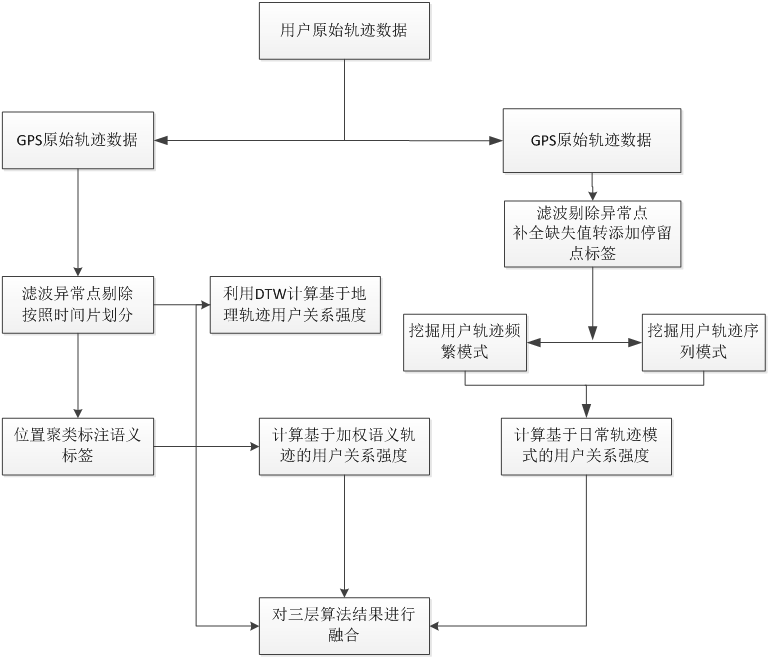
\includegraphics[width=0.8\textwidth]{figure7_1_tra}
\caption{RSMHD中基于用户轨迹计算模块详细框架图}
\label{fig:7_1_tra}
\end{figure}
\subsection{基于WiFi和蓝牙数据的关系强度计算模块概述}
在RSMHD计算框架模型中我们针对WiFi和蓝牙原始数据的特点以及现实生活中WiFi和蓝牙上下文环境的特征,采用了区别于原有基于WiFi和蓝牙计算社交关系的方法,整体的详细计算框架如图\ref{fig:7_1_wifi}所示。在WiFi和蓝牙数据处理计算框架中,分别针对底层手机的上下文感知信息进行数据信息的提取的规整,从复杂冗余的信息中萃取出关键的富有价值的信息;然后结合WiFi和蓝牙各自的上下文环境特征信息,将整理后的数据用图的数据结构进行结构化表示,使得抽象表示后的数据结构更加符合现实中的含义;最后基于结构化后的感知数据进行关系强度计算,将结果输出到下一层。
\begin{figure}[htp]
\centering
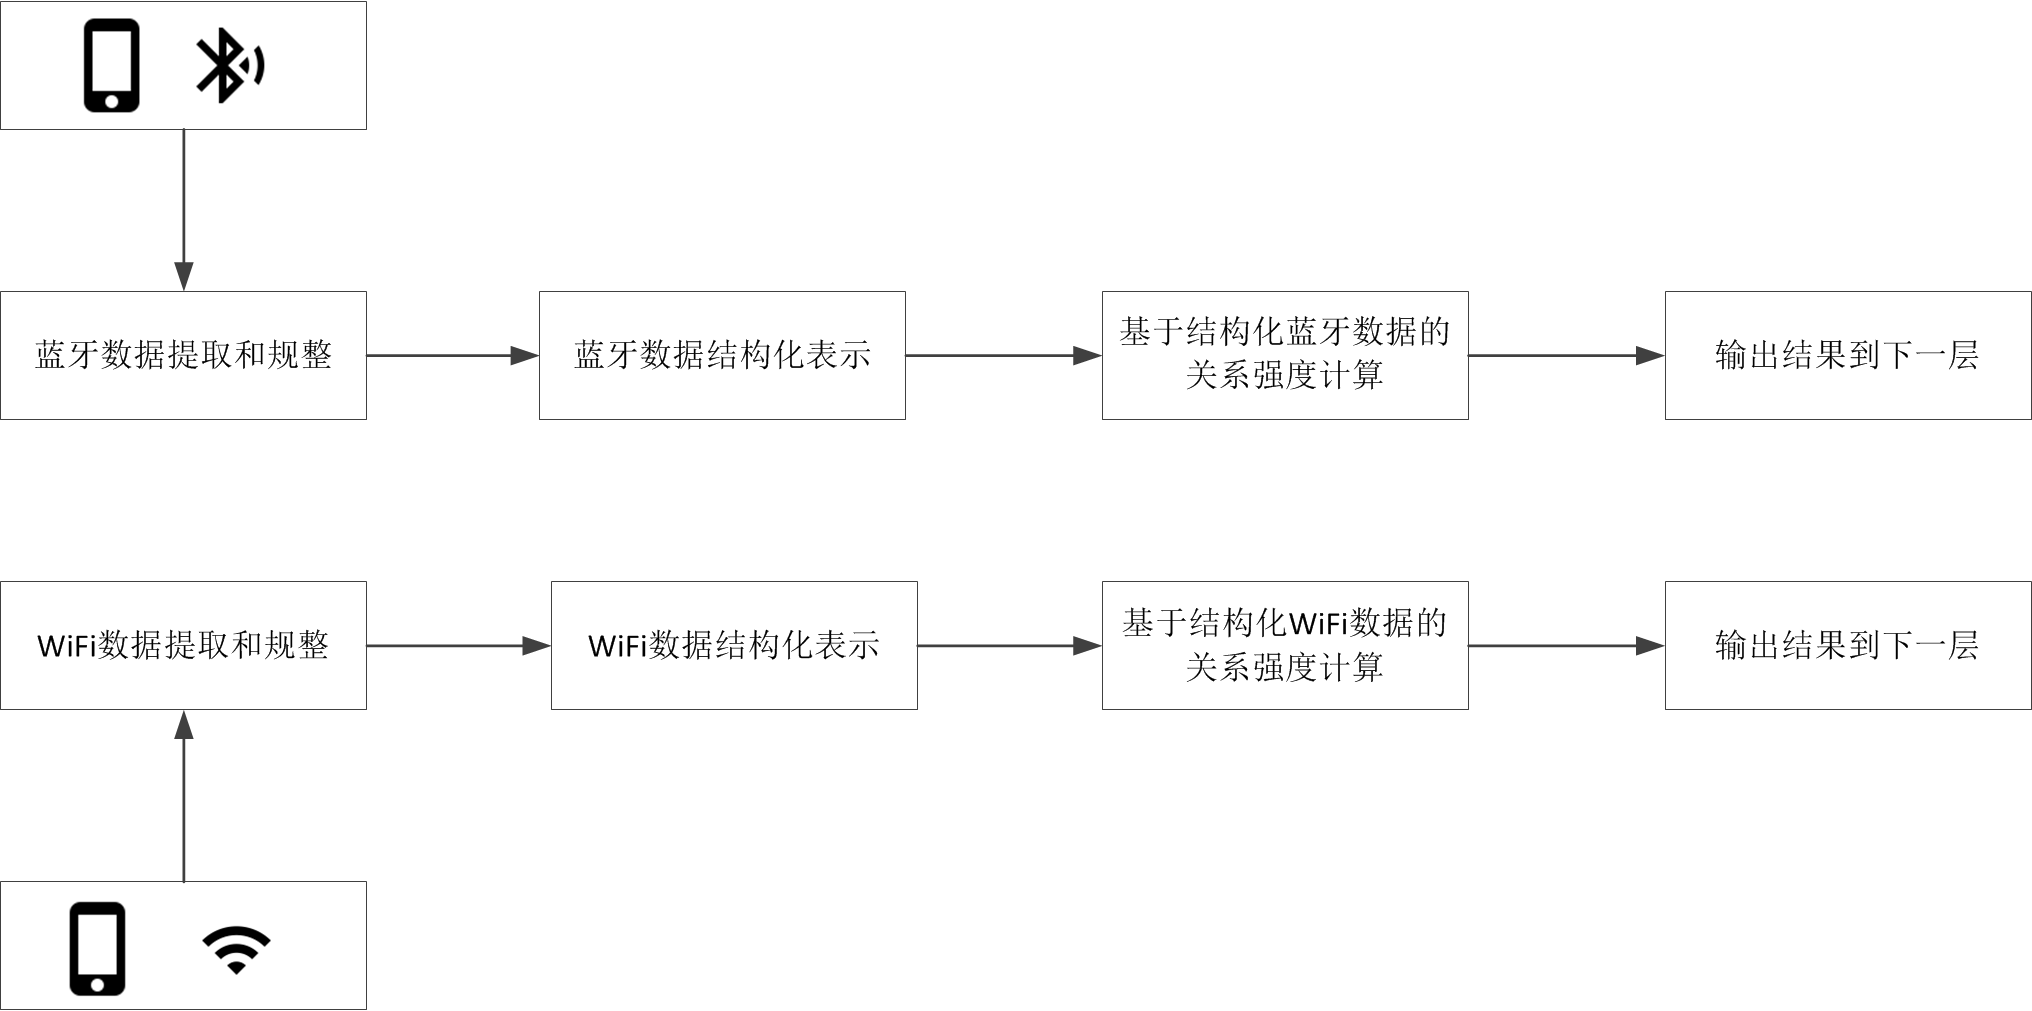
\includegraphics[width=0.8\textwidth]{figure_3_RSMHDwifibluee}
\caption{RSMHD中基于WiFi和蓝牙计算模块详细框架图}
\label{fig:7_1_wifi}
\end{figure}
\section{RSMHD模型计算流程概述}
\label{sec:section7-2}
整个信息采集是采用我们自己编写的用户手机上下文信息收集工具StarLog来记录保存用户手机的上下文感知数据如:GPS位置信息、WiFi感知信息、蓝牙感知信息、脱敏的通话记录、短信记录、APP使用记录等。
\par 针对用户的GPS位置数据我们首先对轨迹数据进行预处理,即采用滤波算法检测出用户日常轨迹中的漂移点减少轨迹中的噪音;然后根据停留点检测算法识别出用户轨迹中的停留点,针对缺失的轨迹点进行预测补全;第一层次中针对用户日常空间轨迹相似性计算时,可用将每天的轨迹数据划分为若干时间片的数据,然后采用DTW加权算法对时间片内的空间轨迹相似度进行计算并按照一天的轨迹进行处理。对于基于用户语义轨迹推倒关系强度这层我们首先将得到的停留点进行聚类分析,得到聚类后的停留点集合因此对于每一个簇都是同一个语义位置,然后将聚类GPS转换为现实社会中的语义标签,在计算用户语义轨迹的相似性时,采用快速hash算法将用户分片后的语义轨迹序列作为输入,得到用户之间每天的语义轨迹相似度,以及最终的语义轨迹相似度并将结果作为用户自己的关系强度。在上一层的基础上,我们针对得到的用户语义估计进行挖掘,寻找出用户的日常运动模式,然后计算用户运动模式之间的相似度并作为关系强度之一进行输出,综合三层的计算结果得到用户基于轨迹数据计算得到的关系强度。
\par 其次针对用户的WiFi和蓝牙数据,首先从原始数据中提取出重要的信息,并将WiFi和蓝牙数据进行结构化存储处理,采用图的存储结构,将WiFi和蓝牙数据还原为现实生活中的存在环境,然后针对用户切片时间内每刻的感知环境进行相似度计算,并将一天中的计算结果进行汇总进一步得到所有时间段内的用户相似度,最后将结果作为基于两种数据源推测出的用户关系强度。
\par 最后,在基于前面三种数据源的用户关系强度计算结果的基础上,采用集成学习的思想对计算结果进行融合处理,得到最终的用户关系强度计算结果。

\chapter{RSMHD框架的相关技术研究}
\label{chap:chapter03}
上一章节主要是对本课题研究的RSMHD框架进行了详细的描述,本章接下来将针对每一个模块中的具体面对的问题以及采取的方法进行详细描述,包括噪音点的剔除、如何语义轨迹、如何计算轨迹相似性以及如何对WiFi和蓝牙数据进行结构化处理等。
\section{GPS轨迹处理计算技术}
\label{sec:section3-1}
用户的日常GPS轨迹数据包含了用户的生活工作以及娱乐等丰富的上下文信息,如图\ref{fig:tramodel}所示,我们基于用户的日常轨迹分别从地理位置相似性、语义轨迹相似性以及轨迹模式相似性出发度量人与人之间的关系强度。模块的输入是由StarLog收集的GPS感知数据,通过对初始数据的解析提取得到原始的GPS位置点构成的用户轨迹序列。预处理阶段主要是通过滤波算法对原始轨迹序列进行异常点检测,并通过轨迹预测补全缺失的部分GPS轨迹序列;第二层中将第一层得到的停留点赋予语义得到用户的语义轨迹序列,采用自然语义处理思想计算基于语义轨迹的相似性;再往上一层,从用户的历史轨迹数据中挖掘出的频繁模式和序列模式能够反映出用户的日常轨迹运动习惯和行为规律,运动模式在现实生活中表现为用户经常行走的路径序列,是用户轨迹数据规律的抽象表示,最后计算用户之间的关系强度。
\begin{figure}[htp]
\centering
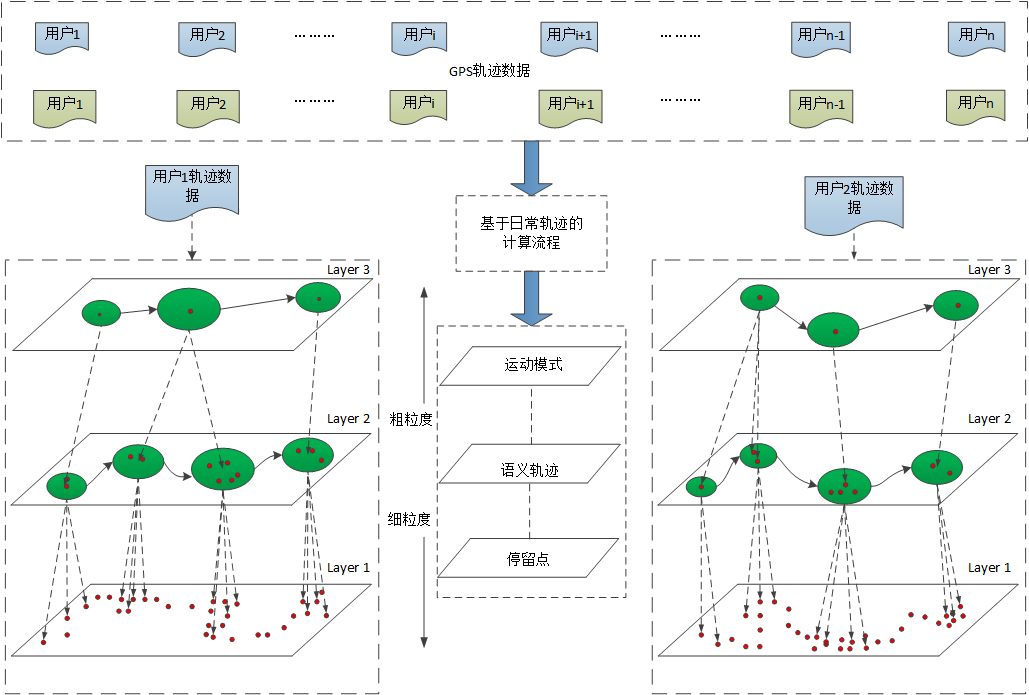
\includegraphics[width=0.8\textwidth]{figure4_2}
\caption{基于多层次多粒度轨迹的用户关系强度计算}
\label{fig:tramodel}
\end{figure}
\section{GPS轨迹预处理与语义化}
\label{sec:section3-2}
本节主要讲述如何对GPS轨迹数据进行清洗规整,以及得到用户的语义轨迹进行结构化存储。
\subsection{剔除轨迹中的异常点}
前文已经提到,由于在获取GPS位置信息的时候会受到位置漂移的影响,导致在获取用户实际位置的时候可能产生采样的误差甚至跳跃,为了使得最终计算得到的关系强度结果更为准确我们需要对GPS轨迹数据进行滤波分析。在第二章中描述了常用的三种滤波方法,在本章中将会针对三种滤波算法进行最后结果展示并根据结果分析最终采用此滤波算法的原因。
\par 首先接下来使用我们自己开发的用户感知数据收集软件StarLog,来分析观察各种滤波算法对用户轨迹中异常点检测剔除的效果,如图如图\ref{fig:3_2_1}、\ref{fig:3_2_2}所示。
\begin{figure}[htb]
  \centering%
  \subfloat[原始轨迹数据]{%
    \label{fig:3_2_1_1}
    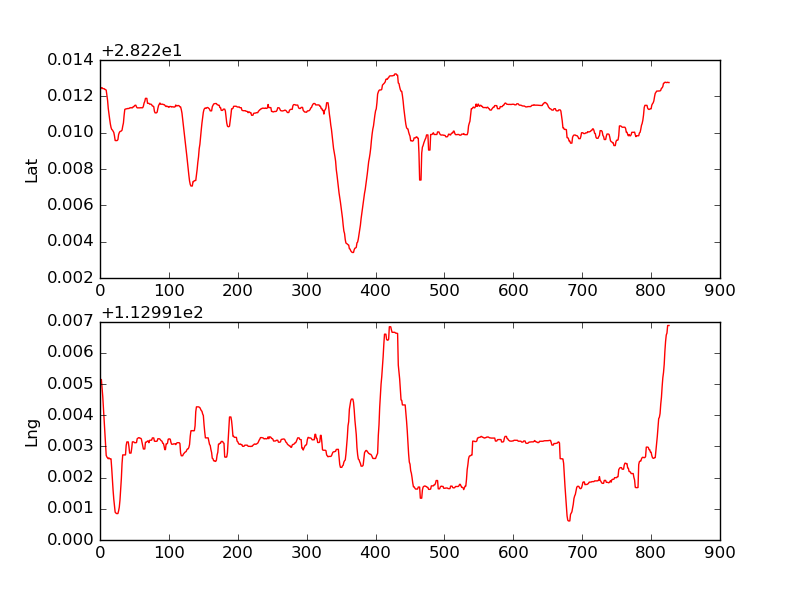
\includegraphics[height=4cm]{figure_4_mid_location1}}\hspace{4em}%
  \subfloat[中值滤波后的轨迹数据]{%
    \label{fig:3_2_2_1}
    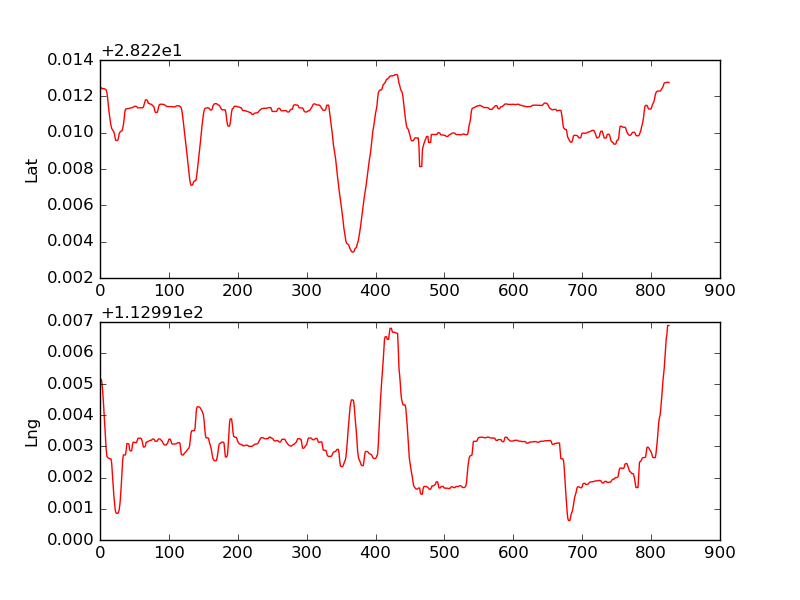
\includegraphics[height=4cm]{figure_4_mid_location1_ed}}
  \caption{轨迹中值滤波实验结果1}
  \label{fig:3_2_1}
\end{figure}
\begin{figure}[htb]
  \centering%
  \subfloat[原始轨迹数据]{%
    \label{fig:3_2_2_1}
    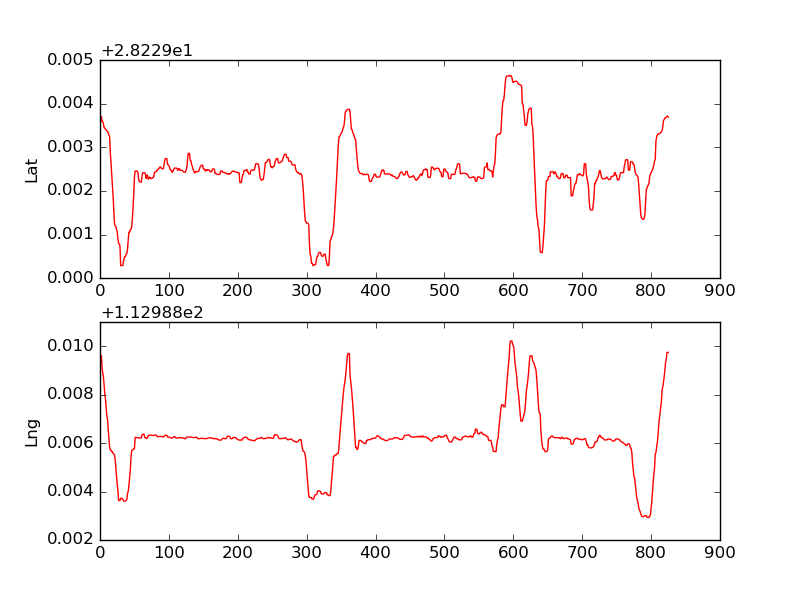
\includegraphics[height=4cm]{figure_4_mid_location2}}\hspace{4em}%
  \subfloat[中值滤波后的轨迹数据]{%
    \label{fig:3_2_2_2}
    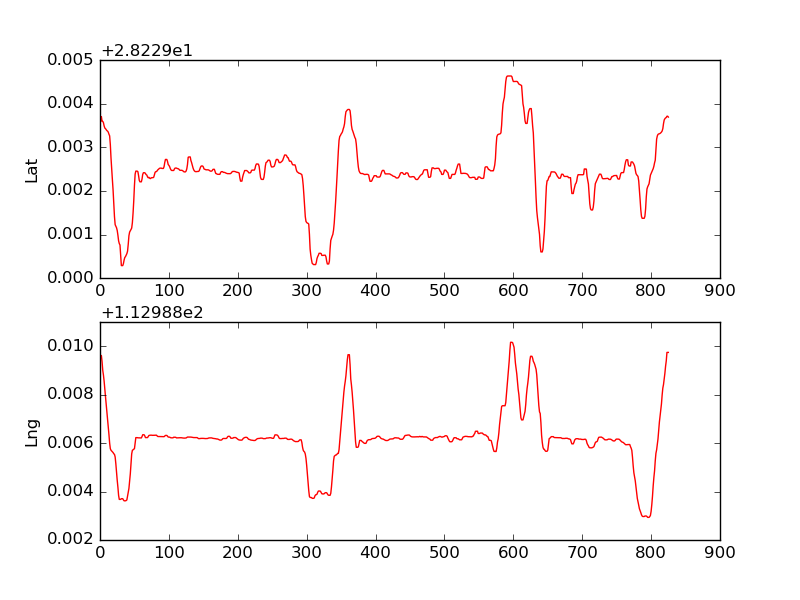
\includegraphics[height=4cm]{figure_4_mid_location2_ed}}
  \caption{轨迹中值滤波实验结果2}
  \label{fig:3_2_2}
\end{figure}
\par 从实验结果中我们可以观察到虽然中值滤波能够过滤掉其中少部分的位置漂移点,但是针对于一些明显的轨漂移点却没有能够很有效的识别过滤。
\par 接下来我们再使用均值滤波算法对用户轨迹进行分析,观察均值滤波算法对用户轨迹中异常点的检测情况,部分实验结果见图图\ref{fig:3_3_1}、\ref{fig:3_3_2}。
\begin{figure}[htb]
  \centering%
  \subfloat[原始轨迹数据]{%
    \label{fig:3_2_1_1}
    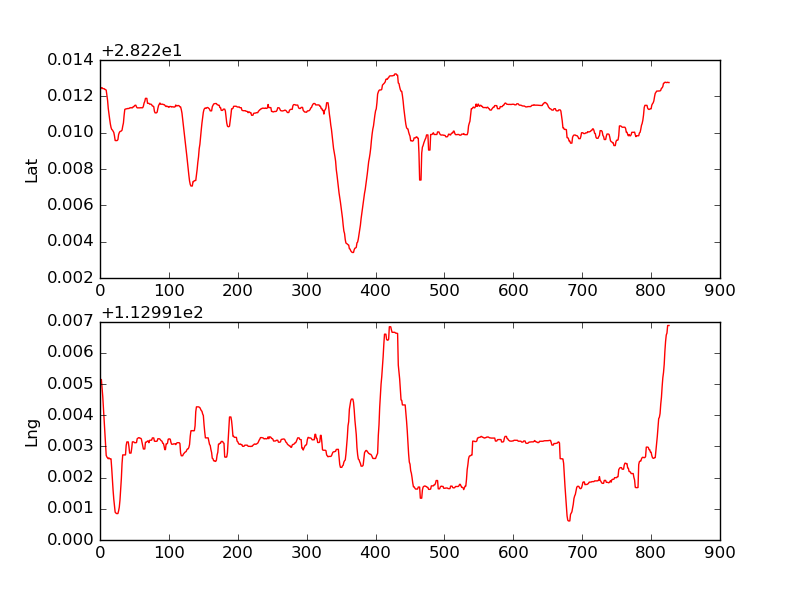
\includegraphics[height=4cm]{figure_4_mid_location1}}\hspace{4em}%
  \subfloat[均值滤波后的轨迹数据]{%
    \label{fig:3_2_2_1}
    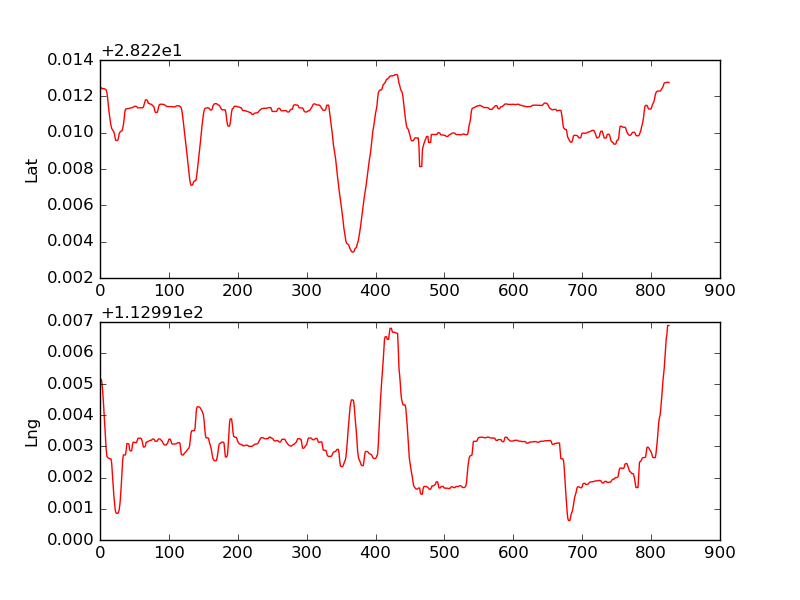
\includegraphics[height=4cm]{figure_4_mid_location1_avg}}
  \caption{轨迹均值滤波实验结果1}
  \label{fig:3_3_1}
\end{figure}
\begin{figure}[htb]
  \centering%
  \subfloat[原始轨迹数据]{%
    \label{fig:3_2_2_1}
    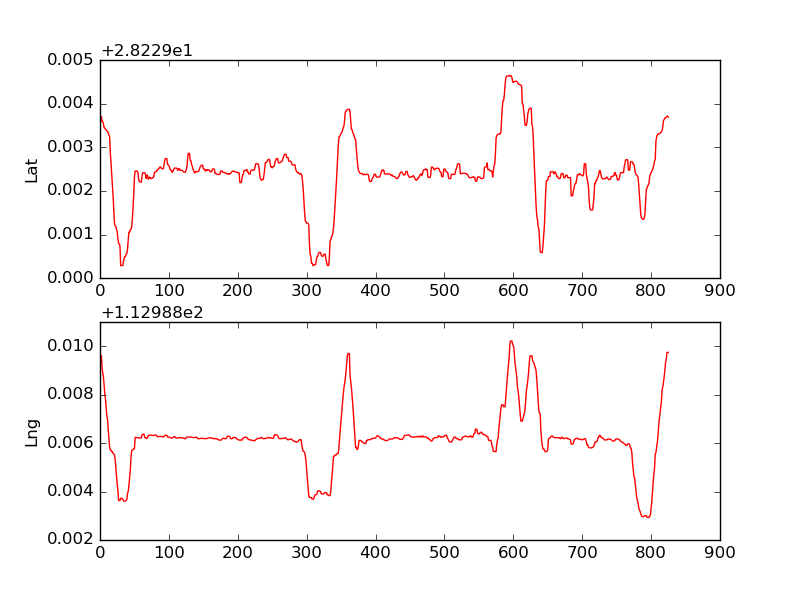
\includegraphics[height=4cm]{figure_4_mid_location2}}\hspace{4em}%
  \subfloat[均值滤波后的轨迹数据]{%
    \label{fig:3_2_2_2}
    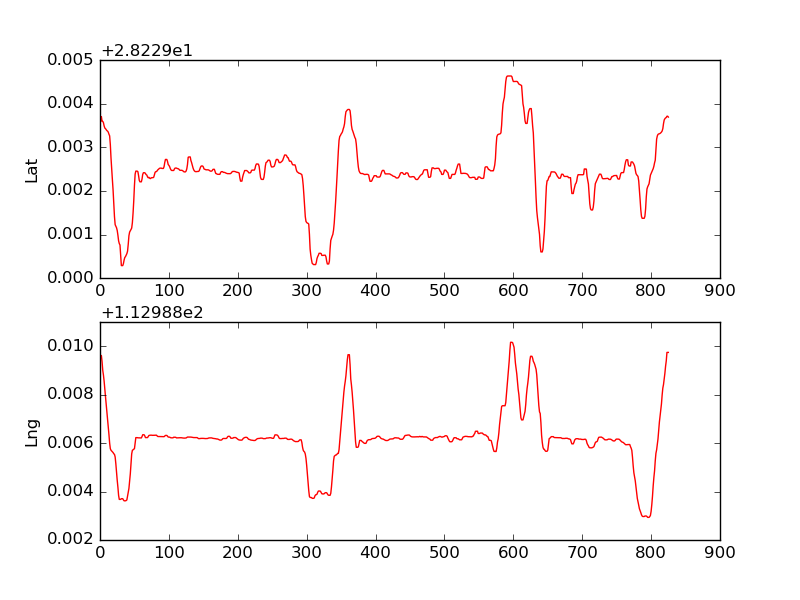
\includegraphics[height=4cm]{figure_4_mid_location2_avg}}
  \caption{轨迹均值滤波实验结果2}
  \label{fig:3_3_2}
\end{figure}
\par 通过对比观察滤波结果图可以发现,相对于中值滤波,均值滤波能够较好的平滑用户的轨迹变化曲线,剔除GPS漂移点。但是,同样无法很有效的处理漂移偏差大的位置点。
\par 通过采取卡尔曼滤波算法得到的用户轨迹如图\ref{fig:3_4_1}、\ref{fig:3_4_2},根据观察图中滤波后的用户轨迹数据,我们可以发现虽然图形变得平滑了许多,但是却使得原有的轨迹信息收到了模糊,难以有效的将两个用户轨迹进行相似度计算。
\begin{figure}[htb]
  \centering%
  \subfloat[原始轨迹数据]{%
    \label{fig:3_2_1_1}
    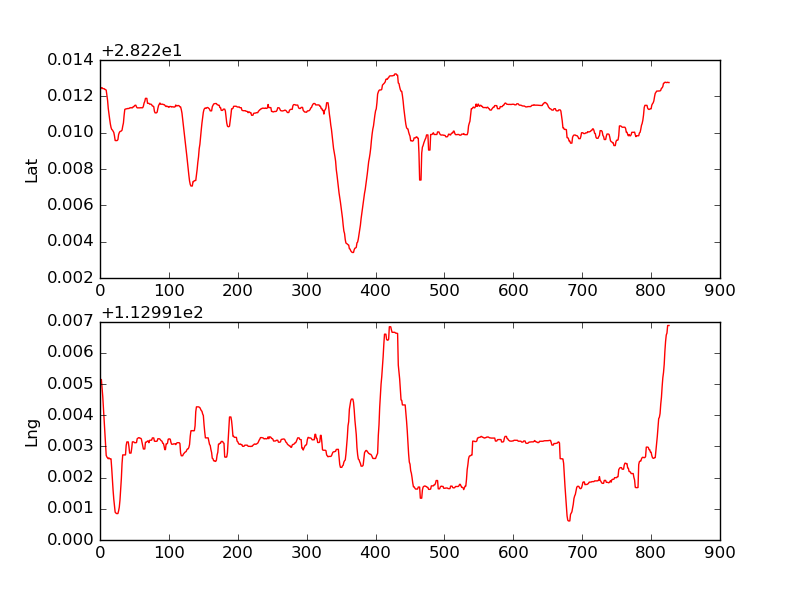
\includegraphics[height=4cm]{figure_4_mid_location1}}\hspace{4em}%
  \subfloat[卡尔曼滤波后的轨迹数据]{%
    \label{fig:3_2_2_1}
    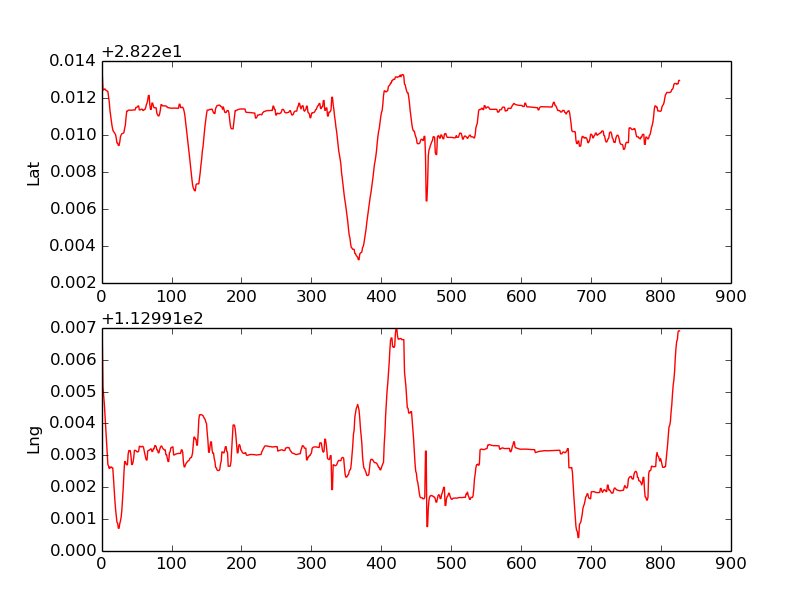
\includegraphics[height=4cm]{figure_4_mid_location1_kalman_ed}}
  \caption{卡尔曼滤波实验结果1}
  \label{fig:3_4_1}
\end{figure}
\begin{figure}[htb]
  \centering%
  \subfloat[原始轨迹数据]{%
    \label{fig:3_2_2_1}
    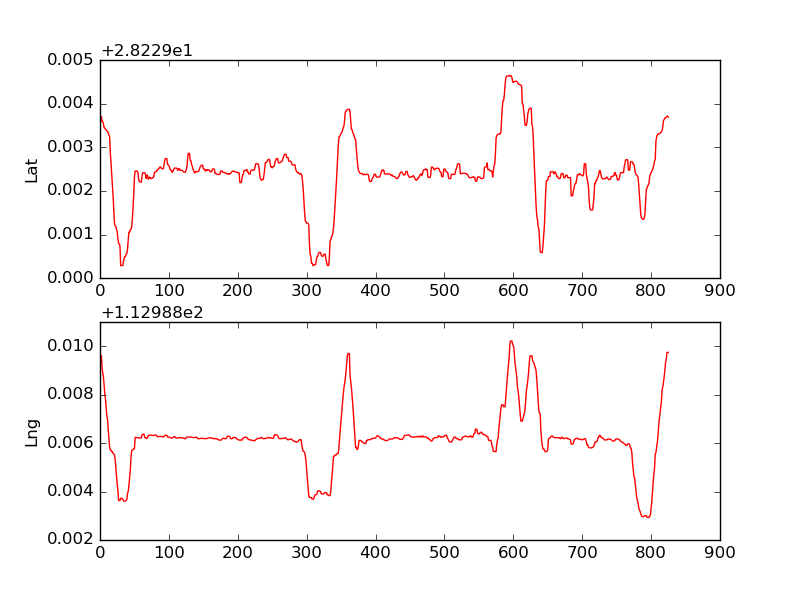
\includegraphics[height=4cm]{figure_4_mid_location2}}\hspace{4em}%
  \subfloat[卡尔曼滤波后的轨迹数据]{%
    \label{fig:3_2_2_2}
    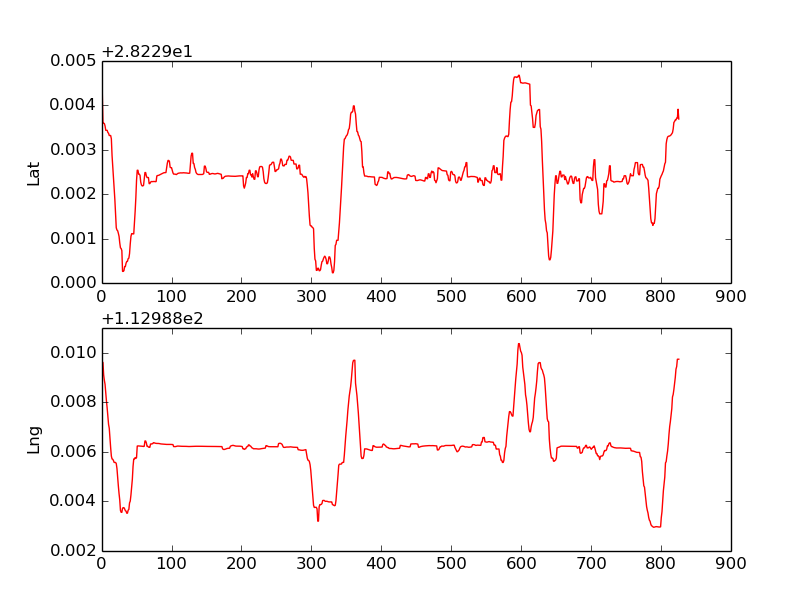
\includegraphics[height=4cm]{figure_4_mid_location2_kalman_ed}}
  \caption{卡尔曼滤波实验结果2}
  \label{fig:3_4_2}
\end{figure}
\par 在本研究中,我们采用了一种基于速度的分段卡尔曼滤波方法。考虑到在一个时间片内,如果当前位置点的速度和它之前的位置点的速度绝对差大于$\Delta v$时($\Delta v$作为一个未知的参数,需要我们在实际使用中给出)采用这样的方法将原有用户轨迹切分为$n$段然后针对每一段轨迹采用卡尔曼滤波算法,最终的部分轨迹滤波结果见图\ref{fig:3_5_1}、\ref{fig:3_5_2},可见经过按照速度分段后使用卡尔曼滤波能够比较好的过滤掉漂移点。
\begin{figure}[htb]
  \centering%
  \subfloat[原始轨迹数据]{%
    \label{fig:3_2_1_1}
    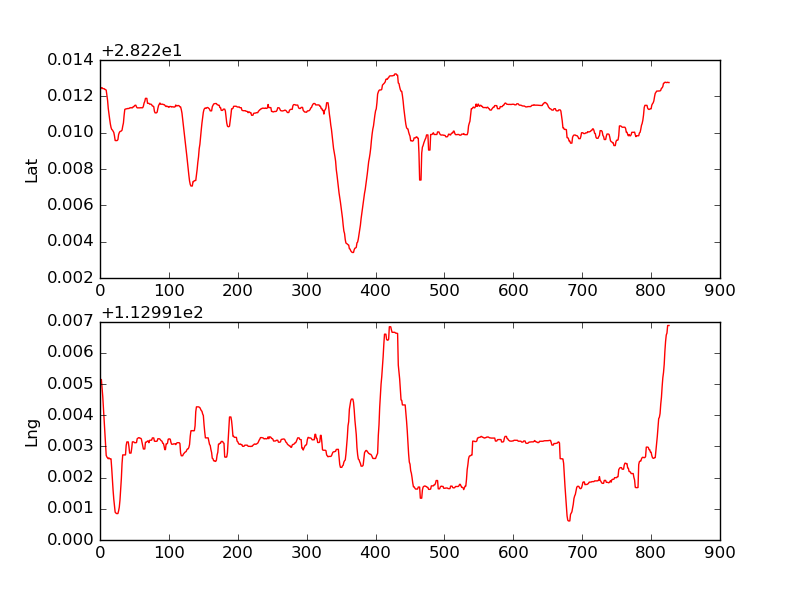
\includegraphics[height=4cm]{figure_4_mid_location1}}\hspace{4em}%
  \subfloat[分段卡尔曼滤波数据]{%
    \label{fig:3_2_2_1}
    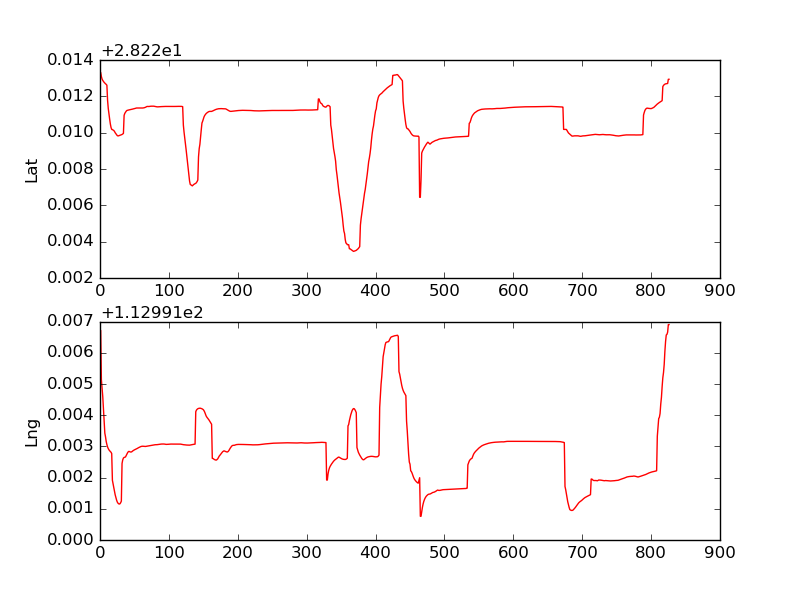
\includegraphics[height=4cm]{figure_4_mid_location1_kalman}}
  \caption{分段卡尔曼滤波轨迹结果1}
  \label{fig:3_5_1}
\end{figure}
\begin{figure}[htb]
  \centering%
  \subfloat[原始轨迹数据]{%
    \label{fig:3_2_2_1}
    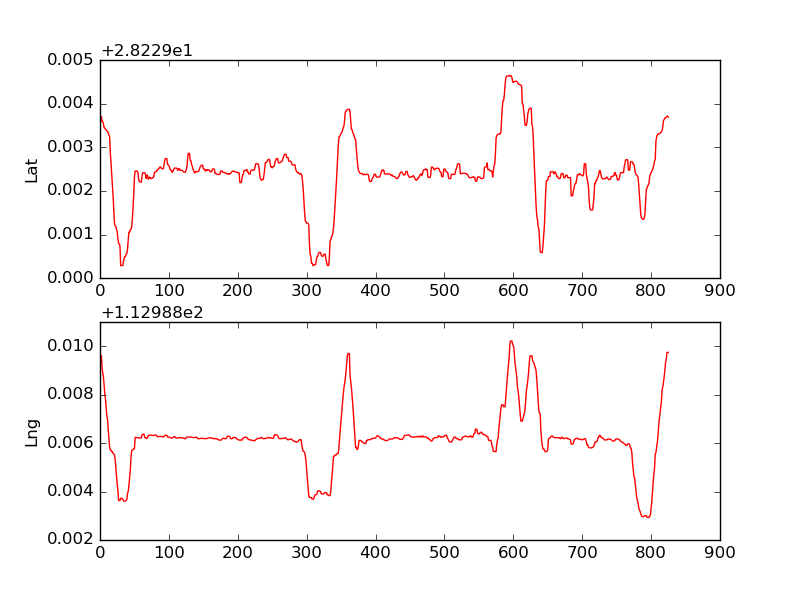
\includegraphics[height=4cm]{figure_4_mid_location2}}\hspace{4em}%
  \subfloat[分段卡尔曼滤波数据]{%
    \label{fig:3_2_2_2}
    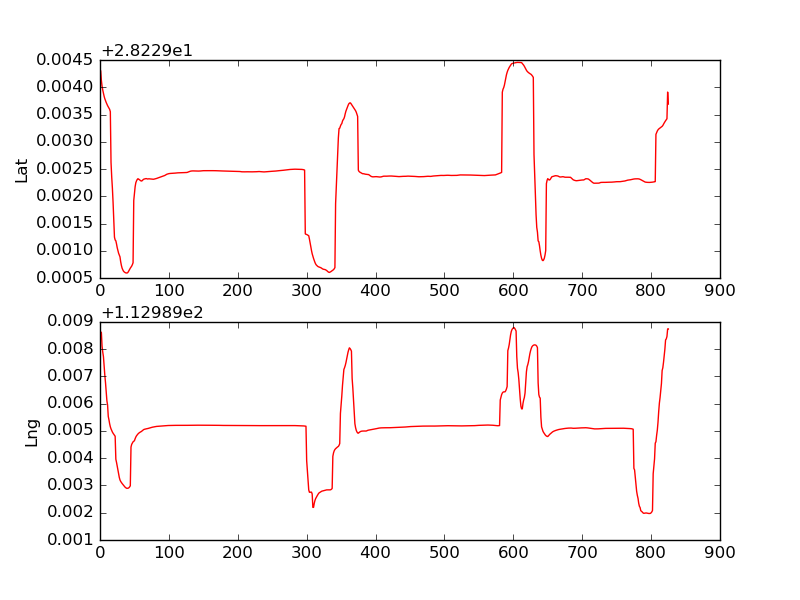
\includegraphics[height=4cm]{figure_4_mid_location2_kalman}}
  \caption{分段卡尔曼滤波轨迹结果2}
  \label{fig:3_5_2}
\end{figure}
\par 本小节主要针对前文中提及的三种常用的滤波算法进行了实验结果展示和效果分析,初步得出了使用卡尔曼滤波更加可行的判断结果。
\subsection{轨迹中停留点检测}
在实际生活中用户的轨迹是由一系列GPS点构成的,剔除其中的噪音点和用户在路上的点,能够从中挖掘出进一步信息的位置信息即为轨迹中的停留点,通常停留点并不是指用户轨迹中速度为零的点,而是由一组GPS 点构成区域,一个停留点通常对应现实生活中富有具体意义的点,能够更好的反映出用户之间轨迹的相似程度。
在现实生活中,人们从一个位置行进到另一个位置是连续的,即采集的数据必然存在很多路上的点。而这些路上的点不属于任何一个语义位置。且在分析关系强度时,如果两个人同时来到同一个语义位置,但是一个从某一个方向过来,而另一个从相反方向过来,虽然这两个人其实在这段时间内待在同一个地方,如果不剔除路上的点,则这两个人的物理位置会受到路上的点的影响,从而使得这两个人轨迹的空间距离反而比较大。在上文讨论的降噪过程中,已经处理了误差比较大的点,因此本节主要讨论如何剔除路上的点。
\par 仔细分析路上的点的特性,发现人们通常在语义位置停留时间比较长,而在路上一直处于移动状态,所以路上点密度通常远远小于语义位置的点的密度。密度定义见公式\ref{equ:chap2:dj-cluster}。且在实际生活中,在路上时通常处于移动状态,设速度为$v$,且每条路每天走的次数也存在上限,设每条路每天最多走$N$ 次,计算密度时采用的半径参数为$R$,设GPS采样频率为$f$。 因为半径参数很小,故可视为在该半径对应圆形区域中行走路线为直线。路上点的密度D存在最大值,计算方法见公式\ref{equ:chap3:density_01}。因此本文采用基于密度的方法剔除异常点。该方法的基本思想为若某个点的密度小于给定阈值,则该点为异常点。通过对日常数据的分析发现,路上点的密度确实远远小于处于语义位置点的密度,见图\ref{figure3_6}。
\begin{figure}[htb]
  \centering%
  \subfloat[原始轨迹数据]{%
    \label{fig:3_3_1_1}
    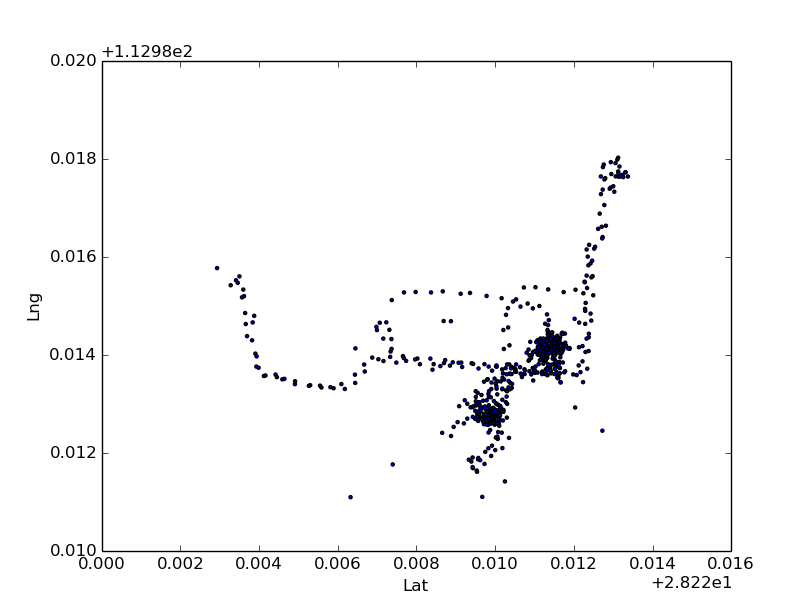
\includegraphics[height=4cm]{figure_4_location1_scater}}\hspace{4em}%
  \subfloat[检测出的停留点]{%
    \label{fig:sp_1}
    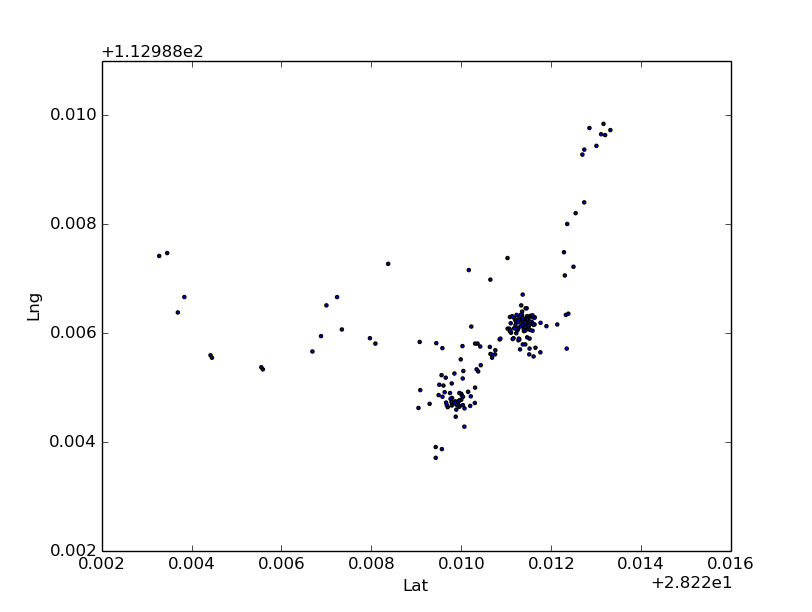
\includegraphics[height=4cm]{figure_4_location1_sp}}
  \caption{停留点检测实验结果1}
  \label{fig:SP_1}
\end{figure}
\begin{figure}[htb]
  \centering%
  \subfloat[原始轨迹数据]{%
    \label{fig:3_3_1_1}
    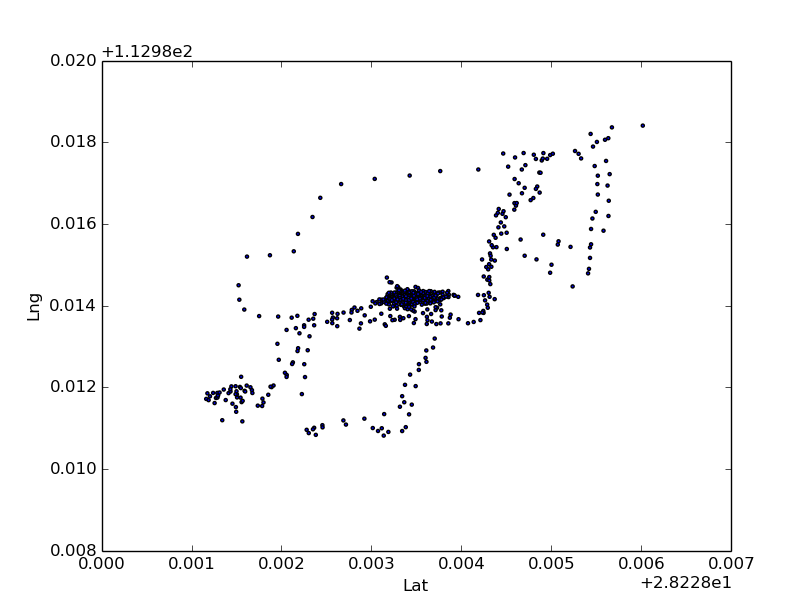
\includegraphics[height=4cm]{figure_4_location2_scater}}\hspace{4em}%
  \subfloat[检测出的停留点]{%
    \label{fig:sp_2}
    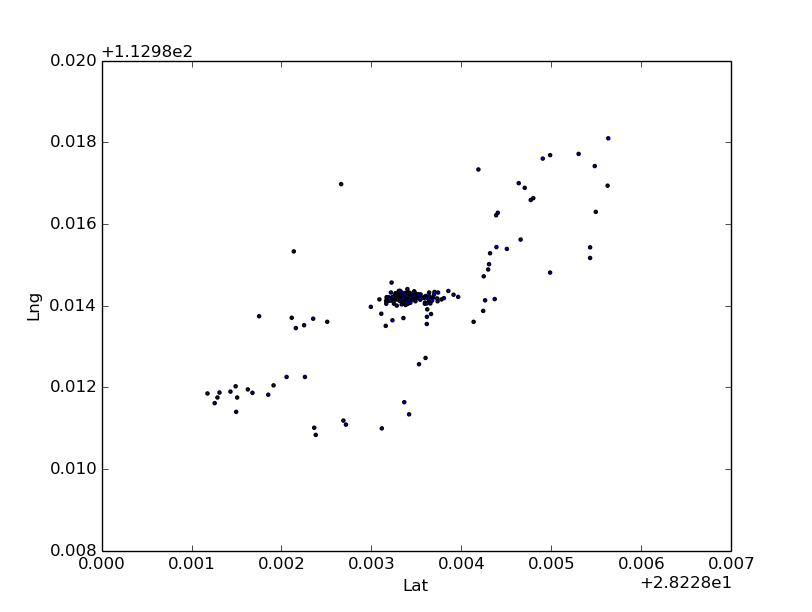
\includegraphics[height=4cm]{figure_4_location2_sp}}
  \caption{停留点检测实验结果2}
  \label{fig:SP_2}
\end{figure}
\par 根据上下文的分析,可以计算出密度的上限值,假设计算密度时的半径设为10米,每天经过这条路4次,步行速度约为80 米每分钟,这样每个点的密度的上限值大概是60。 同时本课题研究发现有一种方法可以自动学习参数,后文将会对比学习到的密度上限值和计算值的异同。
\par 假设对于某一天的数据,已经聚好类,即我们知道哪一个点属于哪一个类别,仔细分析每个路上的点对类别中心的影响,假设用户在某个地方时处于某一个固定的位置,GPS采样因为采样误差服从高斯分布,因此大多数点都处在该固定位置对应实际点(可能是类别中心,非常有可能在类别中心附近)的周围。而路上的点会距离实际点比较远,因此,该类别所有点到类别中心的距离的平均值会被路上的点拉大,如果逐渐提高密度的上限值,从而有更多的点因为密度小而被删除,讨论一种理想情况,如果路上的点完全被剔除,剩下的点都是实际点加高斯误差,因为实际点大量存在,使得即使我们剔除一小部分实际点,对该类别所有点到类别中心的距离的平均值也不会产生太大的影响。所以可以从一个很小的密度上限值逐渐增加,剔除小于该密度的点之后计算对应的平均距离,若平均距离收敛,则认为这个密度值是路上的点的密度的上限值。平均距离的定义见公式\ref{equ:chap3:avgdis_01},其中$p_{ij}$为第$i$类第$j$个点,$c_{i}$为第$i$类的类别中心,$dis(a,b)$表示$a$和$b$之间的距离,$n_{i}$为第$i$类点的个数,$k$为类别的个数,$N$为所有点的个数。使用连续四天采集的数据做了实验,计算其平均距离,见图\ref{fig:3_7}。
\begin{equation}
\label{equ:chap3:avgdis_01}
AvgDis=\frac{\sum_{i=1}^{k}\sum_{j=1}^{n_{i}}dis(p_{ij},c_{i})}{N}
\end{equation}
\begin{figure}[htb]
  \centering%
  \subfloat[第一天数据]{%
    \label{fig:3_7_1}
    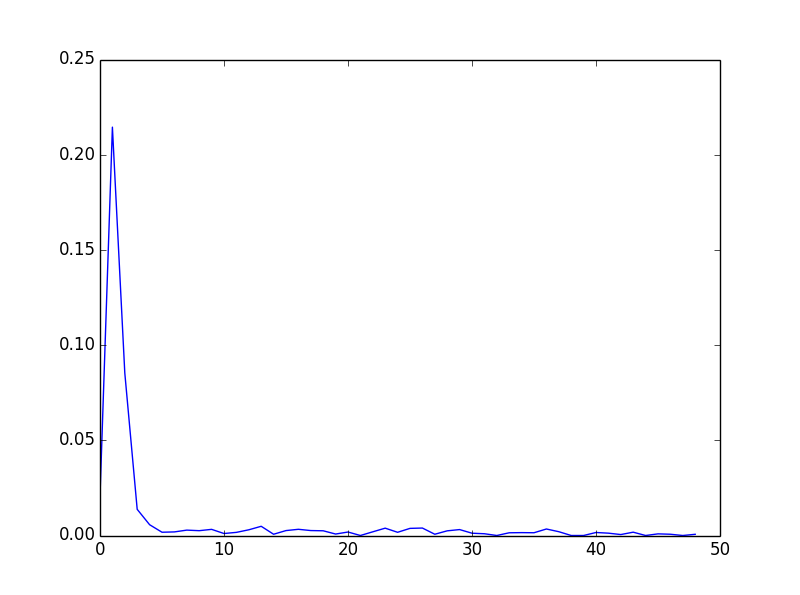
\includegraphics[height=5cm]{figure3_7_1}}%\hspace{4em}
  \subfloat[第二天数据]{%
    \label{fig:3_7_2}
    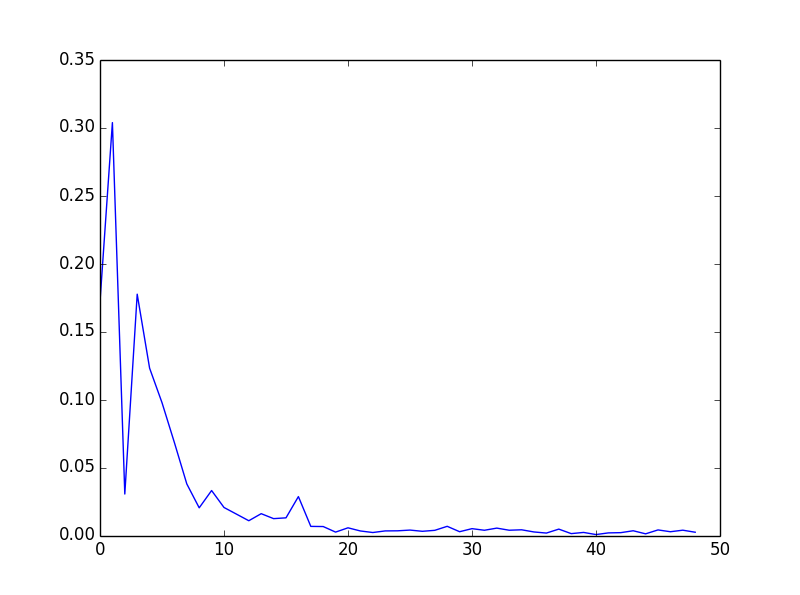
\includegraphics[height=5cm]{figure3_7_2}}\\
  \subfloat[第三天数据]{%
    \label{fig:3_7_3}
    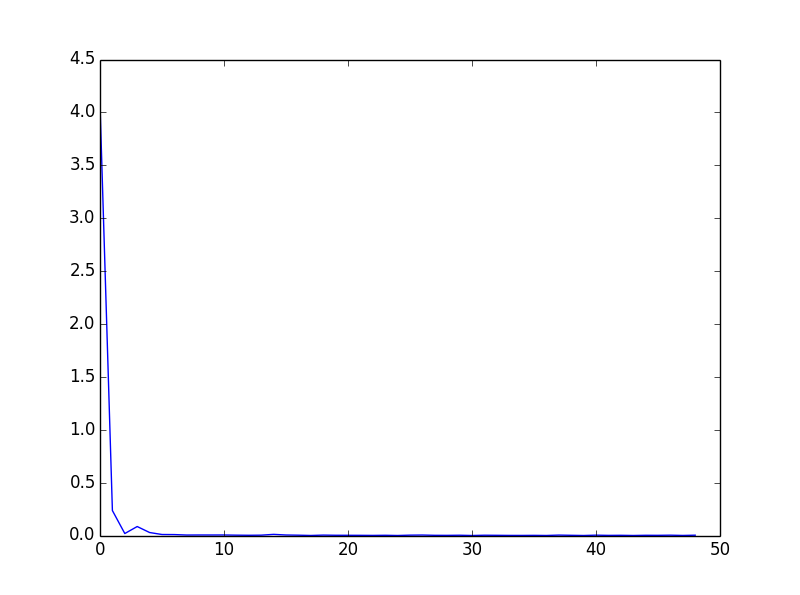
\includegraphics[height=5cm]{figure3_7_3}}
  \subfloat[第四天数据]{%
    \label{fig:3_7_4}
    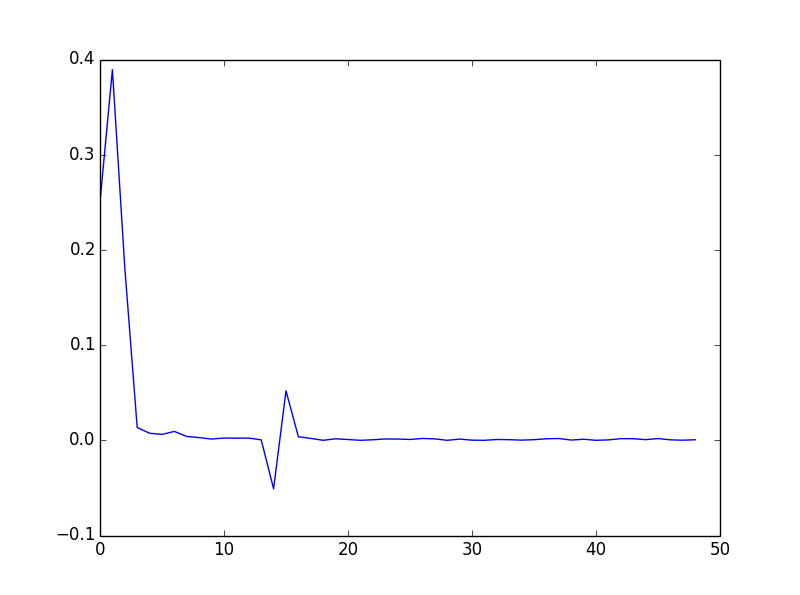
\includegraphics[height=5cm]{figure3_7_4}}
  \caption{平均距离收敛}
  \label{fig:3_7}
\end{figure}
\par 通过观察图\ref{fig:3_7},发现密度上限值大概是40到50之间,前文计算的密度上限值是60左右,一方面因为两种计算方法都存在一定的误差,另一方面是在实际过程中,手机并不是持续高频采样,经常会因为各种各样的原因而丢失一些采样点。在实际应用中,可以先手动处理某一天的数据,然后使用该自动学习的算法学习到密度的上限值,从而用作其他天数据处理的参数。
\par 这一小节主要讨论了如何剔除路上的点,以及如何学习路上点的密度的上限值,下一小节将通过实验讨论K-MEANS、DJ-cluster、以及Science上发表算法三种聚类算法的优缺点,以及在实际数据上应用的效果。
\subsection{聚类得到语义位置}
这一小节将重点描述使用聚类算法得到语义位置时,不同算法以及不同参数对结果产生的影响。K-MEANS、DJ-Cluster以及Science 上发表的三个算法算法原理在第二章已经描述过了,下文将通过实验依次展示三个算法对相同数据聚类得到的结果。数据使用文献\cite{rawassizadeh2013ubiqlog}中的采集工具采集。
\par 首先展示K-MEANS聚类算法的实验结果,K-MEANS聚类算法的主要缺点有两个:一个是需要预知类别的个数;另一个是同一类别的数据最好是团状或簇状。对于本课题研究的问题而言,通常遇到的建筑都是每栋楼占单独的一块地方,相邻建筑一般都会有一定的间隔,因此K-MEANS聚类算法的第二个缺点因为本课题研究的具体问题而不复存在,故主要考虑不同类别个数对实验结果的影响。图\ref{fig:3_8_1}、\ref{fig:3_8_2}、\ref{fig:3_8_3} 主要展示了不同参数对K-MEANS聚类结果的影响。图\ref{fig:3_9_1}、\ref{fig:3_9_2}、\ref{fig:3_9_3}在地图上标记了不同参数聚类得到的聚类中心。
\begin{figure}[htb]
  \centering%
  \subfloat[原始数据]{%
    \label{fig:3_8_1_1}
    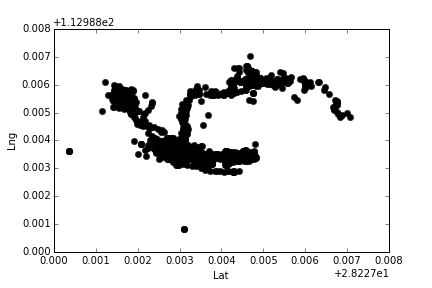
\includegraphics[height=5cm]{figure3_8_1_1}}%\hspace{4em}
  \subfloat[k=3]{%
    \label{fig:3_8_1_2}
    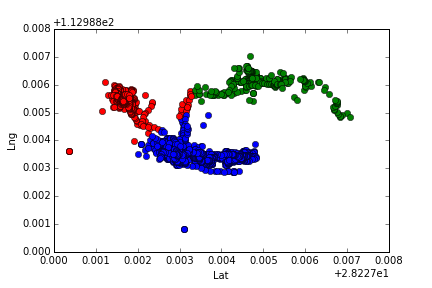
\includegraphics[height=5cm]{figure3_8_1_2}}\\
  \subfloat[k=4]{%
    \label{fig:3_8_1_3}
    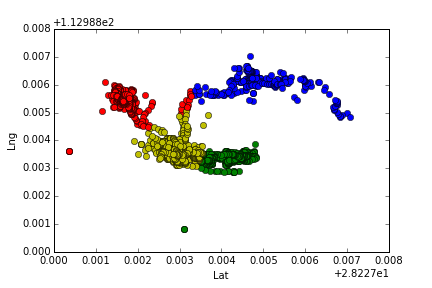
\includegraphics[height=5cm]{figure3_8_1_3}}
  \subfloat[k=5]{%
    \label{fig:3_8_1_4}
    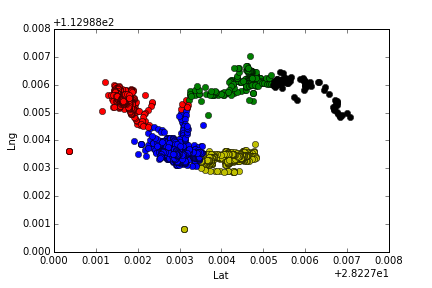
\includegraphics[height=5cm]{figure3_8_1_4}}
  \caption{K-MEANS聚类实验结果3-1}
  \label{fig:3_8_1}
\end{figure}
\begin{figure}[htb]
  \centering%
  \subfloat[原始数据]{%
    \label{fig:3_9_1_1}
    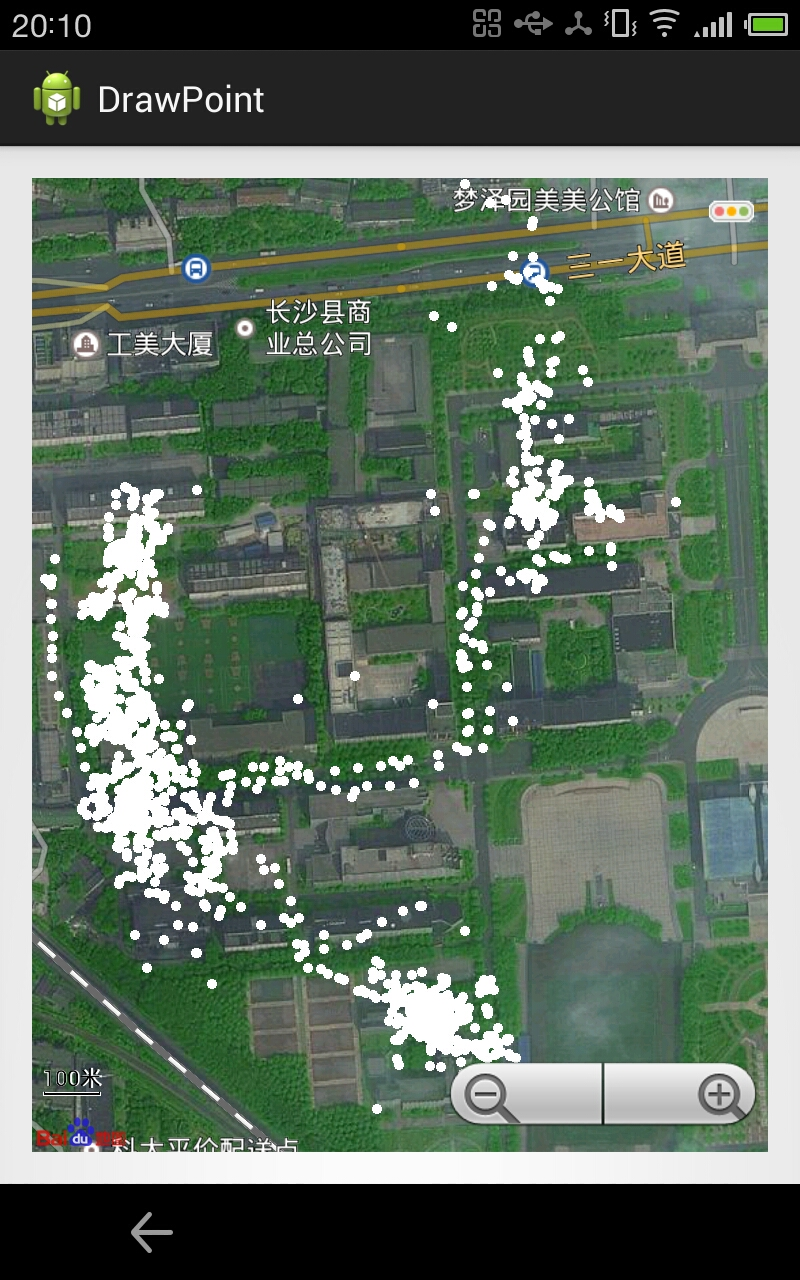
\includegraphics[height=6cm]{figure3_9_1_1}}%\hspace{4em}
  \subfloat[k=3]{%
    \label{fig:3_9_1_2}
    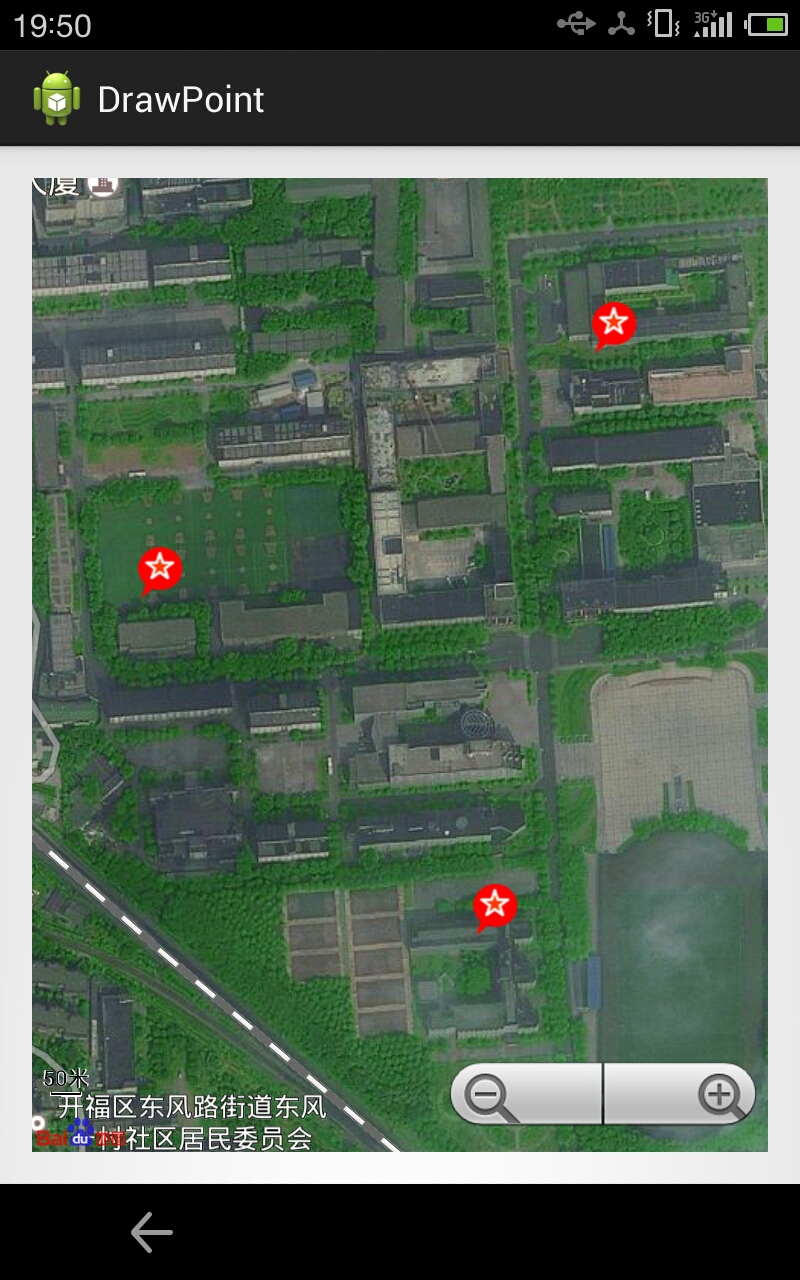
\includegraphics[height=6cm]{figure3_9_1_2}}
  \subfloat[k=4]{%
    \label{fig:3_9_1_3}
    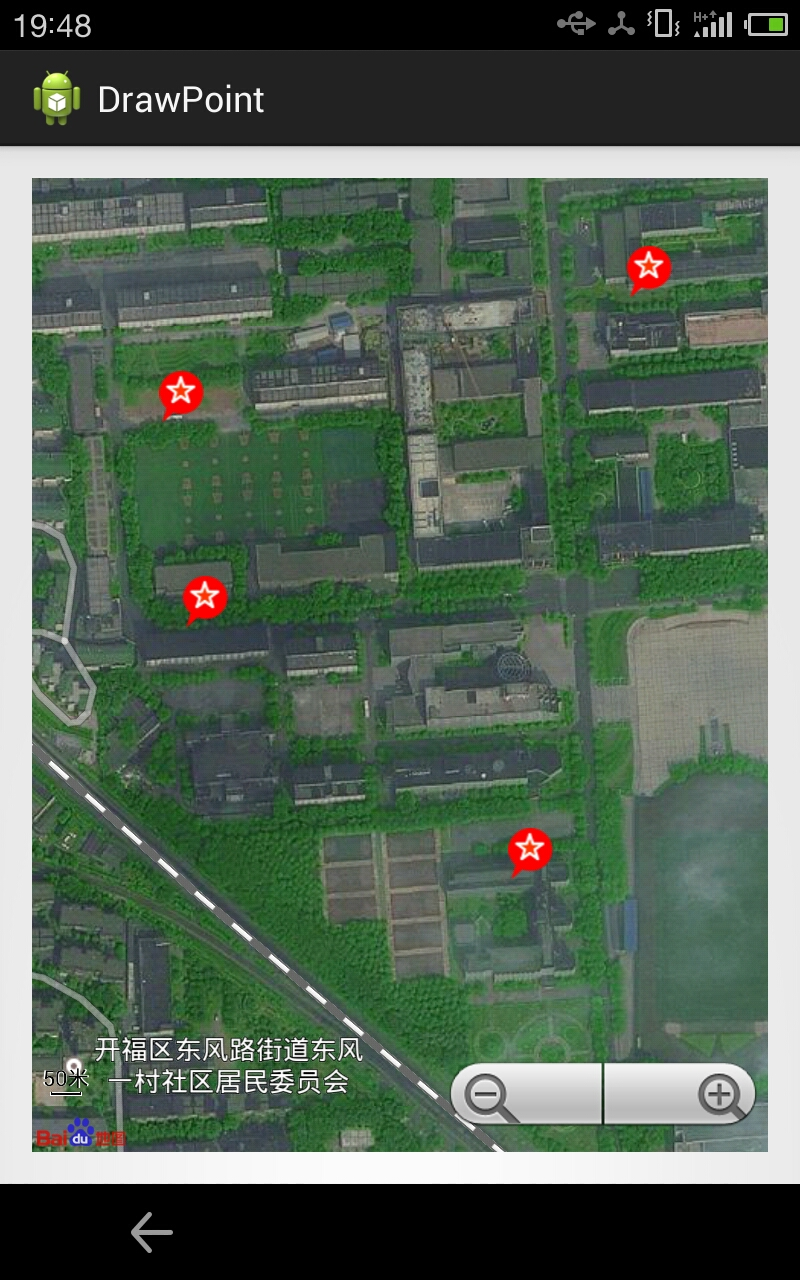
\includegraphics[height=6cm]{figure3_9_1_3}}
  \subfloat[k=5]{%
    \label{fig:3_9_1_4}
    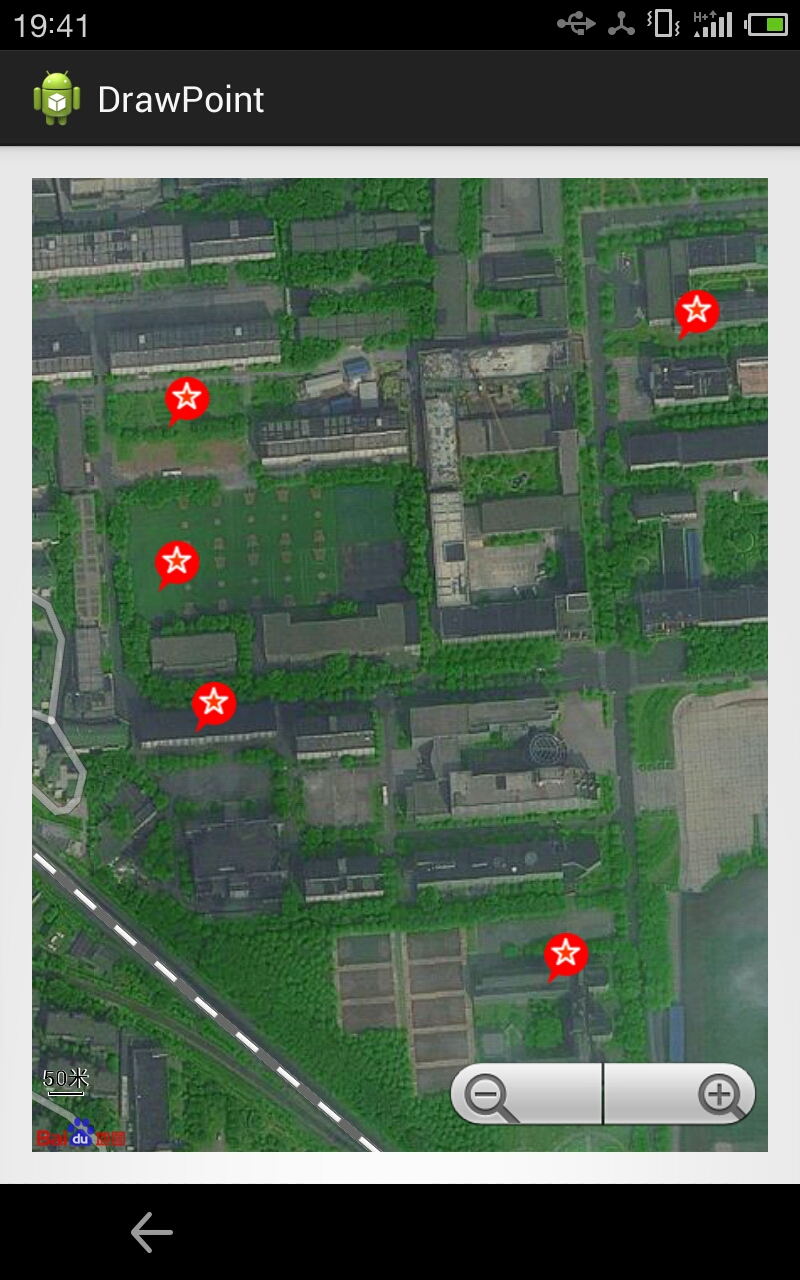
\includegraphics[height=6cm]{figure3_9_1_4}}
  \caption{K-MEANS聚类实验结果地图展示3-1}
  \label{fig:3_9_1}
\end{figure}
\begin{figure}[htb]
  \centering%
  \subfloat[原始数据]{%
    \label{fig:3_8_2_1}
    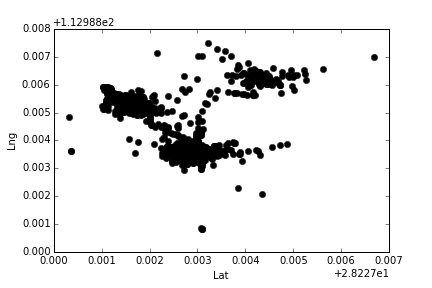
\includegraphics[height=5cm]{figure3_8_2_1}}%\hspace{4em}
  \subfloat[k=3]{%
    \label{fig:3_8_2_2}
    \includegraphics[height=5cm]{figure3_8_2_2}}\\
  \subfloat[k=4]{%
    \label{fig:3_8_2_3}
    \includegraphics[height=5cm]{figure3_8_2_3}}
  \subfloat[k=5]{%
    \label{fig:3_8_2_4}
    \includegraphics[height=5cm]{figure3_8_2_4}}
  \caption{K-MEANS聚类实验结果3-2}
  \label{fig:3_8_2}
\end{figure}
\begin{figure}[htb]
  \centering%
  \subfloat[原始数据]{%
    \label{fig:3_9_2_1}
    \includegraphics[height=6cm]{figure3_9_2_1}}%\hspace{4em}
  \subfloat[k=3]{%
    \label{fig:3_9_2_2}
    \includegraphics[height=6cm]{figure3_9_2_2}}
  \subfloat[k=4]{%
    \label{fig:3_9_2_3}
    \includegraphics[height=6cm]{figure3_9_2_3}}
  \subfloat[k=5]{%
    \label{fig:3_9_2_4}
    \includegraphics[height=6cm]{figure3_9_2_4}}
  \caption{K-MEANS聚类实验结果地图展示3-2}
  \label{fig:3_9_2}
\end{figure}
\begin{figure}[htb]
  \centering%
  \subfloat[原始数据]{%
    \label{fig:3_8_3_1}
    \includegraphics[height=5cm]{figure3_8_3_1}}%\hspace{4em}
  \subfloat[k=3]{%
    \label{fig:3_8_3_2}
    \includegraphics[height=5cm]{figure3_8_3_2}}\\
  \subfloat[k=4]{%
    \label{fig:3_8_3_3}
    \includegraphics[height=5cm]{figure3_8_3_3}}
  \subfloat[k=5]{%
    \label{fig:3_8_3_4}
    \includegraphics[height=5cm]{figure3_8_3_4}}
  \caption{K-MEANS聚类实验结果3-3}
  \label{fig:3_8_3}
\end{figure}
\begin{figure}[htb]
  \centering%
  \subfloat[原始数据]{%
    \label{fig:3_9_3_1}
    \includegraphics[height=6cm]{figure3_9_3_1}}%\hspace{4em}
  \subfloat[k=2]{%
    \label{fig:3_9_3_2}
    \includegraphics[height=6cm]{figure3_9_3_2}}
  \subfloat[k=3]{%
    \label{fig:3_9_3_3}
    \includegraphics[height=6cm]{figure3_9_3_3}}
  \subfloat[k=4]{%
    \label{fig:3_9_3_4}
    \includegraphics[height=6cm]{figure3_9_3_4}}
  \caption{K-MEANS聚类实验结果地图展示3-3}
  \label{fig:3_9_3}
\end{figure}
\par 仔细分析这三组数据的实验结果发现,如果能够预先知道类别的个数,K-MEANS算法确实能够得到一个非常好的结果,特别对于图\ref{fig:3_9_2},仔细观察(a)对应的原始数据,地图右下角白色点群表明其实去了两个教学楼,但是两个教学楼距离太近以及GPS本身存在的采样误差使得采样点混合在一起。如果假设去了三个地方时,该聚类算法将两个教学楼识别成了一个位置,如果假设去了四个地方时,聚类算法成功的区分了这两个实验楼,在另外两个算法的实验中将发现,另外两个算法无法区分这两个实验楼。对于图\ref{fig:3_9_1},其实只参观了三个地方,但是如果假设去了四个地方,该聚类算法也能将数据分成四类,仔细观察得到第四个类别其实是两条路的交叉点,从另一个角度证明前文论述应该剔除路上的点是非常合理的,而后文的实验也证明剔除路上的点之后,聚类算法就不会再把路上的点识别成聚类中心。
\par 下文将展示DJ-Cluster算法的实验结果,DJ-Cluster是基于DBSCAN算法的一种基于密度的聚类算法,通过边界点将相邻类别合并从而使得算法对参数更加鲁棒。但是算法本身仍然严重依赖半径值和密度值这两个参数,在实际应用过程中,仍然需要仔细调节参数,在参数设置理想的情况下,仍然能够得到非常理想的结果,见图\ref{fig:3_10_1}、\ref{fig:3_10_2}、\ref{fig:3_10_3},其地图表示见图\ref{fig:3_11_1}、\ref{fig:3_11_2}、\ref{fig:3_11_3}。
\begin{figure}[htb]
  \centering%
  \subfloat[原始数据]{%
    \label{fig:3_10_1_1}
    \includegraphics[height=4cm]{figure3_8_1_1}}\hspace{4em}%
  \subfloat[聚类结果]{%
    \label{fig:3_10_1_2}
    \includegraphics[height=4cm]{figure3_10_1_2}}
  \caption{DJ-Cluster实验结果3-1}
  \label{fig:3_10_1}
\end{figure}
\begin{figure}[htb]
  \centering%
  \subfloat[原始数据]{%
    \label{fig:3_11_1_1}
    \includegraphics[height=6cm]{figure3_9_1_1}}\hspace{4em}%
  \subfloat[聚类结果]{%
    \label{fig:3_11_1_2}
    \includegraphics[height=6cm]{figure3_11_1_2}}
  \caption{DJ-Cluster实验结果地图表示3-1}
  \label{fig:3_11_1}
\end{figure}
\begin{figure}[htb]
  \centering%
  \subfloat[原始数据]{%
    \label{fig:3_10_2_1}
    \includegraphics[height=4cm]{figure3_8_2_1}}\hspace{4em}%
  \subfloat[聚类结果]{%
    \label{fig:3_10_2_2}
    \includegraphics[height=4cm]{figure3_10_2_2}}
  \caption{DJ-Cluster实验结果3-2}
  \label{fig:3_10_2}
\end{figure}
\begin{figure}[htb]
  \centering%
  \subfloat[原始数据]{%
    \label{fig:3_11_2_1}
    \includegraphics[height=6cm]{figure3_9_2_1}}\hspace{4em}%
  \subfloat[聚类结果]{%
    \label{fig:3_11_2_2}
    \includegraphics[height=6cm]{figure3_11_2_2}}
  \caption{DJ-Cluster实验结果地图表示3-2}
  \label{fig:3_11_2}
\end{figure}
\begin{figure}[htb]
  \centering%
  \subfloat[原始数据]{%
    \label{fig:3_10_3_1}
    \includegraphics[height=4cm]{figure3_8_3_1}}\hspace{4em}%
  \subfloat[聚类结果]{%
    \label{fig:3_10_3_2}
    \includegraphics[height=4cm]{figure3_10_3_2}}
  \caption{DJ-Cluster实验结果3-3}
  \label{fig:3_10_3}
\end{figure}
\begin{figure}[htb]
  \centering%
  \subfloat[原始数据]{%
    \label{fig:3_11_3_1}
    \includegraphics[height=6cm]{figure3_9_3_1}}\hspace{4em}%
  \subfloat[聚类结果]{%
    \label{fig:3_11_3_2}
    \includegraphics[height=6cm]{figure3_11_3_2}}
  \caption{DJ-Cluster实验结果地图表示3-3}
  \label{fig:3_11_3}
\end{figure}
\par 通过对实验结果的分析能够发现,DJ-Cluster基本上能够得到一个令人满意的结果,在仔细调节参数后,基本上识别出了所有的位置,但是图\ref{fig:3_11_2}右下角其实是两个教学楼,前文已经论述过,DJ-Cluster 将其识别为一个位置,主要是因为这两个教学楼本身距离太小,且GPS采样误差比较大使得本来分属于两栋楼的采样点有重合,从而使得基于密度的方法无法区分。除此情况外,对于另外两天的数据,该算法都表现出了非常好的识别结果。该算法最大的缺陷还是对参数比较敏感,下文将介绍Science 发表的聚类算法的实验结果,同时会从算法原理上简要论述其对参数的鲁棒性确实优于DJ-Cluster。
\par 下文描述Science发表的聚类算法对应的实验结果,在描述具体实验之前,首先分析该算法的原理:该算法对每个点计算对应的密度(密度定义见前文),对所有点按密度排序;然后计算每个点的距离,再对每个点按距离和密度的乘积排序得到最终的聚类结果。DJ-Cluster算法之所以对参数敏感是因为不同的半径值就需要对应不同的密度值(半径大了,此半径对应的圆形区域内其他点的数目肯定会更多),而Science发表的算法会对所有点按密度排序,这样在很大程度上降低了半径值对算法本身的影响,通常情况下半径越大点密度越大,如果随着半径的增长,密度的相对顺序保持不变,则半径对该算法基本没有影响,本课题收集的GPS 采样点基本满足这一条件,若某个点在小半径时密度小,则在大半径是其密度依然相对较小。所以Science发表的算法对当前问题而言有非常好的鲁棒性。具体的实验结果见图\ref{fig:3_12_1}、\ref{fig:3_12_2}、\ref{fig:3_12_3}。实验结果地图表示见图\ref{fig:3_13_1}、\ref{fig:3_13_2}、\ref{fig:3_13_3}。
\begin{figure}[htb]
  \centering%
  \subfloat[原始数据]{%
    \label{fig:3_12_1_1}
    \includegraphics[height=4cm]{figure3_8_1_1}}\hspace{4em}%
  \subfloat[聚类结果]{%
    \label{fig:3_12_1_2}
    \includegraphics[height=4cm]{figure3_12_1_2}}
  \caption{Science发表算法实验结果3-1}
  \label{fig:3_12_1}
\end{figure}
\begin{figure}[htb]
  \centering%
  \subfloat[原始数据]{%
    \label{fig:3_13_1_1}
    \includegraphics[height=6cm]{figure3_9_1_1}}\hspace{4em}%
  \subfloat[聚类结果]{%
    \label{fig:3_13_1_2}
    \includegraphics[height=6cm]{figure3_13_1_2}}
  \caption{Science发表算法实验结果地图表示3-1}
  \label{fig:3_13_1}
\end{figure}
\begin{figure}[htb]
  \centering%
  \subfloat[原始数据]{%
    \label{fig:3_12_2_1}
    \includegraphics[height=4cm]{figure3_8_2_1}}\hspace{4em}%
  \subfloat[聚类结果]{%
    \label{fig:3_12_2_2}
    \includegraphics[height=4cm]{figure3_12_2_2}}
  \caption{Science发表算法实验结果3-2}
  \label{fig:3_12_2}
\end{figure}
\begin{figure}[htb]
  \centering%
  \subfloat[原始数据]{%
    \label{fig:3_13_2_1}
    \includegraphics[height=6cm]{figure3_9_2_1}}\hspace{4em}%
  \subfloat[聚类结果]{%
    \label{fig:3_13_2_2}
    \includegraphics[height=6cm]{figure3_13_2_2}}
  \caption{Science发表算法实验结果地图表示3-2}
  \label{fig:3_13_2}
\end{figure}
\begin{figure}[htb]
  \centering%
  \subfloat[原始数据]{%
    \label{fig:3_12_3_1}
    \includegraphics[height=4cm]{figure3_8_3_1}}\hspace{4em}%
  \subfloat[聚类结果]{%
    \label{fig:3_12_3_2}
    \includegraphics[height=4cm]{figure3_12_3_2}}
  \caption{Science发表算法实验结果3-3}
  \label{fig:3_12_3}
\end{figure}
\begin{figure}[htb]
  \centering%
  \subfloat[原始数据]{%
    \label{fig:3_13_3_1}
    \includegraphics[height=6cm]{figure3_9_3_1}}\hspace{4em}%
  \subfloat[聚类结果]{%
    \label{fig:3_13_3_2}
    \includegraphics[height=6cm]{figure3_13_3_2}}
  \caption{Science发表算法实验结果地图表示3-3}
  \label{fig:3_13_3}
\end{figure}
\par 仔细分析由Science发表算法对应的实验结果发现,其结果和DJ-Cluster的结果基本完全一致,图\ref{fig:3_13_2}、其实有四个地方,该算法也只识别出来三个,未能正确识别的原因如前文所述,其对另外两天的数据都能全部识别出来。其算法的鲁棒性在前文已经论述过了,在此讨论与该算法相关的另外一个参数,即密度和距离乘积的阈值。原论文中声明他们的算法不需要任何手动设置任何参数,但是经过实验发现该阈值仍然需要通过观察具体数据集的特性来确定。虽然不能完全不需要人的参与,通过实验发现对于特定的数据集,比如采集的校园内的GPS数据,通过对第一天数据的分析,能够得到一个密度和距离乘积的阈值,通过实验发现该阈值对后面采集的数据依然有效,即只需要在刚开始使用该算法时确定该参数,就可以使用该参数处理其他剩余的数据。这样在很大程度上减少了人与机器的交互,使得该算法更加实用。
\par 这一小节主要讨论了三种聚类算法以及不同的参数对实验结果的影响。最后讨论对每天数据进行聚类的优缺点。以前的工作都是采集一段时间的数据,把所有数据合并到一起,然后用这些聚类算法来计算对应的语义位置。最明显的一个问题是如果聚类结果表明这些数据总共产生了1000 个位置(如果是K-MEANS 算法需要预先设定类别的个数),那么这些数据是否恰好对应1000个语义位置。这样做的优点是处理方便,只需要一次交互,缺点是计算结果无法验证。当然,主要是因为移动感知这个领域目前对结果精度要求也不是很高,但是有没有什么办法在不明显增加处理复杂度的同时使得结果更加精确?因此本课题决定对每天的数据进行聚类,一方面小数据更容易精确识别,如果用户总共去了三个地方,可能识别出来两个,则只有一个没有识别出来,而没事别出来的那个可能因为下文论述的原因被重新发现,如果把所有数据一起处理,假设总共参观了100个地方,可能只识别出来70几个,另外20 多个无法被识别;另一方面如果每个地方因为当天采集数据太少而未被识别,用户下一次去这个地方且采集数据较多时就会被重新识别出来,对最终结果来说,仍然正确识别了这个地方。而且小数据量使得在移动端计算成为可能,可以将整个过程全部放在手机上,而不影响用户体验。在识别出这些位置后下一步需要标记其语义标签,将大量的数据分散到每天,且通过识别新的位置以及对新位置计算可能的语义标签在很大程度上降低了用户与手机的交互,下一节将详细讨论如何在发现语义位置后对其标记对应的语义标签。
\section{对语义位置标语义标签}
\label{sec:section3-3}
在上一节主要描述了如何对GPS数据进行滤波以达到降噪的目的、如何剔除路上的点以及如何使用聚类算法得到语义位置。仅仅得到语义位置的信息是不够的,如果只是知道这个用户在什么时候去了一个地方,但是并不知道这个地方是什么(一般指该地方的功名称)。如果能够得到这个地方的语义信息,则能够解决更多的问题。如果知道一个人从早到晚一整天都在实验室,只使用这些信息就可以确定,这个人很大可能是博士。而且根据用户经常停留的位置也可以从健康角度提一些建议,如果某用户整天在室内办公,就可以提醒他应该抽出一定的时间去室外锻炼。因此,确定语义位置对应的语义标签是非常重要的一个问题。本节主要介绍如何确定语义位置对应的语义标签。
\subsection{发现新位置}
一般通过两种方法来得到语义位置对应的语义标签。一种方法是预先定义几种语义标签,使用监督学习的方法学习出一个分类器模型,然后对未知标签的数据通过用分类器分类得到其对应的语义标签。该方法的优点是结果比较准确,有坚实的理论基础做支撑,而且只有在收集数据时需要用户参与;缺点是需要大量的数据来训练模型,训练模型需要大量的时间,且只能识别预定义的几种语义标签,对新的语义标签无能为力。另外一种方法是首先通过聚类算法识别出用户参观过的所有的语义位置,然后在地图上标记出来,人工标记语义位置对应的语义标签。该方法的优点是可以不断处理新的位置;缺点是需要用户的参与,影响用户体验。
\par 无法预先确定全部的语义标签,只能采用第二种方法来获取可能的语义标签。但是在处理过程中仍然采取了很多措施来降低用户和手机的交互。前文已经论述了对每天采集数据进行处理的原因。在每天用户睡觉前(这种情况下通常手机充电且已连接WIFI)对当天采集的数据进行处理,聚类得到当天去过的语义位置,为了减少用户和手机的交互,在得到语义位置之后会判断今天有没有新的位置,用户只需要对新去过的位置标记语义标签,这一小节将主要描述如何发现新的语义位置。在得到新的语义位置后会通过一定的方法来计算可能的语义标签以减少用户与手机的交互,下一小节将重点描述如何计算可能的语义标签。
\par 为了减少用户与手机的交互,在用户标记语义标签时,只标记新位置的语义标签,如果某个位置已经标记了对应的语义标签,则当该位置再次出现时,将直接忽略该位置。
\par 发现新位置最重要的问题在于,即使对于同一个语义位置,因为采样的误差使得计算得到的聚类中心不一定完全相同。首先设计一个已标记表,记录用户已经参观过的语义位置及其对应的语义标签,以及该位置参观过的次数。每次计算得到一个语义位置时,计算该位置与已标记表中每一个位置之间的距离,若该位置和与其最近的位置之间的距离小于某一个给定阈值比如说20米,则认为该位置和与其最近的位置是一个位置。虽然这两个位置是同一个位置,但是这两个位置在数值上并非完全相同,因此尝试通过一定的方法来修正该实际位置的数值。把与该实际位置是同一个位置的所有已经参观过的位置的平均值作为该实际位置新的数值表示,见公式\ref{equ:chap3:avggps_01}。这也是在已标记表中需要记录参观该位置次数的原因。
\begin{equation}
\label{equ:chap3:avggps_01}
avgLat = (avgLat\ast n+newLat)/(n+1),avgLng = (avgLng\ast n+newLng)/(n+1)
\end{equation}
\par 然而并未完全解决该问题,最主要问题是一个位置和另一个位置到底距离多近才可以将其视为一个位置。发现新位置的实验会在下一节和计算可能的语义标签一起展示,在实际应用过程中,对于小数据量,相对来说还是可以得到一个比较精确的结果,但是对于大数据量,可靠性很难得到保证。而且该方法非常依赖聚类算法的结果,而聚类算法的结果又非常依赖实际采集到的数据,实际采数据的过程无法控制,因此聚类算法的结果也很难控制。猜想每天同一个位置采集的数据聚类得到的聚类中心是不是也服从一定的分布,如果通过实验数据能够确定该分布,通过参数估计就可以得到实际位置一个更可靠的估计值。这也是下一步的工作之一。
\subsection{新位置语义标签提示}
上一小节讨论了如何发现新位置,这一节将详细讨论如何计算新位置可能的语义标签。本课题主要通过三种方式来减少用户和手机之间的交互:第一种方法是采用简单的推断方法来推断该新位置可能的语义标签;第二种方法是利用当前电子地图提供的获取反地理编码的接口来获取当前位置对应的反地理编码作为当前位置的语义标签;第三种方法是在用户输入时提供自动补全功能,减少用户的参与。
\par 首先描述简单推断方法。综合考虑手机的计算能力以及算法的可靠性,决定采用基于规则的方法来推断新位置可能的语义标签,这也意味着只能得到一些比较简单的结果,而不能像常用的分类算法那样可以处理很多种语义标签的情况,可以视为性能和精确度之间的一个权衡。
\par 考虑最简单的两种语义标签家和办公室(实验室)。之所以称其为最简单的语义标签是因为这两个语义标签对应的语义位置有着非常明显的特点,比如家通常是夜间停留一整晚的地方,而办公室通常是白天停留一整天的地方,这些特点使得这两个地方和其他地方有非常大的区别,从而可以使用一些很简单的规则把他们和其他地方区分开。具体处理方法如下。
\par 先描述如何推断家这个语义标签。对零点到早上七点这段时间内出现的语义位置分别计算在其对应的地方停留的时间,并计算该时间相对于七个小时占的百分比。若这段时间内只有一个语义位置,且其时间占到了总时间93\% 以上(之所以不是100\% 是因为采样存在误差,若误差比较大会被视为异常点从而使得对停留时间的统计出现偏差,选择93\%是因为可以有半个小时的偏差)则认为这个语义位置对应的语义标签是家,否则就把这个语义位置当做一个新的位置用剩下的方法去猜测可能的语义标签。
\par 然后描述如何推断办公室这个语义标签。按照一般情况下朝九晚五的规定,对早上九点到中午十二点,下午一点到下午五点这七个小时内出现的语义位置分别计算在其对应的地方停留的时间,并计算该时间相对于七个小时所占的百分比。中间有一个小时被忽略掉是因为猜测通常情况下这一个小时大家应该是出去吃午饭。剩下处理步骤与推断家这个语义标签的处理完全相同。这样就能够很简单的得到新位置是不是家或者实验室。该方法一般情况下都能取得比较理想的结果,见图\ref{fig:3_14}。该方法可能存在的一个问题是,第一天的数据中,用户晚上并未睡在自己家里,这样就可能导致一个误判,但是仔细分析我们的处理过程,这一步只是计算可能的语义标签,最后仍然需要用户的确认,所以即使推断错了也不会影响最终的语义标签。
\begin{figure}[htb]
  \centering%
  \subfloat[推断宿舍]{%
    \label{fig:3_14_1}
    \includegraphics[height=6cm]{figure3_14_1}}%\hspace{4em}%
  \subfloat[推断实验室]{%
    \label{fig:3_14_2}
    \includegraphics[height=6cm]{figure3_14_2}}
  \subfloat[语义标签地图示意]{%
    \label{fig:3_14_3}
    \includegraphics[height=6cm]{figure3_14_3}}
  \caption{语义标签推断结果示意}
  \label{fig:3_14}
\end{figure}
\par 下面主要描述通过反地理编码获取语义位置对应的语义标签。在此之前需要先描述一下诸如百度地图、高德地图之类的电子地图以及这些地图提供的接口。百度地图是百度提供的一项网络地图搜索服务,覆盖了国内近400个城市、数千个区县。同时百度地图提供编程接口,我们可以通过对地图接口的调用得到全景图展现,热力图展示,定制个性地图,地图2D、3D、卫星图的展示,本地检索,周边检索,区域检索,公交检索,驾车检索、覆盖物,反\/地理编码,实时交通等功能。本课题主要使用反地理编码功能。反地理编码实现地址解析服务,具体是指从已知的经纬度坐标到对应的地址描述(如省市、街区、楼层、房间等)的转换服务。
\par 反地理编码只能返回一些比较大的地方的语义标签,对于实验室、教学楼、图书馆这种地方依然无能为力,这时候就需要用户手动输入来标记这些地方的语义标签。手动输入时为了减少用户的交互采用了安卓自己提供的文本框输入自动补全功能。见图\ref{fig:3_15}。
\begin{figure}[htb]
  \centering%
  \subfloat[推断宿舍]{%
    \label{fig:3_15_1}
    \includegraphics[height=6cm]{figure3_15_1}}%\hspace{4em}%
  \subfloat[推断实验室]{%
    \label{fig:3_15_2}
    \includegraphics[height=6cm]{figure3_15_2}}
  \subfloat[语义标签地图示意]{%
    \label{fig:3_15_3}
    \includegraphics[height=6cm]{figure3_15_3}}
  \caption{语义标签推断结果示意}
  \label{fig:3_15}
\end{figure}
\par 到目前为止展示了计算可能语义标签的三种方法,也得到了一个相对理想的结果,但是这个处理过程仍然太简单,还有很多问题需要解决,这也是下一步的工作。
\section{小结}
\label{sec:section3-4}
本章主要描述了一些对GPS数据额外的处理,这些处理方法在第五章准备轨迹数据时有用。本章首先描述了使用均值滤波、中值滤波、卡尔曼滤波以及分段卡尔曼滤波的实验结果,发现分段卡尔曼滤波能够获得一个更理想的结果;之后描述了使用K-MEANS、DJ-Cluster以及Science发表聚类算法三种聚类算法发现语义位置的实验结果以及分析了各种算法的优缺点;在获得语义位置的基础上描述了如何对语义位置标记对应的语义标签,先计算新的位置,然后计算新位置可能的语义标签,并且展示了实验结果。下一章将描述提出的度量用户关系强度的URSHV计算方法以及实验验证。
\chapter{用户关系强度计算方法}
\label{chap:chapter04}
在上一章详细描述了面向GPS数据的语义标签标注技术,这一章重点描述我们自己提出的URSHV用户关系强度计算方法。将从计算方法概述、输入数据准备以及关系强度计算三方面来描述URSHV计算方法。
\section{用户关系强度计算方法概述}
\label{sec:section4-1}
层级用户关系度量计算方法URSHV从三个不同的抽象层次,从不同角度采用不同的方法来度量用户之间的关系强度。第一层基于用户日常的原始轨迹数据度量用户日常轨迹之间的相似度;第二层度量的是基于语义位置的用户行为模式之间的相似度,其抽象层次比第一层更高,其含义比第一层更加丰富;第三层度量的是基于语义标签的用户行为模式之间的相似度,其抽象层次比第二层更高,语义更加精确。URSHV模型从轨迹、物理位置以及语义位置等三个由低到高的抽象层次,从三个反映人们日常活动和行为模式的方面来度量人们之间的关系强度,并基于这三个层次的度量结果,采用集成学习的思想进行投票,以投票结果作为人们之间的关系强度,因而能够全面真实地反映日常生活当中人们之间的关系强度。
\begin{figure}[htp]
\centering
\includegraphics[height=6cm]{figure4_1}
\caption{URSHV模型框架}
\label{fig:4_1}
\end{figure}

\section{输入数据准备}
\label{sec:section4-2}
上一节概述了计算方法,这一节将具体描述如何对GPS数据和基站数据进行预处理以得到需要的输入,下一节将具体描述如何计算用户之间的关系强度。
\par 在日常生活中,用户的位置既可以通过智能手机内嵌的GPS传感器获取其位置信息,又可以通过用户所处区域内的通信基站进行定位。通过GPS获取的位置信息相对与通过基站获取的位置信息要精确,但是长时间通过GPS传感器采集用户的位置信息将消耗大量的电量,会对用户手机的日常使用造成一定的影响。虽然基于基站的定位方式相对于GPS定位方式获取的位置信息精度要低,但其更有利于用户隐私的保护。因此,为了满足不同用户的不同需求,URSHV模型既能够对GPS位置数据进行处理,同时又能够对基站位置数据进行处理。但是,无论是基于GPS的位置数据还是基于通信基站的位置数据都包含着大量的噪音,因此,为了更加精确地度量用户之间的关系强度,我们首先对这些数据进行去噪处理,而后采用不同方法来计算用户之间的关系强度。
\par 设用户集合为$U$,$U=\{u_{1},u_{2},...,u_{n}\}$,其中$n$表示用户个数,$D_{i}$表示用户$u_{i}$采集数据的日期的集合,表示为$D_{i}=\{d_{1},d_{2},...,d_{m_{i}}\}$,其中$m_{i}$表示用户$u_{i}$采集数据的总天数。$F_{i}$表示用户$u_{i}$ 的全部朋友组成的集合,表示为$F_{i}=\{u_{k_{1}},u_{k_{2}},...,u_{k_{f_{i}}}\}$,其中$f_{i}$表示用户$u_{i}$ 的好友的个数。$Trace$ 表示所有用户所有天的轨迹数据的集合,表示$Trace=\{Trace_{1},Trace_{2},...,Trace_{n}\}$,其中$Trace_{i}$ 表示用户$u_{i}$所有天采集的轨迹序列的集合,表示为$Trace_{i}=\{Trace_{i,k}|k\in D_{i}\}$。$Trace_{i,k}$ 表示用户$u_{i}$ 在$k$ 这一天的轨迹序列,表示为$Trace_{i,k}=\{l_{1},l_{2},...,l_{n_{i,k}}\}$,其中$n_{i,k}$表示用户$u_i$在$k$ 这一天采集的轨迹数据的条数,$l_b$表示$b$时刻采集的位置数据记录,可以为GPS经纬度,也可以是基站号。
\par 对于GPS数据和基站数据表示的用户轨迹序列进行预处理时,我们在下面三小节中分别依次描述模型的三层输入。
\subsection{轨迹数据的处理与准备}
处理GPS数据:对每个用户每天的数据$Trace_{i,k}$进行滤波,目的是减少数据噪声;对每个用户每天的数据按半个小时进行切割,即将用户$u_{i}$的每天数据$Trace_{i,k}$ 按时间均分为$48$份,表示为$Sep\_trace_{i,k}=\{Sep\_trace_{i,k,1},...,Sep\_trace_{i,k,48}\}$,其中每一份数据表示为$Sep\_trace_{i,k,s}=\{l_{a_i}|l_{a_i}\in Trace_{i,k} \bigwedge a_{i} \in s\}$;对$Sep\_trace_{i,k,s}$ 按经纬度计算平均值,并将新的轨迹序列表示为$Ntrace_{i,k}$,$Ntrace_{i,k}=\{Ntrace_{i,k,1},...,\\
Ntrace_{i,k,48}\}$,其中$Ntrace_{i,k,s}=\frac{sum(Sep\_trace_{i,k,s})}{len(Sep\_trace_{i,k,s})}$;其中$sum(A)$表示对序列A中的元素求和,$len(A)$表示序列$A$的长度。将$Ntrace_{i}$作为用户$u_{i}$使用第一层算法计算其与全部好友关系强度的输入。
\par 处理基站数据: 对每个用户每天的数据按半个小时进行切割,即将用户$u_{i}$在$k$这一天的数据$Trace_{i,k}$按时间均分为$48$份,表示为$Sep\_trace_{i,k}=\{Sep\_trace_{i,k,1},...,Sep\_trace_{i,k,48}\}$,其中每一份数据表示为$Sep\_trace_{i,k,s}=\{l_{a_i}|l_{a_i}\in Trace_{i,k}\bigwedge a_{i}\in s\}$;对每半个小时内数据计算依次不重复的基站号序列,即对每一份数据计算其对应的集合$set(Sep\_trace_{i,k,s})$,确保基站号不重复;再将每天$48$份数据重新拼成一个序列,目的是对每天轨迹序列降维,否则计算量太大而实际无法计算,新序列记为$Ntrace_{i,k}$。其中$Ntrace_(i,k)=\bigcup_{s=1}^{48}set(Sep\_trace_{i,k,s})$;将$Ntrace_{i}$作为用户$u_{i}$使用第一层算法的输入。
\subsection{语义位置数据的处理与准备}
GPS数据准备:采用上一章中讨论的聚类方法对所有用户的轨迹数据进行聚类,得到全部语义位置表示为$Loc=\{pl_{1},...,pl_{g}\}$,其中$g$ 表示总共的语义位置的个数。通过聚类得到用户$u_{i}$在$k$这一天的语义位置序列表示为$Ltrace_{i,k}=\{loc(l_{1}),loc(l_{2}),...,loc(l_{n_{i,k}})\}$,其中$loc(l_{j})$表示位置数据记录$l_{j}$对应的语义位置标号。所有用户的所有语义位置序列表示为$Ltrace=\{Ltrace_{1},...,Ltrace_{n}\}$,其中用户$u_{i}$的全部语义位置序列表示$Ltrace_{i}=\{Ltrace_{i,k}|k\in D_{i}\}$。对每个用户每天的数据按半个小时进行切割,即将用户$u_{i}$的每天数据$Ltrace_{i,k}$按时间均分为$48$份,表示为$Sep\_ltrace_{i,k}=\{Sep\_ltrace_{i,k,1},...,Sep\_ltrace_{i,k,48}\}$,其中每一份数据表示为$Sep\_ltrace_{i,k,s}=\{loc(l_{a_{i}})|l_{a_{i}}\in Trace_{i,k}\bigwedge a_{i}\in s\}$。在准备word2vec 模型的输入数据以及对应的模型输入数据时:我们需要首先计算每份数据不重复的语义位置序列,即$Lsep\_ltrace_{i,k,s}=set(Sep\_ltrace_{i,k,s})$,然后将每天的$48$ 分数据合并成一个序列得到$LLtrace$,$LLtrace_{i,k}=\bigcup_{s=1}^{48}Lsep\_ltrace_{i,k,s}$。将$LLtrace$作为word2vec模型的输入,训练得到对应模型$LW2V(M)$,$M$表示每个语义位置对应的实数值向量的长度。将$Lsep\_ltrace_{i}$作为用户$u_{i}$在第二层使用word2vec 模型计算关系强度时的输入。其中$Lsep\_ltrace_{i,k}=\{Lsep\_ltrace_{i,k,1},...,Lsep\_ltrace_{i,k,48}\}$。在准备LDA 模型的输入数据以及对应的模型输入数据时:在已得到$Sep\_ltrace$的基础上,对每份数据计算不重复出现的语义位置,并对每个位置加上时间标记。用户$u_{i}$在$k$这一天第$s$时间段语义位置序列表示为$Tltrace_{i,k,s}=\{TT(sl_{b})|sl_b\in set(Sep\_ltrace_{i,k,s})\}$,其中$TT(sl_{b})$表示对$sl_{b}$添加时间标记,表示该语义位置在该时间段出现。$set(A)$表示计算序列$A$对应的集合,即$A$中无重复元素。将$Tltrace_{i}$作为用户$u_{i}$在第二层算法使用LDA模型计算关系强度时的输入。将$Tltrace_{i,k}$中的$48$份数据合并成一个序列$LTltrace$,其中$LTltrace_{i,k}=\bigcup_{s=1}^{48}Tltrace_{i,k,s}$ 。将$LTltrace$ 作为LDA模型的输入,训练得到对应的LDA主题模型$LLDA(K)$,$K$表示主题的个数。
\par 基站数据准备:将每一个基站视为一个物理位置,即Ltrace=Trace。其余处理与GPS处理完全相同。
\subsection{语义标签数据的处理与准备}
GPS数据准备:对前文得到的$Loc$中每一个语义位置采用上一章中讨论的方法标记其语义标签,标语义标签后用户$u_{i}$第$k$天的语义标签序列表示为$Strace_{i,k}=\{Label(ll_{b})|ll_{b}\in ltrace_{i,k}$,其中$Label(ll_{b})$表示$ll_{b}$对应的语义标签。所有用户的所有语义标签序列表示为$Strace=\{Strace_{1},...,Strace_{n}\}$,其中用户$u_{i}$的全部语义位置序列表示$Strace_{i}=\{Strace_{i,k}|k\in D_{i}\}$。 对每个用户每天的数据按半个小时进行切割,即将用户$u_{i}$的每天数据$Strace_{i,k}$按时间均分为$48$份,表示为$Sep\_strace_{i,k}=\{Sep\_strace_{i,k,1},...,Sep\_strace_{i,k,48}\}$,其中每一份数据表示为$Sep\_strace_{i,k,s}=\{Label(l_{a_{i}})|l_{a_{i}}\in Ltrace_{i,k} \bigwedge a_{i}\in s\}$。在准备word2vec 模型的输入数据以及对应的模型输入数据时:我们需要首先计算每份数据不重复的语义标签序列,即$Ssep\_strace_{i,k,s}=set(Sep\_strace_{i,k,s})$,然后将每天的$48$份数据合并成一个序列得到$SLtrace$,$SLtrace_{i,k}=\bigcup_{s=1}^{48}Ssep\_strace_{i,k,s}$。将$SLtrace$作为word2vec模型的输入,训练得到对应模型$SW2V(M)$,$M$表示每个语义位置对应的实数值向量的长度。将$Ssep\_strace_{i}$作为用户$u_{i}$在第三层使用word2vec 模型计算关系强度时的输入。其中$Ssep\_strace_{i,k}=\{Ssep\_strace_{i,k,1},...,Ssep\_strace_{i,k,48}\}$。在准备LDA 模型的输入数据以及对应的模型输入数据时:在已得到$Sep\_strace$的基础上,对每份数据计算不重复出现的语义位置,并对每个位置加上时间标记。用户$u_{i}$在$k$这一天第$s$时间段物理位置序列表示为$Tstrace_{i,k,s}=\{TT(sl_{b})|sl_{b}\in set(Sep\_strace_{i,k,s})\}$,其中$TT(sl_{b})$表示对$sl_{b}$ 添加时间标记,表示该语义位置在该时间段出现。$set(A)$表示计算序列$A$对应的集合,即$A$中无重复元素。将$Tstrace_{i}$作为用户$u_{i}$在第三层算法使用LDA模型计算关系强度时的输入。将$Tstrace_{i,k}$中的$48$份数据合并成一个序列$STstrace$,其中$STstrace_{i,k}=\bigcup_{s=1}^{48}Tstrace_{i,k,s}$ 。将$STstrace$ 作为LDA模型的输入,训练得到对应的LDA主题模型$SLDA(K)$,$K$表示主题的个数。
\par 基站数据准备:计算每一个基站对应的语义标签,其余处理与GPS数据处理完全相同。
\par 准备好模型各个层次的输入数据后,在下一节我们将详细描述如何使用输入数据计算用户之间的关系强度。
\section{关系强度计算}
\label{sec:section4-3}
上一节我们描述了如何准备模型对应的三层输入数据,这一节我们将分别描述基于轨迹数据的关系强度计算方法和基于主题模型的关系强度计算方法。
\subsection{基于原始轨迹数据的关系强度计算}
我们计算每一个用户$u_{i}$与其每一个朋友$u_{k}(u_{k}\in F_{i})$之间的关系强度,并对$F_{i}$中的每一个朋友,按照其与$u_{i}$的关系强度大小按降序排列,使此序列中任意两个朋友与$u_{i}$的关系强弱顺序尽可能与实际情况一致。
\par 基于DTW及序列熵值加权计算用户之间的关系强度。对用户$u_{i}$的每一个好友$u_{k}$,利用上一小节得到的$Ntrace_{i}$ 和$Ntrace_{k}$计算其轨迹序列相似度。$Ntrace_{i,a}$表示用户$i$在$a$这一天的数据,其中$a\in D_{i}$,$Ntrace_{k,b}$表示用户$k$在$b$这一天的数据,其中$b\in D_{k}$。$S(i,j)$表示若$a=b$则取值为1,否则取值为0。$DTW(Ntrace_{i,a},Ntrace_{k,b})$表示用户$u_{i}$在$a$这一天的轨迹和用户$u_{k}$在$b$ 这一天的轨迹的相似度, $Entropy(Ntrace_{i,a})$表示用户$u_{i}$在$a$这一天的轨迹序列的熵值。则用户$u_{i}$和用户$u_{k}$的基于轨迹序列的关系强度计算方法见公式\ref{equ:chap4:dtw}。DTW计算的是距离,距离越小相似度越大,即该公式值越小,两个用户关系强度越强。
\begin{equation}
\label{equ:chap4:dtw}
Ent_Dtw(u_{i},u_{k})=\frac{1}{\sum_{a\in D_{i},b\in D_{k}}S(a,b)}\sum_{a\in D_{i},b\in D_{k}}S(a,b)\frac{DTW(Ntrace_{i,a},Ntrace_{k,b})}{Entropy(Ntrace_{i,a})}
\end{equation}
\subsection{基于主题模型的关系强度计算}
LDA模型对应的关系强度计算方法:$Tltrace_{i}$表示用户$u_{i}$根据上一小节得到的语义位置序列,$Tltrace_{k}$表示用户$u_{k}$根据上一小节得到的语义位置序列。$T(a,p,b,q)$表示若用户$u_{i}$在$a$这一天第$p$个时间段和用户$u_{k}$在$b$这一天第$q$个时间段数据均存在则为1,否则为0。$LLDA(K).inf(Tltrace_{i,a,p})$表示对$Tltrace_{i,a,p}$推断得到的主题分布,通常表示为$K$维的向量,其中$K$表示主题的个数。基于用户语义位置的行为模式的关系强度计算方法见公式\ref{equ:chap4:llda},其中$cos$表示余弦相似度。
\begin{equation}
\label{equ:chap4:llda}
\begin{split}
&LocLDA(u_{i},u_{k})=\frac{1}{\sum_{a\in D_{i},b\in D_{k}}S(a,b)}\sum_{a\in D_{i},b\in D_{k}}S(a,b)\frac{1}{\sum_{p=q=1}^{48}T(a,p,b,q)}\\
&\sum_{p=q=1}^{48}T(a,p,b,q)\ast cos⁡(LLDA(K).inf(Tltrace_{i,a,p} ),LLDA(K).inf(Tltrace_{k,b,q}))\\
\end{split}
\end{equation}
\par 基于用户语义标签的行为模式的关系强度计算公式与基于语义位置的关系强度计算公式相似,见公式\ref{equ:chap4:slda}。
\begin{equation}
\label{equ:chap4:slda}
\begin{split}
&SemLDA(u_{i},u_{k})=\frac{1}{\sum_{a\in D_{i},b\in D_{k}}S(a,b)}\sum_{a\in D_{i},b\in D_{k}}S(a,b)\frac{1}{\sum_{p=q=1}^{48}T(a,p,b,q)}\\
&\sum_{p=q=1}^{48}T(a,p,b,q)\ast cos⁡(SLDA(K).inf(Tstrace_{i,a,p}),SLDA(K).inf(Tstrace_{k,b,q}))\\
\end{split}
\end{equation}
\par word2vec模型对应的关系强度计算方法:$Lsep\_strace_{i}$表示用户$u_{i}$根据上一小节得到的语义位置序列,$Lsep\_strace_{k}$表示用户$u_{k}$根据上一小节得到的语义位置序列。$T(a,p,b,q)$表示若用户$u_{i}$ 在$a$这一天第$p$个时间段和用户$u_{k}$在$b$这一天第$q$个时间段数据均存在则为1,否则为0。$DTW(Lsep\_strace_{i,a,p},Lsep\_strace_{k,b,q})$表示$Lsep\_strace_{i,a,p}$和$Lsep\_strace_{k,b,q}$之间的DTW距离。计算DTW距离时需要知道两个语义位置之间的距离,我们用这两个语义位置对应的实数值向量之间的余弦距离作为这两个语义位置之间的距离。即由用户语义位置的行为模式得到的关系强度计算方法见公式\ref{equ:chap4:lw2v}。
\begin{equation}
\label{equ:chap4:lw2v}
\begin{split}
&LocW2V(u_{i},u_{k})=\frac{1}{\sum_{a\in D_{i},b\in D_{k}}S(a,b)}\sum_{a\in D_{i},b\in D_{k}}S(a,b)\frac{1}{\sum_{p=q=1}^{48}T(a,p,b,q)}\\
&\sum_{p=q=1}^{48}T(a,p,b,q)\ast DTW(Lsep\_strace_{i,a,p},Lsep\_strace_{k,b,q})\\
\end{split}
\end{equation}
\par 基于用户语义标签的行为模式的关系强度计算公式与基于语义位置的关系强度计算公式相似,见公式\ref{equ:chap4:sw2v}。
\begin{equation}
\label{equ:chap4:sw2v}
\begin{split}
&SemW2V(u_{i},u_{k})=\frac{1}{\sum_{a\in D_{i},b\in D_{k}}S(a,b)}\sum_{a\in D_{i},b\in D_{k}}S(a,b)\frac{1}{\sum_{p=q=1}^{48}T(a,p,b,q)}\\
&\sum_{p=q=1}^{48}T(a,p,b,q)\ast DTW(Ssep\_strace_{i,a,p},Ssep\_strace_{k,b,q})\\
\end{split}
\end{equation}
\par 我们更关注的是用户和好友A的关系强度大于或小于用户与好友B的关系强度。因此我们实际计算结果为用户与其全部好友按关系强度降序排列得到的好友序列。
\subsection{结果投票}
对于用户$u_{i}$,我们对其全部好友$F_{i}$中的每一个朋友$u_{k}$使用$Ent_DTW(u_{i},u_{k})$计算用户$u_{i}$和用户$u_{k}$之间的关系强度,并对$F_{i}$中的每一个朋友按照计算得到的关系强度降序排列得到$E_{i}=\{u_{d_{1}},...,u_{d_{f_{i}}}\}$,其中$Ent_DTW(u_{i},u_{d_{a}})>Ent_DTW(u_{i},u_{d_{b}})$如果$a<b$。在此基础上,我们使用$LocLDA(u_{i},u_{k})$或者$LocW2V(u_{i},u_{k})$ 计算用户$u_{i}$和用户$u_{k}$ 之间的关系强度,并对$F_{i}$中的每一个朋友按照计算得到的关系强度降序排列得到$L_{i}=\{u_{l_{1}},...,u_{l_{f_{i}}}\}$,其中$LocLDA(u_{i},u_{l_{a}})>LocLDA(u_{i},u_{l_{b}})$或者$LocW2V(u_{i},u_{l_{a}})>LocW2V(u_{i},u_{l_{b}})$如果$a<b$。 最后我们使用$SemLDA(u_{i},u_{k})$或者$SemW2V(u_{i},u_{k})$计算用户$u_{i}$ 和用户$u_{k}$之间的关系强度,并对$F_{i}$ 中的每一个朋友按照计算得到的关系强度降序排列得到$S_{i}=\{u_{s_{1}},...,u_{s_{f_{i}}}\}$,其中$SemLDA(u_{i},u_{l_{a}})>SemLDA(u_{i},u_{l_{b}})$或者$SemW2V(u_{i},u_{l_{a}})>SemW2V(u_{i},u_{l_{b}})$如果$a<b$。 我们采用集成学习的思想对三个层次的计算结果$E_{i}$、$L_{i}$、$S_{i}$ 进行投票,投票规则为:对于与用户$u_{i}$关系第$k$强的好友$u_{v_{k}}$($k\leq 1$且$k\ll f_{i}$),我们使用三个层次对应的方法分别计算得到$u_{d_{k}}$、$u_{l_{k}}$ 和$u_{s_{k}}$,若这三个用户都不相同,则我们认为$u_{v_{k}}=u_{d_{k}}$,若某个用户比如$u_{l_{k}}=u_{s_{k}}$出现两次及以上,我们认为$u_{v_{k}}=u_{l_{k}}$。以$V_{i}=\{u_{v_{1}},...,u_{v_{f_{1}}}\}$作为投票的最终结果。
\section{小结}
\label{sec:section4-4}
本章就如何使用轨迹数据度量用户之间的关系强度进行了深入讨论,首先描述了URSHV的计算方法,该方法能同时处理GPS数据和基站数据,并使用轨迹数据计算用户之间的关系强度;其次我们从GPS数据和基站数据两方面描述了如何准备URSHV的输入数据;最后我们从基于轨迹数据计算用户关系强度和基于用户行为模式计算用户关系强度两方面详细描述了我们如何使用轨迹数据度量用户之间的关系强度。下一章我们将主要描述实验用到的数据集,评估方法以及在数据集上的实验结果。
\chapter{数据集、评估方法及实验结果}
\label{chap:chapter03}
上一章我们首先概括描述了URSHV层级模型;然后描述了如何准备数据作为模型的输入;最后从基于原始轨迹数据的用户关系强度计算、基于主题模型的用户关系强度计算以及结果投票三方面重点描述了基于轨迹数据的用户关系强度度量模型。本章我们将描述如何在真实数据集上对第四章提出的模型进行验证以及对实验结果进行分析。
\section{数据集}
\label{sec:section5-1}
我们采用真实场景下采集的数据作为验证数据集。数据集由MIT媒体实验室在2004-2005年主持的RealityMining项目收集整理得到。RealityMining 项目追踪了94个使用安装预装软件的手机的用户,这些预装软件能够记录并发送用户数据,比如:通话记录、近似5米范围内的蓝牙设备、基站塔编号、应用使用以及手机状态。该项目追踪观察了包括学生和来自同一个研究机构的两个课题组的职员总共九个月对手机的使用情况。与此同时,该项目收集了每个志愿者提供的关系数据比如谁和谁是朋友等。
\par 每个志愿者使用Nokia6600在后台运行一个称为ContextLog的程序采集数据。在该项目中期,研究者组织了一次在线调查问卷,106 个志愿者中共有94 个人完成了该调查问卷。调查问卷内容见表\ref{tab:questionnaire}。 除此调查问卷外,采集的数据有每个志愿者手机的蓝牙MAC地址、每个志愿者开始参与该项目的日期、每个志愿者隶属的机构、每个志愿者隶属的研究小组、每个志愿者收集的IMEI、 每个志愿者的邻居、每个志愿者自己告知的工作时间、每个志愿者是否有一个规律的工作计划、每个志愿者自己告知的常去的聚集地、每个志愿者是否有一个可预言的日程安排、每个志愿者是不是把手机忘在家里或工作的地方、每个志愿者手机电量是不是经常耗光、每个志愿者生病频率、每个志愿者最近是否生病、每个志愿者是否经常出去旅游、给每个志愿者提供通话服务的运营商、每个用户每个月购买东西花费的时间、每个志愿者发短信的频率、每个志愿者是否经常被描述给其他人、每个治愈者对他所处团体的评价、每个志愿者的通信时间记录、每个志愿者收集充电记录、每个志愿者收集使用日期记录、每个志愿者手机采集数据的记录时间、每个志愿者开机关机时间记录、每个志愿者的轨迹数据记录(由基站号、区域号以及时间戳构成)、用户经过的唯一的位置(由基站号和区域号表示)、每个志愿者周围的蓝牙设备名称、每个志愿者周围的蓝牙设备的MAC地址、每个志愿者扫描周围蓝牙设备的时间、基站号及区域号对应的位置语义标签、每个志愿者使用应用的开始时间及使用时长、每个志愿者手机每天记录数据的时长、每个志愿者家对应的基站号和区域号扥等。基站号及区域号与对应的语义标签见表\ref{tab:baseSemantic}。
\begin{longtable}[l]{l*{1}{l}}
\caption{调查问卷\upcite{eagle2006reality}}\label{tab:questionnaire}\\
\toprule[1.5pt]
 问题及答案选项
%\midrule[1pt]%
\endfirsthead%

\multicolumn{1}{l}{续表-调查问卷}\\
\toprule[1.5pt]
 问题及答案选项
%\midrule[1pt]%
\endhead%
\hline%

\multicolumn{1}{l}{续下页}%

\endfoot%
\endlastfoot%
(1)Have you travelled recently? \\
1 Very often - more than a week/month 2 Often - week/month 3 Sometimes - \\
several days/month 4 Rarely - several days/term 5 Never \\
(2)Do you own a car? \\
1 Yes 2 No \\
(3)How many miles to you live from MIT? \\
1. less than 1 2. 1-3 3. 4-10 4. more than 10 \\
(4)How do you daily commute to MIT? \\
1. By foot 2. By bike 3. By T/bus 4. By car \\
(5)How much has your social network evolved since the start of Fall term? \\
1. A lot 2. Somewhat 3. Slightly 4. None \\
(6)Have you been sick recently? \\
1. Yes, in the last week 2. Yes, in the last two weeks 3. Yes, in the last \\
month 4. No \\
(7)How long into the term did it take for your social circle to become what \\
it is today? \\
1. Still evolving 2. 2 months into term 3. 1 month into term 4. Several weeks\\
into term 5. First couple of days here \\
(8)I use my phone: \\
1. exclusively for work/school related matters 2. primarily for work/school \\
related matters,but occasionally for personal/social use \\
3. equally for work/school and for personal/social use 4. primarily for personal\\
/social use 5.exclusively for personal/social use \\
(9)How often do you send text messages? \\
1. Several times / day 2. once / day 3. once / week 4. once / month 5. never \\
(10)The majority of my daily work communication is done through: (you can select\\
more than one) face-face discussion \\
1. Yes NaN. No \\
(11)The majority of my daily work communication is done through: (you can select\\
more than one) email \\
2. Yes NaN. No \\
(12)The majority of my daily work communication is done through: (you can select\\
more than one) phone \\
3. Yes NaN. No \\
(13)The majority of my daily work communication is done through: (you can select\\
more than one) text-messaging \\
4. Yes NaN. No \\
(14)The majority of my daily personal communication is done through: (you can \\
select more than one) face-face discussion \\
1. Yes NaN. No \\
(15)The majority of my daily personal communication is done through: (you can \\
select more than one) email \\
2. Yes NaN. No \\
(16)The majority of my daily personal communication is done through: (you can \\
select more than one) phone \\
3. Yes NaN. No \\
(17)The majority of my daily personal communication is done through: (you can \\
select more than one) text-messaging \\
4. Yes NaN. No \\
(18)I am satisfied with my experience at MIT thus far I am satisfied with my\\
current social circle  \\
1 – Strongly Agree 2, 3, 4, 5,6, 7 – Strongly Disagree \\
(19)I am satisfied with my current social circle \\
1 – Strongly Agree 2, 3, 4, 5,6, 7 – Strongly Disagree \\
(20)I feel I have learned a lot this semester \\
1 – Strongly Agree 2, 3, 4, 5,6, 7 – Strongly Disagree \\
(21)I am satisfied with the content and direction of my classes and research \\
this semester \\
1 – Strongly Agree 2, 3, 4, 5,6, 7 – Strongly Disagree \\
(22)I am satisfied with the support I received from my circle of friends \\
1 – Strongly Agree 2, 3, 4, 5,6, 7 – Strongly Disagree \\
(23)I am satisfied with the level of support I have received from the other \\
members in my Media Lab research group/Sloan core team. \\
1 – Strongly Agree 2, 3, 4, 5,6, 7 – Strongly Disagree \\
(24)I am satisfied with the quality of our group meetings \\
1 – Strongly Agree 2, 3, 4, 5,6, 7 – Strongly Disagree \\
(25)I am satisfied with how my research group interacts on a personal level \\
1 – Strongly Agree 2, 3, 4, 5,6, 7 – Strongly Disagree \\
\bottomrule[1.5pt]
\end{longtable}

\begin{table}[htbp]
  \centering
%  \begin{minipage}[t]{0.8\linewidth} % 如果想在表格中使用脚注,minipage是个不错的办法
  \caption[基站区域号与对应的语义标签]{基站区域号与对应的语义标签}
  \label{tab:baseSemantic}
    \begin{tabular}{ccl}%{0.8\linewidth}%{lp{10cm}}
      \toprule[1.5pt]
      基站号 & 区域号 & 语义标签\\
      \midrule[1pt]
      5119 & 40811 & T-Mobile Media lab 1\\
      5119 & 40332 & TMO Tech sq 2\\
      5123 & 40763 & TMO MIT / Ashdown 3\\
      5119 & 40342 & TMO Ashdown 4\\
      5119 & 40801 & T-Mobile East campus / hyatt 5\\
      5119 & 40342 & T-Mobile Inf corr 6\\
      5119 & 40802 & T-Mobile Tang 7\\
      5131 & 43861 & T-Mobile Tang 8\\
      5119 & 40793 & T-Mobile Mit 9\\
      24127 & 132 & AT\&T Wirel 1-115\\
      24127 & 131 & AT\&T Wirel 1-115\\
      24127 & 2421 & AT\&T Wirel 2-103/ ML / End Inf cor\\
      24127 & 2353 & AT\&T Wirel Build 3\\
      24127 & 2833 & AT\&T Wirel Student center\\
      24127 & 111 & AT\&T Wirel ML / Mass Ave/ Infinite\\
      24127 & 182 & AT\&T Wirel Mass ave bridge 310 smoots \/ New house\\
      24127 & 2832 & AT\&T Wirel ML\\
      24127 & 113 & AT\&T Wirel Ml\\
      24127 & 2422 & AT\&T Wirel Ml\\
      24127 & 2833 & AT\&T Wirel Ml\\
      24127 & 112 & AT\&T Wirel Ml\\
      24127 & 2413 & AT\&T Wirel Ml\\
      24127 & 133 & AT\&T Wirel Ml\\
      24127 & 2433 & AT\&T Wirel Ml\\
      24123 & 261 & AT\&T Wirel Ml\\
      24127 & 2832 & AT\&T Wirel Medical\\
      24127 & 182 & AT\&T Wirel Mass ave bridge 310 smoots\\
      \bottomrule[1.5pt]
    \end{tabular}
%  \end{minipage}
\end{table}
\par 我们对每个志愿者每天采集的基站编号的个数进行统计,发现所有志愿者总共在连续374天采集了数据,采集了基站数据的志愿者共有88人。图\ref{fig:5_1}是一个88*374 的图像,每一个像素点表示一个志愿者在某一天采集数据,颜色越黑表明用户采集的基站数据条数越多。
\begin{figure}[htp]
\centering
\includegraphics{figure5_1}
\caption{志愿者采集基站数据可视化}
\label{fig:5_1}
\end{figure}
\par 该数据集提供了志愿者之间的朋友关系,提供朋友关系的志愿者共94人,其中有6个人没有轨迹数据,我们剔除掉这6个人后,对剩余86人的关系进行可视化。图\ref{fig:5_2}是一个172*172的图像,每相邻4个像素点若全部为黑色表示一个志愿者和另一个志愿者是朋友关系,否则不是。
\begin{figure}[htp]
\centering
\includegraphics{figure5_2}
\caption{朋友关系可视化}
\label{fig:5_2}
\end{figure}
\par 在对数据集的分析过程中,我们发现朋友关系信息表中存在如下问题:1)部分用户自己和自己是好朋友,另外一部分用户自己和自己不是好朋友;2)某用户和另一个用户是好朋友,另一个用户和该用户不是好朋友。我们认为用户之间的好友关系应该满足反自反和对称,即自己和自己不是好友,如果用户A和用户B是好朋友,则用户B和用户A是好朋友。经过这样处理后,我们得到好友数大于1的用户共有34个,若用户好友数为1,则使用模型计算得到的关系强弱顺序与实际必定一致,故剔除这部分用户。为此,在后面的实验中,我们使用这34个用户及其全部朋友的数据来对URSHV模型进行验证。
\par 该数据集中采集的位置信息是基站信息,虽然基站定位方式的精确度比GPS定位方式低,但更有利于用户隐私的保护,这也是我们选择该数据集进行实验的主要原因之一。
\section{评估方法}
\label{sec:section5-2}
上一节我们主要描述了验证我们算法需要用到的真实数据集,但是数据集中并未给出志愿者之间关系强度的数值或者大小关系,因此需要我们自己构造志愿者之间的关系强度作为真实结果,且目前信息检索方面的评估方法不太适合本课题,我们自己提出了一种评估方法作为对我们自己提出的模型的性能的评价。
\subsection{构造真实结果}
根据上文提到的社会心理学一些研究成果,态度、兴趣、价值观、背景和人格等方面更相似的人关系更亲密,尤其是对生活在一起的一个群体来说,如果在这些方面类似并且对某些问题的看法相似,则其关系可能就更加紧密。在现实生活当中,通常通过问卷调查方式来获得这这些方面的信息,问卷调查结果是这些方面的一种真实体现和反映,因此,我们可以认为问卷调查结果越相似的用户关系越亲密,为此,我们根据上一节描述数据集中问卷调查回答结果的相似性作为朋友之间真实的关系强度。
\par 经过对上一节描述的数据集中的问卷调查的仔细分析,我们发现问卷调查中的所有问题基本上可以分为两类:第一类问题可以用“是”或“否”来回答,另一类问题答案多选,但是每个选项按顺序呈现强度增强、次数增加或者次数减少。为了计算朋友之间的真实的关系强度,针对这两类问题,我们采用不同的评分方法。针对第一类问题当中的每一个问题,如果两个朋友的答案相同,则评分为1,否则评分为0;针对第二类问题当中的每一个问题,如果两个朋友的答案越接近,则评分越高,并且将评分归一化到0-1 之间,使得每个问题在总的关系强度评分中占有相同的权重。在完成对所有问题评分基础上,对所有评分进行累加求和,以此作为两个朋友之间的关系强度。依次对每个用户及其所有朋友按上述方法计算其与每个朋友之间的关系强度,并对其所有朋友的评分按降序排列,得到一个用户与其所有朋友之间的关系强度序列,以此序列作为该用户与其朋友之间真实的关系强度。真实结果见表\ref{tab:truthresult}。在此基础上,使用URSHV 模型计算出来的用户之间关系强度序列与真实的关系强度序列进行对比,从而验证URSHV模型的有效性。
\begin{table}[htb]
  \centering
  \begin{minipage}[t]{0.8\linewidth} % 如果想在表格中使用脚注,minipage是个不错的办法
  \caption[真实结果]{志愿者和其全部好友(按关系强度递减排列)}
  \label{tab:truthresult}
    \begin{tabular*}{\linewidth}{cp{10cm}}
      \toprule[1.5pt]
      {志愿者} & {朋友(按关系强度递减排列)} \\
      \midrule[1pt]
      1 & 9, 19, 85, 71, 10, 4, 5\\
      2 & 77, 19\\
      3 & 18, 12, 7, 73\\
      4 & 71, 1, 56\\
      7 & 12, 22, 9, 3, 56\\
      9 & 1, 85, 7, 73\\
      11 & 48, 36\\
      12 & 22, 7, 3\\
      18 & 3, 30\\
      19 & 1, 47, 2, 5\\
      20 & 77, 50, 78\\
      22 & 12, 7\\
      30 & 18, 56\\
      35 & 79, 55, 78, 36\\
      36 & 55, 79, 35, 48, 78, 11\\
      38 & 67, 45\\
      40 & 64, 55\\
      48 & 11, 36\\
      50 & 77, 20\\
      52 & 25, 24\\
      53 & 31, 14\\
      55 & 79, 36, 35, 78, 40\\
      56 & 74, 77, 7, 66, 30, 4, 24\\
      58 & 60, 64\\
      60 & 58, 64\\
      64 & 40, 60, 58\\
      67 & 38, 76\\
      71 & 1, 4, 5\\
      73 & 82, 3, 9\\
      77 & 2, 50, 20, 56\\
      78 & 43, 35, 79, 55, 20, 36\\
      79 & 35, 55, 36, 78\\
      82 & 73, 72\\
      85 & 1, 9\\
      \bottomrule[1.5pt]
    \end{tabular*}
  \end{minipage}
\end{table}
\subsection{评估方法}
通过前面的描述,我们可以知道,经过投票之后得到的用户之间的关系强度是该用户的全部好友按照与该用户的关系强度由强到弱排列的一个用户序列,而我们上一小节计算得到的用户之间的真实强度也是该用户的全部好友按照与该用户的实际关系强度由强到弱排列的一个用户序列,所以我们度量方法最关键的问题是如何度量两个有完全相同元素组成的有序序列,而这两个序列仅有的差别在于所有元素的排列可能不同。我们这个问题看起来很像一个信息检索问题,就是一个结果的排序问题,但是主要区别在于,信息检索对应的问题有很多无关的结果,这样我们只需要计算排在前面的正确的结果就可以得到准确率;而对本课题而言,所有结果都是准确的,只是应该按照一定的顺序。这个原因使得我们通过深入分析发现信息检索相关的一些度量方法不满足我们度量的要求,我们通过查阅相关资料和文献,发现逆序对数是度量两个有序序列是否一致很合理的一个指标,因此下面将主要描述如果使用逆序对数度量两个有序序列的一致性。
\par 为了度量使用URSHV模型计算出来的用户与朋友之间关系强度序列$V_{i}$与真实的关系强度序列$G_{i}$的一致性,我们参考文献\cite{wikiInversion},提出一种基于逆序对数的有序序列一致性度量方法。设$A$为一个有$N$个数字的有序集($N>1$),且所有数字均不相同,如果存在正整数$i$,$j$,使得$1\leq i<j\leq N$,而$A[i]>A[j]$,则称$<A[i],A[j]>$为$A$的一个逆序对。$A$ 中全部的逆序对的个数称为逆序对数。我们把序列$G_{i}$作为有序集,来计算序列$V_{i}$的逆序对数。设该用户共有$f_{i}$个好友,若逆序对数为0,说明实验结果与实际结果完全一致,若逆序对数为$\frac{f_{i}*(f_{i}-1)}{2}$,则说明实验结果恰好是实际结果的逆序。因此,我们提出的有序序列一致性度量公式见公式\ref{equ:chap5:conScore}。 其中$f_{i}$为用户$u_{i}$的全部好友的个数,$k_{i}$为$V_{i}$相对于$G_{i}$的逆序对数。根据该公式我们可以发现,若实验结果序列的逆序对数为0,则评分为1,若实验结果与实际结果完全相反,则评分为0。对每个用户可计算得到一个一致性评分,在此基础上,对所有用户的一致性评分取平均值,以此作为对模型对朋友关系强度度量好坏程度的度量,见公式\ref{equ:chap5:score}。
\begin{equation}
\label{equ:chap5:conScore}
score(u_{i})=1-\frac{K_{i}}{f_{i}\ast(f_{i}-1)/2}
\end{equation}
\begin{equation}
\label{equ:chap5:score}
Score=\frac{1}{n}\sum_{i=1}^{n}score(u_{i})
\end{equation}
\section{实验结果与分析}
\label{sec:section5-3}
实验环境为windows 7 64位,4核,3.2GHz主频,8G内存,使用Python编码实现。
\par 为了使用第三章提到的基于原始轨迹的用户关系强度度量方法,即对基站数据使用DTW方法时,首先要确定任意基站之间的距离,在此基础上使用扩展DTW方法计算用户之间的物理距离。欧式距离是最常见的一种度量方法,对于GPS形式的轨迹数据我们就可以使用欧式距离来度量,但是基站号只是不同基站之间为了区分生成的一个标号,并无实际物理意义,因此无法直接使用欧式距离,所以我们需要采用一些方法使用基站号来定义两个基站之间的距离。
\par 我们采取如下方法来定义基站之间的距离,我们把每天用户手机连接过的基站视为一条基站序列,对于基站A和B,我们从所有用户所有天的基站序列中找到同时出现A和B的序列,计算每个序列中A和B中间不同的基站号的个数,取最小值加一作为基站A和基站B之间的距离。例如,假设找到全部同时出现A和B的序列有ACDEEB、ADCCB 以及AECFDEB,则第一个序列计算得到A 和B 的距离为4,第二个序列计算得到A 和B 的距离为3,第三个序列计算得到A 和B之间的距离5,A和B之间的距离取所有距离的最小值,即A 和B之间的距离为3。若通过上述方法能够计算出两个基站之间的距离,则称为这两个基站之间的距离存在。若A和B从未在同一个基站序列中出现过,则定义A和B之间的距离为所有两个基站距离存在且最大的距离的K 倍,K为一个正实数参数,在后面实验中我们能够看到该参数对实验结果的影响。
如果对任意两个基站都从所有用户所有天的基站序列中找出同时出现这两个基站的序列,然后按照上文所述的方法计算这两个基站之间的距离,则其时间复杂度非常大,因此,我们通过对每个基站号建立倒排索引来减少计算量。倒排索引是指对每个基站号,我们可以找到它在哪个用户那一天的轨迹数据中哪个位置出现。这样对于计算两个基站号之间的距离,我们可以依次通过查找是否有相同用户,是否在同一天,以及同一天的位置来计算距离,最后取最小值。使用倒排索引,整个数据集只需要遍历一遍。如果不使用倒排索引,本文使用数据集中不同的基站区域号总共有30991 个,则需要计算的基站距离共有480205545个,若对全部数据遍历四亿多次,可以想象时间复杂度将会特别大。
\par 实验1:基于轨迹相似性计算用户之间的关系强度
通过上面的处理方法,可以计算出任意两个基站之间的距离,因而就可以使用DTW方法来计算每一个用户$u_{i}$与其所有朋友$F_{i}$中每个人之间的关系强度,进而得到每个用户与其所有朋友之间的关系强度序列,记为$W_{0,i}$。将该序列与$G_{i}$进行对比,并按公式\ref{equ:chap5:conScore}对两者的一致性进行评分,进而对所有用户使用公式\ref{equ:chap5:score}计算最终的一致性评分,验证结果的有效性。
与此同时,一方面,第二章描述DTW算法时指出可以使用三种正则化方法对DTW计算结果进行优化处理来提升算法的效果,为此,我们使用这三种方法对DTW计算结果进行优化来获得每一个用户与其所有朋友之间的关系强度,进而得到优化后的每个用户与其所有朋友之间的关系强度序列,记为$W_{1,i}$、$W_{2,i}$以及$W_{3,i}$。将$W_{1,i}$、$W_{2,i}$以及$W_{3,i}$与$G_{i}$进行对比,并按公式\ref{equ:chap5:conScore}对两者的一致性进行评分,进而对所有用户使用公式\ref{equ:chap5:score}计算最终的一致性评分。另一方面,前面提到,如果两个基站A和B从未在同一个基站序列中出现过,则定义A和B之间的距离为所有两个基站之间距离最大值的$K$ 倍,$K$为一个正实数参数,$K$的设置对两个关系强度序列的一致性评分具有一定的影响,图\ref{fig:5_3}描述了参数$K$ 的不同设置对$W_{1,i}$、$W_{2,i}$以及$W_{3,i}$分别和$G_{i}$一致性评分的影响情况。观察\ref{fig:5_3}可以发现,当$K$ 为2.5 时,通过DTW 计算方法得到的$W_{0,i}$与$G_{i}$更加接近一致。通过对比经过三种正则化方法优化后的DTW计算结果,可以发现,通过使用DTW结果除以最优序列长度这种优化方法,得到的$W_{3,i}$与$G_{i}$更加接近一致。不进行任何优化的DTW方法计算得到的用户好友序列见表\ref{tab:dtwResult},使用最优序列长度归一化DTW距离并使用序列熵值加权得到的用户好友列表见表\ref{tab:dtwEntResult}。
\par 在使用DTW及其经三种优化方法获得$W_{0,i}$、$W_{1,i}$、$W_{2,i}$及$W_{3,i}$的基础上,我们对每个用户每天的轨迹序列进行熵值加权,进而得到每个用户与其所有朋友之间的关系强度序列$E_{i}$,再使用公式\ref{equ:chap5:conScore}对$E_{i}$ 与$G_{i}$的一致性进行评分,进而对所有用户使用公式\ref{equ:chap5:score}计算最终的一致性评分,验证其有效性。图\ref{fig:5_4}描述了加权前后计算得到的$E_{i}$与$G_{i}$对应的全部用户的一致性评分结果。经验证,对于不同的$K$值,使用熵值加权后得到的一致性评分均好于不加权得到的一致性评分,图\ref{fig:5_4}中仅列出当$K=2.5$的实验结果。通过对实验结果的进一步分析,我们发现对于编辑距离,使用熵值加权后计算得到的用户与其所有朋友关系强度序列与$G_{i}$更加一致,因此我们可以认为使用熵值加权的确能够更好的度量用户之间的关系强度。
\begin{figure}[htp]
\centering
\includegraphics{figure5_3}
\caption{DTW实验结果}
\label{fig:5_3}
\end{figure}
\begin{figure}[htp]
\centering
\includegraphics{figure5_4}
\caption{加权前后实验结果对比}
\label{fig:5_4}
\end{figure}
\begin{table}[htbp]
  \centering
%  \begin{minipage}[t]{0.8\linewidth} % 如果想在表格中使用脚注,minipage是个不错的办法
  \caption[无优化DTW方法得到好友列表]{无优化DTW方法得到好友列表}
  \label{tab:dtwResult}
    \begin{tabular}{cll}%{0.8\linewidth}%{lp{10cm}}
      \toprule[1.5pt]
      用户编号 & 真实关系强度对应好友列表 & DTW关系强度对应好友列表\\
      \midrule[1pt]
      1 & 9, 19, 85, 71, 10, 4, 5 & 4, 85, 71, 19, 5, 9, 10\\
      2 & 77, 19 & 77, 19\\
      3 & 18, 12, 7, 73 & 12, 7, 73, 18\\
      4 & 71, 1, 56 & 1, 56, 71\\
      7 & 12, 22, 9, 3, 56 & 12, 56, 22, 3, 9\\
      9 & 1, 85, 7, 73 & 1, 7, 73, 85\\
      11 & 48, 36 & 36, 48\\
      12 & 22, 7, 3 & 7, 22, 3\\
      18 & 3, 30 & 30, 3\\
      19 & 1, 47, 2, 5 & 47, 1, 5, 2\\
      20 & 77, 50, 78 & 77, 78, 50\\
      22 & 12, 7 & 12, 7\\
      30 & 18, 56 & 56, 18\\
      35 & 79, 55, 78, 36 & 79, 36, 55, 78\\
      36 & 55, 79, 35, 48, 78, 11 & 55, 79, 11, 78, 48, 35\\
      38 & 67, 45 & 67, 45\\
      40 & 64, 55 & 55, 64\\
      48 & 11, 36 & 36, 11\\
      50 & 77, 20 & 77, 20\\
      52 & 25, 24 & 25, 24\\
      53 & 31, 14 & 14, 31\\
      55 & 79, 36, 35, 78, 40 & 79, 36, 78, 35, 40\\
      56 & 74, 77, 7, 66, 30, 4, 24 & 74, 66, 7, 30, 77, 4, 24\\
      58 & 60, 64 & 60, 64\\
      60 & 58, 64 & 58, 64\\
      64 & 40, 60, 58 & 60, 58, 40\\
      67 & 38, 76 & 76, 38\\
      71 & 1, 4, 5 & 1, 5, 4\\
      73 & 82, 3, 9 & 3, 82, 9\\
      77 & 2, 50, 20, 56 & 2, 20, 50, 56\\
      78 & 43, 35, 79, 55, 20, 36 & 20, 36, 55, 79, 35, 43\\
      79 & 35, 55, 36, 78 & 35, 55, 36, 78\\
      82 & 73, 72 & 73, 72\\
      85 & 1, 9 & 1, 9\\
      \bottomrule[1.5pt]
    \end{tabular}
%  \end{minipage}
\end{table}
\begin{table}[htbp]
  \centering
%  \begin{minipage}[t]{0.8\linewidth} % 如果想在表格中使用脚注,minipage是个不错的办法
  \caption[优化DTW方法得到好友列表]{熵值加权最优序列长度归一化DTW方法得到好友列表}
  \label{tab:dtwEntResult}
    \begin{tabular}{cll}%{0.8\linewidth}%{lp{10cm}}
      \toprule[1.5pt]
      用户编号 & 真实关系强度对应好友列表 & 优化DTW关系强度对应好友列表\\
      \midrule[1pt]
      1 & 9, 19, 85, 71, 10, 4, 5 & 4, 71, 85, 19, 5, 9, 10\\
      2 & 77, 19 & 77, 19\\
      3 & 18, 12, 7, 73 & 12, 18, 7, 73\\
      4 & 71, 1, 56 & 1, 56, 71\\
      7 & 12, 22, 9, 3, 56 & 12, 22, 56, 3, 9\\
      9 & 1, 85, 7, 73 & 1, 7, 85, 73\\
      11 & 48, 36 & 36, 48\\
      12 & 22, 7, 3 & 7, 22, 3\\
      18 & 3, 30 & 30, 3\\
      19 & 1, 47, 2, 5 & 47, 1, 2, 5\\
      20 & 77, 50, 78 & 77, 78, 50\\
      22 & 12, 7 & 12, 7\\
      30 & 18, 56 & 18, 56\\
      35 & 79, 55, 78, 36 & 79, 36, 55, 78\\
      36 & 55, 79, 35, 48, 78, 11 & 48, 55, 79, 35, 11, 78\\
      38 & 67, 45 & 67, 45\\
      40 & 64, 55 & 55, 64\\
      48 & 11, 36 & 36, 11\\
      50 & 77, 20 & 77, 20\\
      52 & 25, 24 & 25, 24\\
      53 & 31, 14 & 14, 31\\
      55 & 79, 36, 35, 78, 40 & 79, 36, 78, 35, 40\\
      56 & 74, 77, 7, 66, 30, 4, 24 & 74, 66, 7, 30, 77, 4, 24\\
      58 & 60, 64 & 60, 64\\
      60 & 58, 64 & 58, 64\\
      64 & 40, 60, 58 & 60, 58, 40\\
      67 & 38, 76 & 76, 38\\
      71 & 1, 4, 5 & 1, 5, 4\\
      73 & 82, 3, 9 & 3, 82, 9\\
      77 & 2, 50, 20, 56 & 20, 2, 50, 56\\
      78 & 43, 35, 79, 55, 20, 36 & 20, 79, 36, 55, 43, 35\\
      79 & 35, 55, 36, 78 & 35, 55, 36, 78\\
      82 & 73, 72 & 73, 72\\
      85 & 1, 9 & 1, 9\\
      \bottomrule[1.5pt]
    \end{tabular}
%  \end{minipage}
\end{table}
\par 实验2:基于语义位置用户行为模式相似性计算用户之间的关系强度
\par 为了进一步基于语义位置的相似性来度量用户与其所有朋友之间的关系强度,我们将每天每个用户其手机连接的所有基站号加上时间标记,例如\'5119.40332\_24\'表示用户在11:30到12:00期间(最后2位表示时间段)连接过基站5119.40332。在此基础上,我们将每个经过这种方法处理后的基站号视为一个单词,用户每天连接过的基站号序列视为一个句子,每个用户连接过的全部基站号序列视为文档,使用所有用户的全部文档对LDA 模型进行训练。在进行LDA模型训练时,首先需要确定主题的个数,主题个数是LDA 模型的一个参数,主题个数不同,实验结果亦不相同。在计算关系强度的过程中,我们使用LDA模型进行推断,因为推断过程进行随机初始化,从而使得LDA模型的每次执行结果不一定完全相同,因此,在实验中,针对每个不同的参数值(即主题个数)执行10 次,并将每次计算获得的$L_{i}$与$G_{i}$进行一致性评分,对所有用户按公式\ref{equ:chap5:score}计算最终的一致性评分。进而取这10个一致性评分的中位数作为该参数对应的一致性评分,如图\ref{fig:5_5}所示。
\begin{figure}[htp]
\centering
\includegraphics{figure5_5}
\caption{基于语义位置实验结果}
\label{fig:5_5}
\end{figure}
\par 对图\ref{fig:5_5}进行分析,可以发现对于不同的主题个数有两个峰值:当主题个数为50时,一致性评分为65.6\%;当主题个数为90时,一致性评分为66.2\%。若主题个数太少,则区别能力太小,两个用户不管是非常相似还是比较相似都拥有相同的行为模式,则因为行为模式完全相同,因而无法区分这两个用户是非常相似还是比较相似。若主题个数太多,区别能力也将降低,每个用户分别对应不同的行为模式,即使两个用户实际上非常相似,当时因为行为模式不同,导致计算结果表明两个用户不相似。有两个峰值有可能是因为主题其实是一个层级概念,在某个抽象层次上可能主题数在50个左右,在另一个抽象层次上,主题数可能在90个左右。50个主题对应的LDA模型计算得到的好友序列见表\ref{tab:locldaResult}。
\begin{table}[htbp]
  \centering
%  \begin{minipage}[t]{0.8\linewidth} % 如果想在表格中使用脚注,minipage是个不错的办法
  \caption[基于语义位置行为模式相似度得到好友列表]{基于语义位置行为模式关系强度度量方法得到好友列表}
  \label{tab:locldaResult}
    \begin{tabular}{cll}%{0.8\linewidth}%{lp{10cm}}
      \toprule[1.5pt]
      用户编号 & 真实关系强度对应好友列表 & 基于语义位置行为模式相似度得到好友列表\\
      \midrule[1pt]
      1 & 9, 19, 85, 71, 10, 4, 5 & 85, 5, 19, 9, 10, 71, 4\\
      2 & 77, 19 & 77, 19\\
      3 & 18, 12, 7, 73 & 12, 18, 7, 73\\
      4 & 71, 1, 56 & 1, 71, 56\\
      7 & 12, 22, 9, 3, 56 & 12, 22, 56, 3, 9\\
      9 & 1, 85, 7, 73 & 1, 85, 7, 73\\
      11 & 48, 36 & 36, 48\\
      12 & 22, 7, 3 & 7, 22, 3\\
      18 & 3, 30 & 30, 3\\
      19 & 1, 47, 2, 5 & 5, 1, 2, 47\\
      20 & 77, 50, 78 & 77, 78, 50\\
      22 & 12, 7 & 12, 7\\
      30 & 18, 56 & 56, 18\\
      35 & 79, 55, 78, 36 & 36, 78, 55, 79\\
      36 & 55, 79, 35, 48, 78, 11 & 79, 55, 11, 78, 35, 48\\
      38 & 67, 45 & 67, 45\\
      40 & 64, 55 & 64, 55\\
      48 & 11, 36 & 11, 36\\
      50 & 77, 20 & 77, 20\\
      52 & 25, 24 & 25, 24\\
      53 & 31, 14 & 31, 14\\
      55 & 79, 36, 35, 78, 40 & 79, 36, 78, 40, 35\\
      56 & 74, 77, 7, 66, 30, 4, 24 & 66, 30, 74, 77, 7, 24, 4\\
      58 & 60, 64 & 60, 64\\
      60 & 58, 64 & 64, 58\\
      64 & 40, 60, 58 & 60, 40, 58\\
      67 & 38, 76 & 76, 38\\
      71 & 1, 4, 5 & 1, 5, 4\\
      73 & 82, 3, 9 & 82, 3, 9\\
      77 & 2, 50, 20, 56 & 2, 20, 56, 50\\
      78 & 43, 35, 79, 55, 20, 36 & 20, 79, 43, 55, 36, 35\\
      79 & 35, 55, 36, 78 & 36, 55, 78, 35\\
      82 & 73, 72 & 73, 72\\
      85 & 1, 9 & 1, 9\\
      \bottomrule[1.5pt]
    \end{tabular}
%  \end{minipage}
\end{table}
\par 实验3:基于语义标签用户行为模式相似性计算用户之间的关系强度
\par 本章第一节我们描述数据集时说到该数据集提供了基站号和区域号对应的位置的语义标签,包括实验室以及每个用户的家庭住址对应的基站号和区域号,例如5123.40811对应Media lab。为了进一步基于语义位置的相似性来度量用户与其所有朋友之间的关系强度,我们将基站号转换成对应的语义标签,形成一个基站号与语义标签相对应的映射表,如果一个基站号没有对应的语义标签,则其映射Unknown。 在此基础上,对每个语义标签加上时间标记,例如'Media lab\_27'表示用户在下午2:00到2:30期间(最后2位表示时间段)在Media lab 出现过。对所有语义标签加上时间标记后,我们将每个带时间标记的语义标签视为单词,每天的语义标签序列视为句子,每个用户所有语义标签序列视为文档,使用所有用户的全部文档对LDA模型进行训练,其实验过程与上面的基于物理位置的实验过程一样,并将每次计算获得的$S_{i}$与$G_{i}$进行一致性评分,对所有用户按公式\ref{equ:chap5:score}计算最终的一致性评分。图\ref{fig:5_6}描述了在主题个数取不同值时所对应的一致性评分结果。
\begin{figure}[htp]
\centering
\includegraphics{figure5_6}
\caption{基于语义标签实验结果}
\label{fig:5_6}
\end{figure}
\par 对图\ref{fig:5_6}进行分析,不同的参数值(主题个数)对结果影响不大,原因可能是实验的对象主要是学校教员和学生,大家在日常生活当中的基于语义位置的行为模式非常类似,因而对不同的参数值(主题个数)不敏感。
\par 语义标签有实际含义,以主题个数75为例,通过观察LDA模型学习到的主题,发现该模型学到了3个主题,如表\ref{tab:ldatopics}所示,主题1表示的是晚上在实验室或教室,主题2表示早上和晚上在家,主题3表示的上午在实验室。60个主题对应的LDA模型计算得到的好友序列见表\ref{tab:semldaResult}。
\begin{table}[htbp]
  \centering
%  \begin{minipage}[t]{0.8\linewidth} % 如果想在表格中使用脚注,minipage是个不错的办法
  \caption[LDA模型学习到的主题]{LDA模型学习到的主题}
  \label{tab:ldatopics}
    \begin{tabular}{ccc}%{0.8\linewidth}%{lp{10cm}}
      \toprule[1.5pt]
      主题1 & 主题2 & 主题3\\
      \midrule[1pt]
      Tech sq\_47,Tech sq\_46 & home\_14,home\_15 & Media lab\_17,Media lab\_16\\
      Tech sq\_40,Tech sq\_38 & home\_8,home\_6 & Media lab\_20,Media lab\_18\\
      Tech sq\_39,Tech sq\_42 & home\_0,home\_44 & Media lab\_19,Tech sq\_17\\
      \bottomrule[1.5pt]
    \end{tabular}
%  \end{minipage}
\end{table}
\begin{table}[htbp]
  \centering
%  \begin{minipage}[t]{0.8\linewidth} % 如果想在表格中使用脚注,minipage是个不错的办法
  \caption[基于语义标签行为模式相似度得到好友列表]{基于语义标签行为模式关系强度度量方法得到好友列表}
  \label{tab:semldaResult}
    \begin{tabular}{cll}%{0.8\linewidth}%{lp{10cm}}
      \toprule[1.5pt]
      用户编号 & 真实关系强度对应好友列表 & 基于语义标签行为模式相似度得到好友列表\\
      \midrule[1pt]
      1 & 9, 19, 85, 71, 10, 4, 5 & 5, 9, 85, 19, 10, 71, 4\\
      2 & 77, 19 & 19, 77\\
      3 & 18, 12, 7, 73 & 18, 12, 7, 73\\
      4 & 71, 1, 56 & 1, 71, 56\\
      7 & 12, 22, 9, 3, 56 & 3, 56, 12, 22, 9\\
      9 & 1, 85, 7, 73 & 73, 1, 85, 7\\
      11 & 48, 36 & 48, 36\\
      12 & 22, 7, 3 & 22, 3, 7\\
      18 & 3, 30 & 3, 30\\
      19 & 1, 47, 2, 5 & 5, 47, 1, 2\\
      20 & 77, 50, 78 & 78, 77, 50\\
      22 & 12, 7 & 12, 7\\
      30 & 18, 56 & 18, 56\\
      35 & 79, 55, 78, 36 & 78, 36, 55, 79\\
      36 & 55, 79, 35, 48, 78, 11 & 55, 79, 11, 35, 48, 78\\
      38 & 67, 45 & 67, 45\\
      40 & 64, 55 & 64, 55\\
      48 & 11, 36 & 11, 36\\
      50 & 77, 20 & 20, 77\\
      52 & 25, 24 & 25, 24\\
      53 & 31, 14 & 31, 14\\
      55 & 79, 36, 35, 78, 40 & 36, 79, 78, 40, 35\\
      56 & 74, 77, 7, 66, 30, 4, 24 & 77, 66, 7, 30, 74, 24, 4\\
      58 & 60, 64 & 64, 60\\
      60 & 58, 64 & 64, 58\\
      64 & 40, 60, 58 & 60, 58, 40\\
      67 & 38, 76 & 76, 38\\
      71 & 1, 4, 5 & 1, 5, 4\\
      73 & 82, 3, 9 & 9, 82, 3\\
      77 & 2, 50, 20, 56 & 20, 56, 2, 50\\
      78 & 43, 35, 79, 55, 20, 36 & 35, 20, 43, 55, 79, 36\\
      79 & 35, 55, 36, 78 & 36, 55, 78, 35\\
      82 & 73, 72 & 73, 72\\
      85 & 1, 9 & 1, 9\\
      \bottomrule[1.5pt]
    \end{tabular}
%  \end{minipage}
\end{table}
\par 实验4:对计算结果进行投票
\par 实验1、实验2和实验3分别描述了层级模型URSHV每一层的实验结果,在此基础上,我们使用前面描述的投票规则对三层实验结果进行投票,得到$V_{i}$,对三层结果投票的实验结果见图\ref{fig:5_7}。通过实验结果我们可以发现,使用投票方法后,我们可以更好的度量用户之间的关系强度,投票后得到的用户好友列表见表\ref{tab:voteResult}。
\begin{figure}[htp]
\centering
\includegraphics{figure5_7}
\caption{投票结果}
\label{fig:5_7}
\end{figure}
\begin{table}[htbp]
  \centering
%  \begin{minipage}[t]{0.8\linewidth} % 如果想在表格中使用脚注,minipage是个不错的办法
  \caption[三层结果投票得到好友列表]{三层结果投票得到好友列表}
  \label{tab:voteResult}
    \begin{tabular}{cll}%{0.8\linewidth}%{lp{10cm}}
      \toprule[1.5pt]
      用户编号 & 真实关系强度对应好友列表 & 三层结果投票得到好友列表\\
      \midrule[1pt]
      1 & 9, 19, 85, 71, 10, 4, 5 & 71, 85, 19, 10, 9, 5, 4\\
      2 & 77, 19 & 19, 77\\
      3 & 18, 12, 7, 73 & 18, 12, 7, 73\\
      4 & 71, 1, 56 & 1, 71, 56\\
      7 & 12, 22, 9, 3, 56 & 12, 22, 56, 3, 9\\
      9 & 1, 85, 7, 73 & 1, 7, 85, 73\\
      11 & 48, 36 & 48, 36\\
      12 & 22, 7, 3 & 7, 22, 3\\
      18 & 3, 30 & 3, 30\\
      19 & 1, 47, 2, 5 & 5, 1, 2, 47\\
      20 & 77, 50, 78 & 77, 78, 50\\
      22 & 12, 7 & 12, 7\\
      30 & 18, 56 & 18, 56\\
      35 & 79, 55, 78, 36 & 79, 36, 55, 78\\
      36 & 55, 79, 35, 48, 78, 11 & 79, 55, 11, 35, 48, 78\\
      38 & 67, 45 & 67, 45\\
      40 & 64, 55 & 55, 64\\
      48 & 11, 36 & 11, 36\\
      50 & 77, 20 & 20, 77\\
      52 & 25, 24 & 25, 24\\
      53 & 31, 14 & 31, 14\\
      55 & 79, 36, 35, 78, 40 & 79, 36, 78, 40, 35\\
      56 & 74, 77, 7, 66, 30, 4, 24 & 74, 77, 7, 30, 66, 24, 4\\
      58 & 60, 64 & 64, 60\\
      60 & 58, 64 & 64, 58\\
      64 & 40, 60, 58 & 60, 58, 40\\
      67 & 38, 76 & 76, 38\\
      71 & 1, 4, 5 & 1, 5, 4\\
      73 & 82, 3, 9 & 3, 82, 9\\
      77 & 2, 50, 20, 56 & 20, 2, 50, 56\\
      78 & 43, 35, 79, 55, 20, 36 & 20, 79, 36, 55, 43, 35\\
      79 & 35, 55, 36, 78 & 36, 55, 78, 35\\
      82 & 73, 72 & 73, 72\\
      85 & 1, 9 & 1, 9\\
      \bottomrule[1.5pt]
    \end{tabular}
%  \end{minipage}
\end{table}
\section{小结}
\label{sec:section5-4}
本章我们主要描述了验证我们模型使用的数据集,如何使用数据集构造真实结果,设计适用本课题问题的评估方法以及展示了实验演过并进行了深入分析。
\chapter{结束语}
\label{chap:chapter06}
\section{工作总结}
\label{sec:section6-1}
随着硬件的迅速发展,智能手机得以嵌入更多的传感器,且拥有更大的内存,更快的处理器,使得我们可以利用智能手机研究好多以前无法解决的问题。通常情况下,手机都会随身携带,从而手机可以基本完整的记录我们每天的生活轨迹,而生活轨迹又能很大程度上反映人和人之间在真实世界的交互,进而使得使用轨迹数据来度量人和人之间的关系强度成为可能。以前的工作只考虑真实世界人和人的交互次数,实际上,使用手机采集的轨迹数据我们能够得到更多的信息,比如用户基于轨迹的行为模式。因此,我们尝试从更多方面去考虑轨迹数据和用户之间关系强度的关系。本课题针对如何度量日常生活中人们之间的关系强度问题展开研究,提出了一个既可以对GPS数据进行处理又可以对基站数据进行处理,从日常轨迹、物理位置以及语义位置三个层次度量人们之间关系强度的层级模型URSHV。概括起来,主要研究内容和贡献如下:
\par (1)GPS数据相较于基站数据更杂乱,因此需要许多额外的处理,我们首先研究了对GPS数据的一些额外的处理。原始GPS数据采样得到结果有较大误差,且采集数据存在大量用户日常活动在路上行进的点,而我们课题只需要考虑用户停留在宿舍、实验室等语义位置相关的点,故需要对GPS 数据进行降噪并剔除路上的点。在此基础上,我们需要通过一些方法来发现与GPS原始数据对应的如宿舍、实验室等语义位置,进而标记每个语义位置对应的语义标签。在本课题中,我们通过实验各种滤波算法,发现分段卡尔曼滤波具有更好的降噪效果;通过对采集的GPS数据进行进一步分析,我们发现路上点的密度远小于用户处于语义位置时的点的密度,因此我们采用基于密度的异常点剔除方法,且该方法可以自动学习参数;当前该领域用来发现语义位置的聚类算法存在一些问题,比如需要预先知道类别的个数或者对参数比较敏感,我们采用最新提出的一个基于密度的聚类算法来发现语义位置,该方法对参数更鲁棒,且不需要预先知道类别个数;在得到语义位置的基础上,我们需要通过一些方法标记语义位置对应的语义标签,目前常用的方法是人工手动标注,我们发现可以通过反地理编码,语义标签推断以及输入自动补全来减少用户和语义标签标注系统的交互。
\par (2)我们使用原始轨迹数据的相似度,基于语义位置的用户行为模式的相似度以及基于语义标签的用户行为模式的相似度三方面来度量用户之间的关系强度。如何度量原始轨迹数据的相似度、如何度量用户模式之间的相似度以及如何对三层结果进行融合就是本课题最关键的问题。首先,在计算原始轨迹数据的相似度时,我们发现使用编辑距离计算得到的相似度效果不是很理想,而DTW距离更倾向于序列长度较长的序列。因此,我们对DTW计算得到的距离使用三种方法归一化。并且我们发现用户每天活动的多样性不同使得该天轨迹数据的相似度对最终的相似度贡献不同,因此,我们使用用户每天轨迹序列的熵值对用户每天的相似度加权。其次,在计算用户行为模式时,我们发现LDA主题模型可以很好的用来发现用户基于轨迹的行为模式,且该模型的推断方法能够帮助我们很好的度量行为模式之间的相似度。最后,在得到三个层次的用户关系强度计算结果后,我们使用集成学习的思想对三个结果进行投票,并且以投票结果作为最终的关系强度。
\par (3)以前的工作基于仿真数据集进行验证,真实数据集还是存在一些问题,如何对真实数据集进行处理,构造真实结果,以及如何针对我们的问题提供相应的评估方法以及模型中的各个参数对实验结果究竟有什么影响也是本课题急需解决掉一个重要问题。我们使用第五章第一节提到的数据集,对其朋友关系进行处理,使得该关系满足反自反和对称,用朋友之间调查问卷的相似度作为用户之间真实的关系强度。我们对用户关系强度的度量结果其实是该用户全部好友按与该用户关系强度亲密程度降序排列对应的好友序列,因此我们针对有序序列提出基于逆序对数的一致性评分评估标准来评价我们模型的实验结果。最后我们通过实验验证了各个参数对模型实验结果的影响,并且对结果进行了深入分析。
\section{工作展望}
\label{sec:section6-2}
论文针对基于轨迹数据的用户关系强度度量问题展开研究,在对相关技术研究基础上,提出了一个既可以对GPS数据进行处理又可以对基站数据进行处理,从日常轨迹、物理位置以及语义位置三个层次度量人们之间关系强度的层级模型URSHV。虽然取得了一定的结果,但是仍然存在许多问题需要进一步研究和完善。现将这些问题总结如下:
\par (1)基于DTW的关系强度度量方法虽然能得到一个比较好的度量结果,但是该算法具有比较大的时间复杂度。下一步工作尝试对数据进行一定的优化,使得该算法计算时消耗更少的时间。
\par (2)我们只使用了原始轨迹数据的相似度和基于轨迹的行为模式的相似度两方面来度量用户之间的关系强度,根据轨迹数据,我们其实能够得到更多的信息。下一步工作尝试深入理解轨迹数据以及考虑从更多的方面来使用轨迹数据,使得我们对关系强度的度量更加全面。
\par (3)虽然轨迹数据和我们在真实世界的交互密切相关。但是,通话记录,短信,蓝牙交互,社交网络交互,这些信息同样能够反映用户之间的关系强度。下一步工作尝试采集更多的手机传感器数据,分别研究如何基于单个传感器数据度量用户关系强度以及如何综合使用这些传感器数据度量用户之间的关系强度。



%%% Local Variables:
%%% mode: latex
%%% TeX-master: "../main"
%%% End:

\begin{ack}
\par 时光荏苒,白驹过隙,求学三载,感触良多。恐思别离,废书而叹,秉笔直书,以谢众恩,忆似水年华,感时光不复。时至今日,余具所得,跪而叩谢者复四也。
\par 一谢师恩,感谢我的硕士导师史殿习教授和刘东波研究员,感谢史老师对我生活上的关心和科研上的指导。史老师从我还在本科四年级的时候就时常和我联系,为我解答学习上的困惑。作为对国防科学技术大学知之甚少同时又胸怀无限憧憬的学生,我心中怀揣着许多疑问和顾虑。史老师针对我的担忧一一为我进行了详细的解答,当了解到国防科学技术大学对于地方生的管理非常严格,甚至连出校门都需要请假的时候,我表现出了极度的恐惧,史老师这时候一方面给我详细讲述了学校的规章制度,另一方面给我传授“严于律己,严谨学习”的理念让我能够提前适应军校的生活学习环境。等我初到学校参加军训期间,因为刚刚开始接触学校的军事化管理心里有些抵触情绪外加身体原因导致个人情绪低落、消极。史老师在一次通话中察觉到我的情绪变化后立即找我谈心,为我解开心结。我本身是一个比较愚钝的人,学习新事物的速度都要比师门其他同学慢,承蒙史老师不放弃,给了我一些相关论文让我由浅入深的开展科研活动。同时也非常感谢史老师对我们的严格要求,因为史老师您的以身作则,要求您在实验室的时候我们就要在实验室,我们才将更多的课余时间利用在科研学习上而不是虚度年华。从我们进入课题前,史老师便要求我们每周做一次课题研究报告汇报研究进度,不断鞭策我们按时按质完成课题研究。同时史老师作为一名科研人员,在繁重的科研任务之余还涉猎广泛,每次进办公室看见史老师书柜中汗牛充栋的书籍以及交谈中的引经据典,无时无刻不影响着我,不要一味的只读专业书籍,还需要广泛阅读其他书籍来扩充提升自己。在以后步入社会工作的日子里,我会更加努力,踏踏实实做人,勤勤奋奋做事,不辜负史老师的期望。同时我还要真诚的感谢尹刚老师、刘慧老师在我开题阶段对我的课题提出的宝贵的建议,使我更加清晰的认识到课题研究中的不住和需要努力的地方,使得我的课题研究能够顺利进行。

\par 二谢同门,非常感谢杨若松学长、李寒学长、吴渊学长、谭杰夫学长、樊泽栋学长、陈茜学姐在师门中对我的照顾,感谢您们让我迅速融入到学校和师门的环境中,杨若松学长每次都能够不厌其烦的为我讲解在算法上遇见的问题,李寒学长带着我跟着他的镜头踏遍了祖国大好河山,吴渊学长在我最开始学习传感器编程的时候给予我很多帮助,陈茜学姐陪我们聊人生聊理想,让我们相信生活不止当下还有诗和远方。感谢同窗好友陈晓鹏、赵邦辉、刘帆、莫晓赟、李中秋,感谢陈晓鹏教会我很多为人处世的道理,让我得到进一步的成长;感谢赵邦辉经常和我们把酒言欢释放心中的郁闷;感谢刘帆经常帮我们报账,为我们提供“后勤保障”;感谢晓赟和我分享研究中的问题,带领我们共同做移动感知数据收集框架;感谢中秋陪我谈心,将各地旅游的照片与我分享,带我走出实验室投向大自然的怀抱。感谢童哲航、王冉、颜丙政、魏菁、成瑶瑶学弟学妹,和你们在一起的日子总是那么轻松愉快,你们的青春活力给我这颗心脏注入了新的血液,我相信你们都是更加优秀的人,衷心的祝愿你们未来的道路越走越好,前途无量。感谢同舍室友李玉乐、高翔、衡冬冬,和你们生活在一起永远是那么欢乐,和你们讨论学术问题总是让我获益匪浅。

\par 三谢队干,感谢朱涛政委、孙友佳队长。感谢您们在我求学的这段时间对我在生活上的帮助,感谢您们每次假前教育的谆谆教导,感谢您们对我的帮助,我进入社会工作后,一定谨遵教导,做一位优秀的科大人!

\par 四谢父母,授我身体发肤,养育之恩无以为报,唯日后谨身节用,以养严君;他日同风起,扶摇九万里,以慰萱堂。
\par
\begin{center}
    \qquad 中入潭州已六霜,国学堂里铸鱼肠。\\
  砥志研思遨书海,指点江山瞰橘洲。\\
  莫叹虚负凌云志,且待水击三千里。\\
  即日叩别恩师去,一片丹心化碧江。
\end{center}

\end{ack}


%</thesis>
%    \end{macrocode}
%
% 在\LaTeX{}下管理参考文献将极其方便,建议使用Jabref生成条目,
% 用\verb|\cite|(其中\verb|upcite|是上标索引)索引即可。
% \verb|refs.bib|是你的参考文献名。
%    \begin{macrocode}
%<*thesis>
\cleardoublepage
\phantomsection
\addcontentsline{toc}{chapter}{参考文献}
\bibliographystyle{bstutf8}
\bibliography{ref/refs}

\begin{resume}

  \section*{发表的学术论文} % 发表的和录用的合在一起
%Ruosong Yang, Dianxi Shi.
%Dianxi Shi, Ruosong Yang.
  \begin{enumerate}[{[}1{]}]
  \addtolength{\itemsep}{-.36\baselineskip}%缩小条目之间的间距,下面类似
  \item Feng Wang,Dianxi Shi,Xiaoyun Mo,Banghui Zhao,Ruosong Yang. Student Life-Style Analysis and Health Monitoring with smartphone through Spark. 2015 International Conference on Computational Science and Engineering Applications.(EI检索)
 
  \end{enumerate}
\end{resume}

%</thesis>
%    \end{macrocode}
%
%<thesis>% 最后,需要的话还要生成附录,全文随之结束。
%    \begin{macrocode}
%<*thesis>
\appendix
\backmatter
% TeX
\chapter{模板提供的希腊字母命令列表}

大写希腊字母:
\begin{table}[htbp]
\centering
\begin{tabular}{llll}
\toprule
$\Gamma$~\verb|\Gamma| & $\Lambda$~\verb|\Lambda| & $\Sigma$~\verb|\Sigma| & $\Psi$~\verb|\Psi| \\
$\Delta$~\verb|\Delta| & $\Xi$~\verb|\Xi| & $\Upsilon$~\verb|\Upsilon| & $\Omega$~\verb|\Omega| \\
$\Theta$~\verb|\Theta| & $\Pi$~\verb|\Pi| & $\Phi$~\verb|\Phi| & \\
\midrule
$\varGamma$~\verb|\varGamma| & $\varLambda$~\verb|\varLambda| & $\varSigma$~\verb|\varSigma| & $\varPsi$~\verb|\varPsi| \\
$\varDelta$~\verb|\varDelta| & $\varXi$~\verb|\varXi| & $\varUpsilon$~\verb|\varUpsilon| & $\varOmega$~\verb|\varOmega| \\
$\varTheta$~\verb|\varTheta| & $\varPi$~\verb|\varPi| & $\varPhi$~\verb|\varPhi| & \\
\bottomrule
\end{tabular}
\end{table}

小写希腊字母:
\begin{table}[htbp]
\centering
\begin{tabular}{llll}
\toprule
$\alpha$~\verb|\alpha| & $\theta$~\verb|\theta| & $o$~\verb|o| & $\tau$~\verb|\tau| \\ 
$\beta$~\verb|\beta| & $\vartheta$~\verb|\vartheta| & $\pi$~\verb|\pi| & $\upsilon$~\verb|\upsilon| \\ 
$\gamma$~\verb|\gamma| & $\iota$~\verb|\iota| & $\varpi$~\verb|\varpi| & $\phi$~\verb|\phi| \\ 
$\delta$~\verb|\delta| & $\kappa$~\verb|\kappa| & $\rho$~\verb|\rho| & $\varphi$~\verb|\varphi| \\ 
$\epsilon$~\verb|\epsilon| & $\lambda$~\verb|\lambda| & $\varrho$~\verb|\varrho| & $\chi$~\verb|\chi| \\ 
$\varepsilon$~\verb|\varepsilon| & $\mu$~\verb|\mu| & $\sigma$~\verb|\sigma| & $\psi$~\verb|\psi| \\ 
$\zeta$~\verb|\zeta| & $\nu$~\verb|\nu| & $\varsigma$~\verb|\varsigma| & $\omega$~\verb|\omega| \\ 
$\eta$~\verb|\eta| & $\xi$~\verb|\xi| & $\varkappa$~\verb|\varkappa| & $\digamma$~\verb|\digamma| \\ 
\midrule
$\upalpha$~\verb|\upalpha| & $\uptheta$~\verb|\uptheta| & $\mathrm{o}$~\verb|\mathrm{o}| & $\uptau$~\verb|\uptau| \\ 
$\upbeta$~\verb|\upbeta| & $\upvartheta$~\verb|\upvartheta| & $\uppi$~\verb|\uppi| & $\upupsilon$~\verb|\upupsilon| \\ 
$\upgamma$~\verb|\upgamma| & $\upiota$~\verb|\upiota| & $\upvarpi$~\verb|\upvarpi| & $\upphi$~\verb|\upphi| \\ 
$\updelta$~\verb|\updelta| & $\upkappa$~\verb|\upkappa| & $\uprho$~\verb|\uprho| & $\upvarphi$~\verb|\upvarphi| \\ 
$\upepsilon$~\verb|\upepsilon| & $\uplambda$~\verb|\uplambda| & $\upvarrho$~\verb|\upvarrho| & $\upchi$~\verb|\upchi| \\ 
$\upvarepsilon$~\verb|\upvarepsilon| & $\upmu$~\verb|\upmu| & $\upsigma$~\verb|\upsigma| & $\uppsi$~\verb|\uppsi| \\ 
$\upzeta$~\verb|\upzeta| & $\upnu$~\verb|\upnu| & $\upvarsigma$~\verb|\upvarsigma| & $\upomega$~\verb|\upomega| \\ 
$\upeta$~\verb|\upeta| & $\upxi$~\verb|\upxi| & & \\ 
\bottomrule
\end{tabular}
\end{table}

希腊字母属于数学符号类别,请用\verb|\bm|命令加粗,其余向量、矩阵可用\verb|\mathbf|。


\end{document}
%</thesis>
%    \end{macrocode}
%
% 当然还有一些收尾工作,校验审阅自不必说。接下来你需要:修改论文中英文日期,
% 生成盲评,生成明(盲)评A3封面。
%
% {\color{blue}Happy \TeX{}ing! 欢迎提各式各样的意见!}
%
% \newpage\relax%
%
% \StopEventually{\PrintChanges}
% \clearpage
%
% \section{实现细节}
% 我们首先介绍文档模板的基本信息以及宏包和配置,
% 然后依照国防科学技术大学论文模板的书写规范一节一节的介绍实现步骤。
%
% \changes{v1.2}{2009/09/28}{添加了A3封面制作}
%
% \subsection{基本信息}
%    \begin{macrocode}
%<cls>\NeedsTeXFormat{LaTeX2e}[1999/12/01]
%<cls>\ProvidesClass{nudtpaper}
%<cfg>\ProvidesFile{nudtpaper.cfg}
%<cls|cfg>[2011/07/17 v2.2 NUDT paper template]
%    \end{macrocode}
%
% \subsection{宏包配置}
%
%<*cls>
%
%\changes{v0.99}{2009/08/17}{add package options}
% 当前的宏包选项在之前已经介绍了,下面是实现步骤,就是几个\verb|if|。
%\changes{v1.6}{2009/12/01}{添加单独的单双面控制}
%\changes{v2.0}{2010/11/09}{添加盲评控制}
%
%    \begin{macrocode}
\newif\ifismaster\ismastertrue
\newif\ifisttf\isttffalse
\newif\ifisfz\isfzfalse
\newif\ifisotf\isotffalse
\DeclareOption{master}{\ismastertrue}
\DeclareOption{doctor}{\ismasterfalse}
\newif\ifisanon\isanonfalse
\DeclareOption{anon}{\isanontrue}
\newif\ifistwoside\istwosidefalse
\DeclareOption{twoside}{\istwosidetrue}
\DeclareOption{ttf}{\isttftrue}
\DeclareOption{fz}{\isfztrue}
\DeclareOption{otf}{\isotftrue}
\newif\ifisvista\isvistafalse
\DeclareOption{vista}{\isvistatrue}
\DeclareOption*{\PackageWarning{nudtpaper}{Unknown Option '\CurrentOption'}}
\ProcessOptions\relax
%    \end{macrocode}
%
% 首先调用在文档类书写中需要的过程控制语句,在计算一些\verb|length|时要用到
%    \begin{macrocode}
\RequirePackage{ifthen,calc}
%    \end{macrocode}
%
% 接着我们导入文本类,该模板基于标准的书籍模板book,其默认格式为单面打印。
% 博士论文如需双面打印,必须指定\verb|twoside|选项。双开的含义是章节总是
% 起在右手边,左手空白页为完全的空白页,不包含页眉页脚。
%
% \changes{v1.6}{2009/12/01}{修改开关选项}
%
%    \begin{macrocode}
\ifistwoside
  \LoadClass[a4paper,12pt,openright,twoside]{book}
\else
  \LoadClass[a4paper,12pt,openany]{book}
\fi
%    \end{macrocode}
%
% 我们直接用\textsf{geometry}宏包进行页面边距的设定,调用titlesec设定标题以及页眉页脚,
% 用\textsf{titletoc}设定目录格式。需要改动的可以参考这三个宏包的说明文档。
%
%    \begin{macrocode}
\RequirePackage[includeheadfoot]{geometry}
\RequirePackage[center,pagestyles]{titlesec}
\RequirePackage{titletoc}
%    \end{macrocode}
%
% 文档中另外重要的两个部分是表格和图片。
% 首先来看图片:\textsf{graphicx}宏包是必不可少的,
% 并排图形。\textsf{subfigure} 已经不再推荐,用新的 \textsf{subfig}。
% 加入 \verb|config| 选项
% 以便兼容 \textsf{subfigure} 的命令。浮动图形和表格标题样式。\textsf{caption2} 已经不
% 推荐使用,采用新的 \textsf{caption}。它会自动被 \textsf{subfig} 装载进来。所以可以在
% 后面使用 \textbf{captionsetup} 命令,宏包\textsf{float}的作用是可以用H命令,
% 将浮动对象强制放在这里(副作用是版面可能不好):
%
%    \begin{macrocode}
\RequirePackage{graphicx}
\RequirePackage[config]{subfig}
\RequirePackage{float}
%    \end{macrocode}
%
% 再来看表格:我们采用\textsf{longtable}来处理长的表格,还需要\textsf{array}包;
% 标准的论文需要表格为三线表,这里引用\textsf{booktabs}宏包来处理,
% 这样,我们就可以简单的使用\verb|\toprule|,\verb|\midrule|,\verb|bottomrulle|
% 这样的命令;
% 为了在表格中支持跨行,需要引入\textsf{multirow}包,\textsf{tabularx}的作用是为了使用
% 固定宽度的表格,\textsf{slashbox}可以让我们在表格中使用反斜线:
%    \begin{macrocode}
\RequirePackage{array}
\RequirePackage{longtable}
\RequirePackage{booktabs}
\RequirePackage{multirow}
\RequirePackage{tabularx}
\RequirePackage{slashbox}
%    \end{macrocode}
% 表格和图片的例子可以搜索C\TeX{}论坛或者看示例文件。
%
% 引入\textsf{paralist}来达到比较好看的列表环境
%    \begin{macrocode}
\RequirePackage[neverdecrease]{paralist}
%    \end{macrocode}
%
% 文档中还需要一定的色彩控制和字体控制
%    \begin{macrocode}
\RequirePackage{xcolor}
%    \end{macrocode}
%
% 为了排出漂亮的数学公式,\textsf{amsmath}包是必不可少的,
% 需要注意的是,新版本的论文模板仍旧使用\textsf{txfonts}宏包,
% 为了支持希腊正体字母,需要调用\verb|upgreek.sty|,使用方法是\verb|\up<greek>|。
% 注意到这个宏包前面加上了\verb|Symbolsmallscale|选项,这是为了配合
% \verb|txfonts|希腊字体的大小而设定的。如果用户不满意这个宏包的积分号
% 等符号,倾向与使用传统的\LaTeX{}风格的数学符号,那么可以使用
% \textsf{mathptmx}宏包,但要把\verb|upgreek|的选项改为\verb|Symbol|,要不然
% 正体希腊字母要显得小一点哦。
% 而大写斜体希腊字母(变量)可以通过\textsf{amsmath}的\verb|\var<Greek>|得到。
% 当然,对于希腊字母的加粗推荐使用\verb|bm|宏包,一般变量的加粗那就使用
% \verb|\mathbf|吧!
% \changes{v2.0}{2010/11/09}{去掉fontspec,传递no-math到xeCJK,加入bm宏包}
% \changes{v2.2}{2011/07/16}{去掉txfonts宏包,使用lm字体,添加svgreek.sty}
% \changes{v2.2}{2011/07/16}{修改,仍旧使用upgreek, mathptmx, bm组合}
% \changes{v2.2}{2011/09/25}{修改,使用upgreek, txfonts, bm组合}
% \changes{v2.2}{2012/11/28}{给用户提供额外的选项,还是mtpro比较漂亮}
% \changes{v2.3}{2013/12/27}{调整数学字体,加入mtpro使用说明,并且仿照IEEE模板,修改displaypenalty}
%    \begin{macrocode}
\RequirePackage{amsmath,amssymb}
\RequirePackage{txfonts}
\RequirePackage[Symbolsmallscale]{upgreek}
%\RequirePackage{amsmath}
%\RequirePackage[amsbb,eufrak,compatiblegreek,subscriptcorrection,nofontinfo]{mtpro2}
\interdisplaylinepenalty=2500
\RequirePackage{bm}
\RequirePackage[T1]{fontenc}
\RequirePackage[amsmath,thmmarks,hyperref]{ntheorem}
%    \end{macrocode}
% 需要注意的是,如果用户有\verb|mtpro2|包,还是强烈建议使用这个的,因为数学公式
% 在这个包下显得特别的美观。虽然下载和安装不属于这篇使用说明的范畴,但是,上面的注释部分
% 可以给大家如何使用的一个简单的例子。当你安装好\verb|mtpro2|之后,主要取消注释,并且将
% 上面的三个包注释掉即可。
%
% 本文档类直接采用\XeTeX{}引擎,方便了字体配置以及编译,
% 这里需要调用\textsf{XeCJK}宏包,no--math的作用是不改变先前数学宏包设定的数学字体。
% 同时采用\textsf{indentfirst}宏包管理文字的缩进:
% \changes{v1.8}{2010/10/15}{修改了默认的xeCJK的选项,为了兼容旧的xeCJK版本,normalindentfirst选项暂不使用,而是在后面添加indentfirst包}
% \changes{v2.0}{2010/11/10}{传递no-math给xeCJK里面的fontspec宏包}
% \changes{v2.2}{2011/07/03}{移除CJKtextspace, CJKmathspace, CJKnumber选项}
%
%    \begin{macrocode}
\RequirePackage[CJKnumber,CJKchecksingle,no-math]{xeCJK}
\RequirePackage{indentfirst}
%    \end{macrocode}
%
% 另外一个关键部分是文献索引,包括书签以及参考文献的索引,记得\textsf{hyperref}配合
% \XeTeX{}使用时暂不能开启Unicode选项,新的发行版已经移除\textsf{hypernat}包。另外还要注意,你最终的打印版肯定
% 不希望有花花绿绿的链接,对吧?那就把下面那行\verb|hyperref|注释掉就行了。
% \changes{v2.1}{2010/12/29}{移除hypernat包}
% \changes{v2.2}{2011/07/17}{移除hyperref的CJKbookmarks旋向}
% \changes{v2.3}{2013/12/27}{加入色彩版hyperref}
%    \begin{macrocode}
\RequirePackage[numbers,sort&compress,square]{natbib}
\RequirePackage[colorlinks=true,linkcolor=blue,citecolor=red,pdfborder=0 1 1]{hyperref}
%\RequirePackage[pdfborder=0 0 1]{hyperref}
%    \end{macrocode}
%</cls>
%
%\subsection{基础配置}
% 本章主要介绍模板中用到的基本的元素和定义,现在包括两部分: 字体,字号和字体命令
%
%\subsubsection{字体定义}
% 我们首先来处理\TeX{}中最令人棘手的字体问题,
% 在使用\textsf{XeCJK}包之后,配置和选择很容易,
% 预先设定好一些字体命令是为了后面方便的更改文本字体的需要。
% 首先我们开启\TeX{}连字符:
%    \begin{macrocode}
%<*cls>
\defaultfontfeatures{Mapping=tex-text}
%</cls>
%    \end{macrocode}
%
% 之后用\textsc{XeCJK}包提供的命令设定字体,用户可以选择使用TTF还是OTF字体,
% Adobe的OpenType字体在排版上更具备优势,文档显示锐利,推荐使用。
% 另外在这一个新版本中,我们推荐用户也可以使用方正的字体,只要使用\verb|FZ|选项即可。
% 中注释掉相关的字体就可以。方正字体的有点是标点符号的位置无需修正,且字体之间配合很好。
% \verb|setcharclass|的作用是纠正xunicode、xeCJK的一些设定:
%
% \changes{v0.99}{2009/08/17}{add options TTF and OTF}
% \changes{v0.993}{2009/08/25}{加入VISTA用户选项}
% \changes{v1.9}{2010/10/28}{定义一个cusong字体,使用的是中宋}
% \changes{v2.3}{2013/12/27}{用户可以考虑使用方正字体,加入FZ选项}
%
%    \begin{macrocode}
%<*cls>
\xeCJKsetcharclass{"0}{"2E7F}{0}
\xeCJKsetcharclass{"2E80}{"FFFF}{1}
\newcommand\installTTF{%
  \setmainfont{Times New Roman}
  \setsansfont{Arial}
  \setmonofont{Courier New}
  \ifisvista
    \setCJKmainfont[BoldFont={SimHei},ItalicFont={KaiTi}]{SimSun}
    \setCJKmonofont{KaiTi} % Pluto use LiSu Thu use Kaiti, orig is SimSun
    \setCJKfamilyfont{fs}{FangSong}
    \setCJKfamilyfont{kai}{KaiTi}
  \else
    \setCJKmainfont[BoldFont={SimHei},ItalicFont={KaiTi_GB2312}]{SimSun}
    \setCJKmonofont{KaiTi_GB2312} % Pluto use LiSu Thu use Kaiti, orig is SimSun
    \setCJKfamilyfont{fs}{FangSong_GB2312}
    \setCJKfamilyfont{kai}{KaiTi_GB2312}
  \fi
  \setCJKsansfont{SimHei}
  \setCJKfamilyfont{song}{SimSun}
  \setCJKfamilyfont{hei}{SimHei}
  \setCJKfamilyfont{li}{LiSu}
  \setCJKfamilyfont{you}{YouYuan}
  \setCJKfamilyfont{cusong}{STZhongsong}
}
\newcommand\installOTF{%
  \setmainfont{Times New Roman} % could be changed to "Times New Roman PS Std" !!
  \setsansfont{Arial}
  \setmonofont{Courier New}
  \setCJKmainfont[BoldFont={Adobe Heiti Std},ItalicFont={Adobe Kaiti Std}]{Adobe Song Std}
  \setCJKsansfont{Adobe Heiti Std}
  \setCJKmonofont{Adobe Kaiti Std}
  \setCJKfamilyfont{song}{Adobe Song Std}
  \setCJKfamilyfont{hei}{Adobe Heiti Std}
  \setCJKfamilyfont{fs}{Adobe Fangsong Std}
  \setCJKfamilyfont{kai}{Adobe Kaiti Std}
  \setCJKfamilyfont{li}{Adobe Kaiti Std}
  \setCJKfamilyfont{you}{Adobe Kaiti Std}
  \setCJKfamilyfont{cusong}{STZhongsong}
}
\newcommand\installFZ{%
  \setmainfont{Times New Roman} % could be changed to "Times New Roman PS Std" !!
  \setsansfont{Arial}
  \setmonofont{Courier New}
  \setCJKmainfont[BoldFont={FZHei-B01},ItalicFont={FZKai-Z03}]{FZShuSong_GB18030-Z01}
  \setCJKsansfont{FZHei-B01} % Hei
  \setCJKmonofont{FZKai-Z03} % Kai
  \setCJKfamilyfont{song}{FZShuSong_GB18030-Z01}
  \setCJKfamilyfont{hei}{FZHei-B01}
  \setCJKfamilyfont{fs}{FZKai-Z03} % Kai
  \setCJKfamilyfont{kai}{FZKai-Z03} % Kai
  \setCJKfamilyfont{li}{FZKai-Z03} % Kai
  \setCJKfamilyfont{you}{FZKai-Z03} % Kai
  \setCJKfamilyfont{cusong}{FZXiaoBiaoSong-B05} % 小标宋
}
\newcommand{\cusong}{\CJKfamily{cusong}} % 中宋作为加粗宋体
%</cls>
%    \end{macrocode}
%
% \changes{v1.6}{2009/12/01}{替换OTF英文字体为标准Windows自带字体}
% \changes{v2.3}{2013/12/27}{添加FZ字体选项}
% 之后我们根据你的设定决定安装什么字体:
%
%    \begin{macrocode}
%<*cls>
\ifisttf
  \installTTF
\else
  \ifisfz
    \installFZ
  \else
    \installOTF
  \fi
\fi
%</cls>
%    \end{macrocode}
%
% 选定好字体之后,就是设定字体别名,这样我们就可以在文档的其他部分直接使用较短的命令来
% 指定特定的字体了:
%
%    \begin{macrocode}
%<*cls>
\newcommand{\song}{\CJKfamily{song}}    % 宋体
\newcommand{\fs}{\CJKfamily{fs}}        % 仿宋体
\newcommand{\kai}{\CJKfamily{kai}}      % 楷体
\newcommand{\hei}{\CJKfamily{hei}}      % 黑体
\newcommand{\li}{\CJKfamily{li}}        % 隶书
\newcommand{\you}{\CJKfamily{you}}      % 幼圆
\def\songti{\song}
\def\fangsong{\fs}
\def\kaishu{\kai}
\def\heiti{\hei}
\def\lishu{\li}
\def\youyuan{\you}
%</cls>
%    \end{macrocode}
%
% \subsubsection{字号定义}
%下面就是定义字号大小,这一部分我们有两个参考,其一是:
%
% \begin{verbatim}
% 参考科学出版社编写的《著译编辑手册》(1994年)
% 七号      5.25pt       1.845mm
% 六号      7.875pt      2.768mm
% 小五      9pt          3.163mm
% 五号      10.5pt       3.69mm
% 小四      12pt         4.2175mm
% 四号      13.75pt      4.83mm
% 三号      15.75pt      5.53mm
% 二号      21pt         7.38mm
% 一号      27.5pt       9.48mm
% 小初      36pt         12.65mm
% 初号      42pt         14.76mm
%
% 这里的 pt 对应的是 1/72.27 inch,也就是 TeX 中的标准 pt
% \end{verbatim}
%
% 另外一个来自WORD中的设定:
% \begin{verbatim}
% 初号 = 42bp = 14.82mm = 42.1575pt
% 小初 = 36bp = 12.70mm = 36.135 pt
% 一号 = 26bp = 9.17mm = 26.0975pt
% 小一 = 24bp = 8.47mm = 24.09pt
% 二号 = 22bp = 7.76mm = 22.0825pt
% 小二 = 18bp = 6.35mm = 18.0675pt
% 三号 = 16bp = 5.64mm = 16.06pt
% 小三 = 15bp = 5.29mm = 15.05625pt
% 四号 = 14bp = 4.94mm = 14.0525pt
% 小四 = 12bp = 4.23mm = 12.045pt
% 五号 = 10.5bp = 3.70mm = 10.59375pt
% 小五 = 9bp = 3.18mm = 9.03375pt
% 六号 = 7.5bp = 2.56mm
% 小六 = 6.5bp = 2.29mm
% 七号 = 5.5bp = 1.94mm
% 八号 = 5bp = 1.76mm
%
% 1bp = 72.27/72 pt
% \end{verbatim}
%
% 我们采用习惯的字号设定方法(也就是WORD中的设定),首先编写字体设置命令:
%
%\begin{macro}{\choosefont}
% 我们可以使用 |\choosefont| 来选择字体, 字体设定这些大多是从清华的模板拷过来的。
%
%    \begin{macrocode}
%<*cls>
\newlength\thu@linespace
\newcommand{\thu@choosefont}[2]{%
    \setlength{\thu@linespace}{#2*\real{#1}}%
    \fontsize{#2}{\thu@linespace}\selectfont}
\def\thu@define@fontsize#1#2{%
    \expandafter\newcommand\csname #1\endcsname[1][\baselinestretch]{%
    \thu@choosefont{##1}{#2}}}
%</cls>
%    \end{macrocode}
%\end{macro}
%
%设定具体的字体大小:
%
%    \begin{macrocode}
%<*cls>
\thu@define@fontsize{chuhao}{42bp}
\thu@define@fontsize{xiaochu}{36bp}
\thu@define@fontsize{yihao}{26bp}
\thu@define@fontsize{xiaoyi}{24bp}
\thu@define@fontsize{erhao}{22bp}
\thu@define@fontsize{xiaoer}{18bp}
\thu@define@fontsize{sanhao}{16bp}
\thu@define@fontsize{xiaosan}{15bp}
\thu@define@fontsize{sihao}{14bp}
\thu@define@fontsize{banxiaosi}{13bp}
\thu@define@fontsize{xiaosi}{12bp}
\thu@define@fontsize{dawu}{11bp}
\thu@define@fontsize{wuhao}{10.5bp}
\thu@define@fontsize{xiaowu}{9bp}
\thu@define@fontsize{liuhao}{7.5bp}
\thu@define@fontsize{xiaoliu}{6.5bp}
\thu@define@fontsize{qihao}{5.5bp}
\thu@define@fontsize{bahao}{5bp}
%</cls>
%    \end{macrocode}
%
%\subsubsection{自定命令}
% 有一些常量,测试,自定义的命令等都放在这里,待到论文逐渐完善之后再做定夺,
% 当然用户自己的命令也可以在此添加,事实上如果natbib传递的是superscript,
% \verb|cite|命令默认就成了上标了。这里不加入这个选项,而是单独编写一个命令:
%
%    \begin{macrocode}
%<*cls>
\newcommand{\upcite}[1]{\textsuperscript{\cite{#1}}} % 上标形式引用
\newcommand{\china}{中华人民共和国}
\def\nudtpaper{\textsc{Nudt}\textsc{Paper}}
\newcommand{\pozhehao}{\kern0.3ex\rule[0.8ex]{2em}{0.1ex}\kern0.3ex}
%</cls>
%    \end{macrocode}
%
%\subsubsection{中文元素}
%
% 默认的页面元素的英文名,诸如Contents为目录,Abstract为摘要等,
% 我们首先将他们一一中文化:
% \changes{v0.992}{2009/08/19}{修改图表编号格式}
% \changes{v1.3}{2009/10/14}{修改图目录和表目录}
%
%    \begin{macrocode}
%<*cls>
\renewcommand\contentsname{目\hspace{1em}录}
\renewcommand\listfigurename{图\hspace{1em}目\hspace{1em}录}
\renewcommand\listtablename{表\hspace{1em}目\hspace{1em}录}
\newcommand\listequationname{公式索引}
\newcommand\equationname{公式}
\renewcommand\bibname{参考文献}
\renewcommand\indexname{索引}
\renewcommand\figurename{图}
\renewcommand\tablename{表}
\renewcommand\appendixname{附录}
\def\CJK@today{\CJKdigits{\the\year} 年 \CJKnumber{\the\month} 月}
\newcommand\zhtoday{\CJK@today}
\newcommand\entoday{\today{}}
%</cls>
%    \end{macrocode}
%
% 好,下面就开始按照论文模板要求进行排版!
%
%\subsection{编写要求}
% 学校规定,论文需采用白色纸双面打印。
% 学位论文用A4($210mm\times{}297mm$)标准大小的白纸,
% 在打字或印刷时,要求纸的四周留足空白边缘,以便装订、复制和读者批注。
% 每一面的上方(天头)和下方(地角)分别留边25mm,左侧(订口)
% 和右侧(切口)分别留边30mm,页眉与页脚分别为23mm。
%
% 实现起来很简单,只要调用\textsf{geometry}的版面控制命令即可,
% 方法为先把word模板转化为PDF,
% 用Adobe的裁剪功能查看页边距,进行微调,直到比对正确为止,设定如下:
%
% \changes{v0.991}{2009/08/18}{modify bottom skip}
% \changes{v1.1}{2009/09/26}{修改footskip容限以及bottom的值,为了容下longtab的''下一页''}
% \changes{v1.4}{2009/10/28}{减小页眉skip 1mm,用word叠印}
% \changes{v1.4}{2009/10/30}{增大页眉sep .5mm,用word叠印}
%
%    \begin{macrocode}
%<*cls>
\geometry{top=21mm,bottom=25.5mm,left=30mm,right=30mm}
\geometry{headheight=9mm,headsep=1mm,footskip=9mm}
%</cls>
%    \end{macrocode}
%
%\subsection{页眉页脚}
%
% 我们采用titlesec进行页面配置。
% 页面中的主要元素有Chapter,Section,Subsection等元素的外观,
% 位置,颜色字体等,页面元素还包括页眉页脚。这种方法配置简便,易管理。
% 国防科大的论文需要在页眉处画两根横线,我们通过下面的命令实现:
%
%\begin{macro}{\setheadrule}
% 这个命令属于更改\textsf{titlesec}中的一个画页眉的命令,稍加调整:
% \changes{v0.991}{2009/08/18}{modify headrull, s.t. all geometry match}
% \changes{v1.9}{2010/10/28}{去掉headsep,修改headrule,在sethead后添加raisebox}
%
%    \begin{macrocode}
%<*cls>
\renewcommand\setheadrule[1]{%
  \ifdim#1=\z@
    \let\makeheadrule\@empty
  \else
    \def\makeheadrule{%
    \makebox[0pt][l]{\rule[.2\baselineskip]{\linewidth}{1.5pt}}%
    \rule{\linewidth}{1.5pt}}%
  \fi}
%</cls>
%    \end{macrocode}
%\end{macro}
%
% 由于Chapter第一页默认是\verb|plain|页面格式,
% 章节的其余部分是在Matter中设定的页面格式,为了简单起见,
% 我们就直接更改\verb|plain|页面设置,
% 要求为5号宋体居中放置,画页眉页脚,页脚为1磅黑线
%
% \changes{v0.992}{2009/08/20}{renewpagestyle里面前导的空格可能导致clearpage生成新的一页,将空格去掉}
% \changes{v0.993}{2009/08/26}{修改标题,博士硕士对应不同的页眉}
%
%    \begin{macrocode}
%<*cls>
\renewpagestyle{plain}{
\sethead{}{\raisebox{.65\baselineskip}{\songti \wuhao \ifisanon{~}\else{国防科学技术大学研究生院\@optionpaperclass{}学位论文}\fi}}{}%
\setfoot{}{{\songti \wuhao 第~\thepage~页}}{}%
\headrule%
\footrule%
}
\setfootrule{1bp}
%</cls>
%    \end{macrocode}
%
%\subsection{编写格式}
%
% 当页面设置好之后,就是在论文的不同部分分别调用,一般来说论文类的书籍
% 分为三个matter,为前言区(前置部分),正文区(主体),后文区(附录),
% 在国防科大论文书写要求中,
% 需要将摘要单独进行页码编号,其编号为小写罗马字母,为此,
% 可以将摘要单独设定为一个matter,
% 名叫就叫做MidMatter,称作摘要区。每个Matter我们都一一介绍。
%
% 首先看前置部分,主要包括封面,目录,摘要等,实现为:
%
%    \begin{macrocode}
%<*cls>
\renewcommand\frontmatter{%
    \if@openright\cleardoublepage\else\clearpage\fi
    \@mainmatterfalse
    \pagenumbering{Roman}
    \pagestyle{plain}}
\newcommand\midmatter{%
    \if@openright\cleardoublepage\else\clearpage\fi
    \@mainmatterfalse
    \pagenumbering{roman}
    \pagestyle{plain}}
%</cls>
%    \end{macrocode}
%
% 之后为文章的正文区,采用阿拉伯数字编页码:
%
%    \begin{macrocode}
%<*cls>
\renewcommand\mainmatter{%
    \if@openright\cleardoublepage\else\clearpage\fi
    \@mainmattertrue
    \pagenumbering{arabic}
    \pagestyle{plain}}
%</cls>
%    \end{macrocode}
%
% 最后是附录部分,由于他的章节标题与正文中不一样(不是第几章,而是附录几),
% 我们需要单独设定:
%
%    \begin{macrocode}
%<*cls>
\renewcommand\backmatter{%
    \if@openright\cleardoublepage\else\clearpage\fi
    \titleformat{\chapter}{\filcenter \heiti \sanhao}{附录\,\thechapter\,}{1em}{}
    \titlecontents{chapter}[0pt]{\vspace{0.25\baselineskip} \heiti \xiaosi[1.25]}
      {附录\,\thecontentslabel\quad}{}
      {\hspace{.5em}\titlerule*{.}\contentspage}
    \@mainmattertrue
    \pagestyle{plain}}
%</cls>
%    \end{macrocode}
%
% 我们重新定义\verb|cleardoublepage|,使得生成完全的空白页,页面模式为\verb|empty|
%    \begin{macrocode}
%<*cls>
\renewcommand\cleardoublepage{\clearpage\if@openright \ifodd\c@page\else
  \newpage{}
  \thispagestyle{empty}
  \vspace*{\fill}
  \begin{center}
  \end{center}
  \vspace*{\fill}
  \clearpage\fi\fi%
}
%</cls>
%    \end{macrocode}
%
%\subsubsection{前置目录}
% 前置部分的封面在后面详细介绍。首先看目录,要求为:
% 目次页由论文的章、节、条、项、附录等的序号、名称和页码组成,
% 另页排在序之后。目次页标注学位论文的前三级目录。
% 标题统一用“目录”,黑体3字号字居中,段前、段后间距为1行;
% 各章(一级目录)名称用黑体小4号字,段前间距为0.5行,
% 段后间距为0行; 其它(二、三级目录)用宋体小4号字,
% 段前、段后间距为0行。:
%
% 在\LaTeX{}中,Chapter在目录中默认是没有点的,我们加上,另外我们一并将
% 目录中的section和subsection设定好,
% \changes{v0.991}{2009/08/18}{modify TOC baselineskip and font lineskip to 1.25}
%
%    \begin{macrocode}
%<*cls>
\titlecontents{chapter}[0pt]{\vspace{0.25\baselineskip} \heiti \xiaosi[1.25]}
    {第\CJKnumber{\thecontentslabel}章\quad}{}
    {\hspace{.5em}\titlerule*{.}\contentspage}
\titlecontents{section}[2em]{\songti \xiaosi[1.25]}
    {\thecontentslabel\quad}{}
    {\hspace{.5em}\titlerule*{.}\contentspage}
\titlecontents{subsection}[4em]{\songti \xiaosi[1.25]}
    {\thecontentslabel\quad}{}
    {\hspace{.5em}\titlerule*{.}\contentspage}
%</cls>
%    \end{macrocode}
%
% 然后是表目录和图目录,内容用宋体小4号字,在同学使用模板时,需要标题对齐,
% 我们一并在这里实现:
% \changes{v0.993}{2009/08/25}{添加makebox使得图表标题对齐}
%
%    \begin{macrocode}
%<*cls>
\titlecontents{figure}[0pt]{\songti \xiaosi[1.25]}
    {\makebox[3.5em][l]{图~\thecontentslabel\quad}}{}
    {\hspace{.5em}\titlerule*{.}\contentspage}
\titlecontents{table}[0pt]{\songti \xiaosi[1.25]}
    {\makebox[3.5em][l]{表~\thecontentslabel\quad}}{}
    {\hspace{.5em}\titlerule*{.}\contentspage}
%</cls>
%    \end{macrocode}
%
% 书籍模板中,在LOF或者LOT章节之间会默认插入额外的距离,我们通过修改下面这个命令移除,
% 这个方法不是一个完美的办法,\textbf{注意}:下面的代码不要去深究或者理解,
% 这只是把book.cls中的内容复制过来,然后去掉包含addvspace命令的两行。
% 我实在找不出更加好的办法,如果你有,可以联系我。
%
% \changes{v0.993}{2009/08/25}{移除LOF及LOT中章节之间额外的距离}
%
%    \begin{macrocode}
%<*cls>
\renewcommand\chapter{\if@openright\cleardoublepage\else\clearpage\fi
                    \thispagestyle{plain}%
                    \global\@topnum\z@
                    \@afterindentfalse
                    \secdef\nudt@chapter\@schapter}
\def\nudt@chapter[#1]#2{
  \ifnum \c@secnumdepth >\m@ne
    \if@openright\cleardoublepage\else\clearpage\fi
    \phantomsection
    \if@mainmatter
      \refstepcounter{chapter}%
      \addcontentsline{toc}{chapter}%
        {\protect\numberline{\thechapter}#1}%
    \else
      \addcontentsline{toc}{chapter}{#1}%
    \fi
  \else
    \addcontentsline{toc}{chapter}{#1}%
  \fi
  \chaptermark{#1}%
  \if@twocolumn
    \@topnewpage[\@makechapterhead{#2}]%
  \else
    \@makechapterhead{#2}%
    \@afterheading
  \fi
}
%</cls>
%    \end{macrocode}
%
%\subsubsection{前置摘要}
%
% 摘要的要求为题目黑体3字号字居中,段前、段后间距为1行,内容用宋体小4号字,
% 英文摘要内容用Time New Roman小4号字。
% 中文关键字以黑体小4号字另起一行,排在摘要的下方,英文关键字用Arial小4号字。
%
% \changes{v1.8}{2010/10/15}{ABSTRACT和英文关键字需要用Arial字体}
%    \begin{macrocode}
%<*cls>
\newcommand\cabstractname{摘\hspace{1em}要}
\newcommand\eabstractname{ABSTRACT}
\newcommand\ckeywordsname{关键词}
\newcommand\ckeywords[1]{{\hei\xiaosi \ckeywordsname: #1}}
\newcommand\ekeywordsname{Key Words}
\newcommand\ekeywords[1]{\textsf{\xiaosi \ekeywordsname: #1}}
\newenvironment{cabstract}{%
    \chapter{\cabstractname}
    \xiaosi
    \@afterheading}
    {\par\vspace{2em}\par}
\newenvironment{eabstract}{%
    \chapter{\textsf{\eabstractname}}
    \xiaosi
    \@afterheading}
    {\par\vspace{2em}\par}
%</cls>
%    \end{macrocode}
%
%\subsection{主体部分}
%
% \subsubsection{标题格式}
% 要求为:
% \begin{compactenum}
% \item	一级标题(章)用黑体3号字居中,1.25倍行距,段前、段后间距为1行,每一章从新的一页开始;
% \item	二级标题(节)用宋体4号粗体字居中,1.25倍行距,段前、段后间距为1行;
% \item	三级标题用黑体小4号字两端对齐,1.25倍行距,段前、段后间距为1行;
% \item	四级标题用宋体小4号粗体字两端对齐,1.25倍行距,段前间距为0.5行,段后间距为0行;
% \end{compactenum}
%
% \changes{v0.991}{2009/08/18}{按照要求设定标题}
% \changes{v0.992}{2009/08/19}{修改secnumdepth使得subsubsection可用}
% \changes{v1.1}{2009/09/26}{修改Title的spacing为弹性值}
% \changes{v1.2}{2009/10/06}{去掉弹性值,不去生成大量的空白}
% \changes{v1.4}{2009/10/28}{修改chapter段后行距为2ex,段前-1ex,保证上下对称}
% \changes{v1.4}{2009/10/29}{修改chapter段后行距为2.4ex,段前-1.2ex,保证上下对称}
%
% 当章节标题出现的新的一页时,会出现段前距过小的情况,按照milksea的说法是:
% 一般而言,当一个内容在一页开头时,前面的\verb|\vskip|不起作用;
% 类似地,一行开头\verb|\hskip|不起作用。这不是 BUG,如果需要总起效果的间距,
% 用\verb|\vspace*|,文档里面有这样的例子。参照titlesec的文档,需加上:
% \changes{v1.9}{2010/10/28}{增加sectionbreak,设定topskip为0pt}
%
%    \begin{macrocode}
%<*cls>
\newcommand{\sectionbreak}{%
\addpenalty{-300}%
\vspace*{0pt}%
}
\setlength{\topskip}{0pt}
%</cls>
%    \end{macrocode}
% \changes{v1.9}{2010/10/28}{在定义了粗宋字体之后,按照学位论文要求设定标题字体}
% \changes{v1.9}{2010/10/28}{使用了ttltips.pdf的设置chapter距顶端距离的办法}
% \changes{v2.3}{2013/12/27}{修改了footnotesize,当一页中有两个footnote时,间距调整正常}
% \changes{v2.3}{2013/12/27}{修改了titleformat和titlespacing的定制,更改英文字体,修正间距}
%
%    \begin{macrocode}
%<*cls>
\setcounter{secnumdepth}{3}
\setlength{\footnotesep}{2.2ex \@minus 2bp}
\titleformat{\chapter}{\filcenter\sf \heiti\sanhao[1.25]}{第\CJKnumber{\thechapter}章\,}{1em}{}
\titleformat{\section}{\filcenter\bfseries \cusong\sihao[1.25]}{\thesection}{1em}{}
\titleformat{\subsection}{\sf \heiti\xiaosi[1.25]}{\thesubsection}{1em}{}
\titleformat{\subsubsection}{\bfseries \cusong\xiaosi[1.25]}{\thesubsubsection}{1em}{}
\titlespacing{\chapter}{0pt}{2.4ex-\topskip-\heightof{A}}{2.4ex \@minus 2bp}
\titlespacing{\section}{0pt}{2ex-\heightof{a}}{2ex \@minus 2bp}
\titlespacing{\subsection}{2em}{2ex \@minus 2bp}{2ex \@minus 2bp}
\titlespacing{\subsubsection}{2em}{1ex \@minus 2bp}{0ex \@minus 2bp}
%</cls>
%    \end{macrocode}
%
%\subsubsection{正文字体}
% 首先确定正文中使用的字体,文档要求正文字体为小四,行距为固定值1.25倍,
% 中文字体为宋体,英文为{Times New Roman}
%
%\begin{macro}{\normalsize}
% 我们重新定义 |\normalsize| 来确定文档的正文字体,
% 同时修改正文中公式与文字间的距离:
% \changes{v1.9}{2010/10/28}{在normalsize后面每一行加上\%号来吃掉多余的空格}
% \changes{v2.2}{2011/07/16}{减小公式之间距离rubber space的上界}
% \changes{v2.2}{2011/09/25}{减小公式之间距离rubber space的下界}
% \changes{v2.3}{2013/12/27}{移除了abovedisplay的正向rubberspace}
%
%    \begin{macrocode}
%<*cls>
\renewcommand\normalsize{%
\@setfontsize\normalsize{12bp}{12.87bp}%
\renewcommand{\baselinestretch}{1.3}%
\setlength\abovedisplayskip{10bp \@minus 1bp}%
\setlength\abovedisplayshortskip{10bp \@minus 1bp}%
\setlength\belowdisplayskip{\abovedisplayskip}%
\setlength\belowdisplayshortskip{\abovedisplayshortskip}%
}
%</cls>
%    \end{macrocode}
%\end{macro}
%
% \changes{v0.991}{2009/08/18}{modify normalsize, which will cause headrule shift}
% \changes{v0.991}{2009/08/18}{add comment on displayskip}
% \changes{v1.0}{2009/09/22}{modify display skip}
%
%\subsubsection{正文段落}
% 接下来还有一个细节就是处理段落缩进,文档设定为首行缩进2个字符,
% 这一个命令需要在文档开始时自动执行:
%
% \changes{v1.3}{2009/10/03}{添加checkparameter这一选项,避免由于更新模板导致未定义的情况出现}
% \changes{v1.7}{2010/04/30}{应当在封面制作完后替换tabular}
%
%    \begin{macrocode}
%<*cls>
\newlength\CJK@twochars
\def\CJK@spaceChar{\Unicode{48}{7}}
\def\CJKindent{%
  \settowidth\CJK@twochars{中国}%
  \parindent\CJK@twochars}
\AtBeginDocument{%
  \CJKindent\relax
  \checkparameter\relax
}
%</cls>
%    \end{macrocode}
%
% 之后定义段落间距,段前间距以及段后间距都为0
% \changes{v0.993}{2009/08/27}{修改parskip}
% \changes{v2.2}{2011/09/25}{修改parskip,允许少量的调整,1bp}
% \changes{v2.2}{2011/10/14}{修改parskip,仅允许负的少量调整,2bp}
% \changes{v2.3}{2013/12/27}{移除parskip的正向rubberspace}
%
%    \begin{macrocode}
%<*cls>
\setlength{\parskip}{0bp \@minus 2bp}
%</cls>
%    \end{macrocode}
%
% 有时候我们需要手动设定字体间距,该命令在声明页使用过:
%\begin{macro}{\ziju}
%    \begin{macrocode}
%<*cls>
\newcommand*{\ziju}[1]{\renewcommand{\CJKglue}{\hskip #1}}
%</cls>
%    \end{macrocode}
%\end{macro}
%
% \changes{v1.4}{2009/10/26}{推荐用户使用紧凑的列表环境}
%
% 这一部分来自Thuthesis的代码,其出发点是不满意\LaTeX{}默认列表环境间距过大,用
% paralist包中的相关环境进行替代。请参考paralist宏包。
%
% \changes{v1.4}{2009/10/26}{修改参考文献的行距设定}
%
% 而同样有间距问题的是参考文献,两个条目之间过大的距离不是很美观,
% 最简单的办法是修改bibsep变量,如果还是不行,我们直接从thuthesis中拿来代码:
%
% \changes{v1.4}{2009/10/26}{修改参考文献的行距}
% \changes{v1.4}{2009/10/29}{修改参考文献左对齐}
% \changes{v2.2}{2011/10/14}{减小文献列表间距,将penalty改为4000}
%
%    \begin{macrocode}
%<*cls>
\renewenvironment{thebibliography}[1]{%
   \chapter*{\bibname}%
   \list{\@biblabel{\@arabic\c@enumiv}}%
        {\renewcommand{\makelabel}[1]{##1\hfill}
         \settowidth\labelwidth{1.1cm}
         \setlength{\labelsep}{0.4em}
         \setlength{\itemindent}{0pt}
         \setlength{\leftmargin}{\labelwidth+\labelsep}
         \addtolength{\itemsep}{-0.7em}
         \usecounter{enumiv}%
         \let\p@enumiv\@empty
         \renewcommand\theenumiv{\@arabic\c@enumiv}}%
    \sloppy\frenchspacing
    \clubpenalty4000%
    \widowpenalty4000%
    \interlinepenalty4000%
    \sfcode`\.\@m}
   {\def\@noitemerr
     {\@latex@warning{Empty `thebibliography' environment}}%
    \endlist\frenchspacing}
%</cls>
%    \end{macrocode}
%
%\subsection{浮动对象}
%
% 浮动对象针对的目标是图片表格,标题为五号字体,
% 图片标题在下,表格标题在上,具体实现为:
% \changes{v1.1}{2009/09/26}{修改float浮动弹性}
% \changes{v2.2}{2011/09/25}{去掉1.0fil改为4bp, 这样不至于生成过大的空白.}
% \changes{v2.3}{2013/12/27}{移除了floatsep所有rubberspace. 原先为正2负2.}
%
%    \begin{macrocode}
%<*cls>
\setlength{\floatsep}{12bp}
\setlength{\intextsep}{12bp}
\setlength{\textfloatsep}{12bp}
\setlength{\@fptop}{0bp}
\setlength{\@fpsep}{12bp}
\setlength{\@fpbot}{0bp}
%</cls>
%    \end{macrocode}
%
% 接下来设置每一页图形占据的比例,这个直接从\thuthesis{}中拿出,
% 具体含义可以参考下面这个网页:
% \url{http://www.ctex.org/documents/latex/graphics/node69.html},
% 里面解释的很清楚,这个布置方法也是网站的推荐:
% \changes{v1.3}{2009/09/29}{调整floatpagefraction的大小}
% \changes{v2.2}{2011/09/10}{重新调整floatpagefraction,使得更为宽松}
% \changes{v2.2}{2011/09/25}{更为宽松的布置条件}
% \changes{v2.2}{2011/09/25}{更为宽松的布置条件,仿照AMSMATH}
%
%    \begin{macrocode}
%<*cls>
\renewcommand{\textfraction}{0.01}
\renewcommand{\topfraction}{0.99}
\renewcommand{\bottomfraction}{0.99}
\renewcommand{\floatpagefraction}{0.90}
\clubpenalty            =   10000
\widowpenalty           =   10000
\displaywidowpenalty    =   10000
%</cls>
%    \end{macrocode}
%
% 在修改图片标题距离时,要注意,aboveskip为内距离,也就是标题与浮动体之间的距离,
% belowskip为外距离,也就是标题与正文之间的距离。
% \changes{v1.3}{2009/09/29}{缩小图片标题与下文的距离}
% \changes{v1.7}{2010/04/30}{增添LT array命令,可修改Longtable字体大小}
%
%    \begin{macrocode}
%<*cls>
\let\old@tabular\@tabular
\def\thu@tabular{\wuhao[1.25]\old@tabular}
\DeclareCaptionLabelFormat{thu}{{\wuhao[1.25]\song #1~\rmfamily #2}}
\DeclareCaptionLabelSeparator{thu}{\hspace{1em}}
\DeclareCaptionFont{thu}{\wuhao[1.25]}
\captionsetup{labelformat=thu,labelsep=thu,font=thu}
\captionsetup[table]{position=top,belowskip=0bp \@plus 2bp \@minus 2bp,aboveskip=6bp \@plus 2bp \@minus 2bp}%
\captionsetup[figure]{position=bottom,belowskip=-3bp \@plus 2bp \@minus 2bp,aboveskip=6bp \@plus 2bp \@minus 2bp}%
\captionsetup[subfloat]
{labelformat=simple,font=thu,captionskip=6bp,nearskip=6bp,farskip=0bp,topadjust=0bp}
\renewcommand{\thesubfigure}{(\alph{subfigure})}
\renewcommand{\thesubtable}{(\alph{subtable})}
\let\thu@LT@array\LT@array
\def\LT@array{\thu@LT@array}
%</cls>
%    \end{macrocode}
%
%\subsection{自定环境}
%
% 在这里我们自定义一些论文种会使用到的环境,主要有摘要,符号表,致谢,个人介绍等:
% 这些单独定义的环境可以分别配置以满足要求。
%
% 有些论文需要在正文前面加入符号列表, 其内容格式是简单的列表环境:
% \changes{v2.2}{2011/09/10}{略微减小列表间距,与行距相等}
% \changes{v2.2}{2011/09/13}{略微减小标签和说明间距}
% \changes{v2.3}{2013/12/27}{重新制作了denotation, 参见样例文件}
%
%    \begin{macrocode}
%<*cls>
\newenvironment{denotation}[1][2.5cm]{
    \noindent\begin{list}{}%
    {\vskip-30bp\xiaosi[1.5]
    \renewcommand\makelabel[1]{##1\hfil}
    \setlength{\labelwidth}{#1} % 标签盒子宽度
    \setlength{\labelsep}{0cm} % 标签与列表文本距离
    \setlength{\itemindent}{2em} % 标签缩进量
    \setlength{\leftmargin}{\labelwidth+\labelsep} % 左边界
    \setlength{\rightmargin}{0cm}
    \setlength{\parsep}{0cm} % 段落间距
    \setlength{\itemsep}{0cm} % 标签间距
    \setlength{\listparindent}{0cm} % 段落缩进量
    \setlength{\topsep}{0pt} % 标签与上文的间距
}}{\end{list}}
%</cls>
%    \end{macrocode}
%
% 致谢往往在正文的最后:
%
% \changes{v1.8}{2010/10/15}{致谢之间要加一个空格}
%    \begin{macrocode}
%<*cls>
\newenvironment{ack}{%
    \chapter*{致\hspace{1em}谢}%
    \addcontentsline{toc}{chapter}{致谢}%
    \ifisanon\color{white}\else\relax\fi%
    \xiaosi%
    \@afterheading}
    {\par\vspace{2em}\par}
%</cls>
%    \end{macrocode}
%
% 个人简历这一部分用来放置作者在研究生期间取得的成果,发表的论文等。可以
% 详细的参考\verb|data/|中的文件自己书写。
% \changes{v1.4}{2009/10/26}{修改标题}
%
%    \begin{macrocode}
%<*cls>
\newenvironment{resume}{%
    \chapter*{作者在学期间取得的学术成果}
    \addcontentsline{toc}{chapter}{作者在学期间取得的学术成果}
    \xiaosi
    \@afterheading}
    {\par\vspace{2em}\par}
%</cls>
%    \end{macrocode}
%
%\subsubsection{定理环境}
% 定理环境可能数学论文中应用较多:
% \changes{v2.0}{2010/11/09}{修改定理的分隔符和QED符号,修改字体;缩进为段落缩进;修改编号}
% \changes{v2.2}{2011/10/14}{设定定理、定义环境的合理间隔}
%
%    \begin{macrocode}
%<*cls>
\renewtheoremstyle{nonumberplain}%
{\item[\hspace*{2em} \theorem@headerfont ##1\ \theorem@separator]}%
{\item[\hspace*{2em} \theorem@headerfont ##1\ (##3)\theorem@separator]}
\theoremstyle{nonumberplain}
\theorembodyfont{\kai\xiaosi[1.3]}
\theoremheaderfont{\hei\xiaosi[1.3]}
\theoremsymbol{\ensuremath{\blacksquare}}
\theoremseparator{:\,}
\newtheorem{proof}{证明}[chapter]
\newtheorem{assumption}{假设}[chapter]
\newtheorem{definition}{定义}[chapter]

\renewtheoremstyle{plain}%
{\item[\hspace*{2em} \theorem@headerfont ##1\ ##2\theorem@separator]}%
{\item[\hspace*{2em} \theorem@headerfont ##1\ ##2\ (##3)\theorem@separator]}
\theoremstyle{plain}
\theorembodyfont{\kai\xiaosi[1.3]}
\theoremheaderfont{\hei\xiaosi[1.3]}
\theoremsymbol{}
\newtheorem{lemma}{引理}[chapter]
\newtheorem{theorem}{定理}[chapter]
\newtheorem{axiom}{公理}[chapter]
\newtheorem{corollary}{推论}[chapter]
\newtheorem{conjecture}{猜想}[chapter]
\newtheorem{proposition}{命题}[chapter]
\newtheorem{exercise}{练习}[section]
\newtheorem{example}{例}[section]
\newtheorem{problem}{问题}[section]
\newtheorem{remark}{注释}[section]
%</cls>
%    \end{macrocode}
%
%\subsection{论文属性}
% 这里的内容主要用来定义封面中的一些元素,你可以像填空一样完成封面的制作:
% \changes{v0.993}{2009/08/26}{添加cosupervisor,协助指导导师}
% \changes{v1.3}{2009/10/03}{添加英文第二导师,增加判断语句,在文档开始时执行}
%
%    \begin{macrocode}
%<*cls>
\def\classification#1{\def\@classification{#1}} % 中图分类号
\def\serialno#1{\def\@serialno{#1}} % 学号
\def\UDC#1{\def\@UDC{#1}} % UDC号
\def\confidentiality#1{\def\@confidentiality{#1}} % 密级
\def\title#1{\def\@title{#1}} % 中文题目
\newtoks\displaytitle
\def\author#1{\def\@author{#1}}
\def\zhdate#1{\def\@zhdate{#1}}	% 中文日期
\def\subject#1{\def\@subject{#1}} % 中文学科
\def\researchfield#1{\def\@researchfield{#1}} % 中文研究方向
\def\supervisor#1{\def\@supervisor{#1}} % 导师
\def\cosupervisor#1{\def\@cosupervisor{#1}} % 协助指导教师
\def\papertype#1{\def\@papertype{#1}} % 工学,理学,同等学历申请工(理)学
\def\entitle#1{\def\@entitle{#1}}
\def\enauthor#1{\def\@enauthor{#1}}
\def\ensupervisor#1{\def\@ensupervisor{#1}}
\def\encosupervisor#1{\def\@encosupervisor{#1}}
\def\endate#1{\def\@endate{#1}}
\def\ensubject#1{\def\@ensubject{#1}}
\def\enpapertype#1{\def\@enpapertype{#1}} % Engineering, Science
\def\optionpaperclass#1{\def\@optionpaperclass{#1}} % paperclass
\def\optionpaperclassen#1{\def\@optionpaperclassen{#1}}
\def\optionas#1{\def\@optionas{#1}} % Advisor OR Supervisor
%</cls>
%    \end{macrocode}
%
% 我们看用户是想用博士封面还是硕士封面:
%
%    \begin{macrocode}
%<*cls>
\ifismaster
  \optionpaperclass{硕士}
  \optionpaperclassen{Master}
  \optionas{Advisor}
\else
  \optionpaperclass{博士}
  \optionpaperclassen{Doctor}
  \optionas{Supervisor}
\fi
%</cls>
%    \end{macrocode}
%
%\subsection{制作封面}
%
% 由于封面中一些元素是可选的,如果在正文中没有定义,那么判断ifx的时候就会出错,
% 我们加入下面的命令进行判断,如果没定义,我们就令他为空。
% 这个命令将在文档开始时自动执行。
%
%    \begin{macrocode}
%<*cls>
\newcommand{\checkparameter}
{
  \ifthenelse{\isundefined{\@cosupervisor}}{\cosupervisor{}}{}
  \ifthenelse{\isundefined{\@encosupervisor}}{\encosupervisor{}}{}
}
%</cls>
%    \end{macrocode}
%
% 制作封面比较复杂,需要一些手动调整的东西,首先来看第一页,
% 重新定义了\verb|maketitle|,
% 用表格来安排页面元素,页头采用仿宋五号字体,段前段后间距一行,这个空一行就用3ex实现,
% \changes{v1.5}{2009/11/18}{微调封面布局}
% \changes{v2.0}{2010/11/09}{标题用粗宋}
% \changes{v2.0}{2010/11/09}{增加盲评控制}
% \changes{v2.1}{2010/11/23}{设定页码为alph,增加cleardoublepage,这样在博士双面时方便打印}
%    \begin{macrocode}
%<*cls>
\def\maketitle{%
  \def\entry##1##2##3{%
    \multicolumn{##1}{l}{\underline{\hbox to ##2{\hfil##3\hfil}}}
    }
  \null
  \ifisanon%
  \author{}%
  \enauthor{}%
  \supervisor{}%
  \cosupervisor{}%
  \ensupervisor{}%
  \encosupervisor{}%
  \else\relax\fi%
  \pagenumbering{alph}% not display, for print only
  \thispagestyle{empty}%
  \begin{center}\leavevmode	% 表格环境
  {\fangsong \wuhao[1.25]%
    \begin{tabular}{llcll}
    分类号 	& \entry{1}{3.2cm}{\@classification} & \hspace*{4.8cm}%
    学号   	& \entry{1}{3.2cm}{\@serialno}         \\[5mm]    %
    U\ D\ C	& \entry{1}{3.2cm}{\@UDC} &            \hspace*{4.8cm}
    密级	& \entry{1}{3.2cm}{\@confidentiality}
    \end{tabular}
  }
  \par
  \vspace*{2.5cm} %插入空白
  {\heiti\sanhao \@papertype{}\@optionpaperclass{}学位论文}\\
  \vspace{12bp}
  {\cusong\erhao[1.25] \@title \par}%
  \vspace{45bp} %从WORD中得来
  {\heiti \sihao
    \begin{tabular}{cp{8cm}c}
      \raisebox{-3.7ex}[0pt]{\@optionpaperclass{}生姓名} &
        {\fs \hfil\raisebox{-3.7ex}[0pt]{\@author}\hfil{}} & \\[3.2ex]
        \cline{2-2}
      \raisebox{-3.7ex}[0pt]{学\ 科\ 专\ 业} &
        {\fs \hfil\raisebox{-3.7ex}[0pt]{\@subject}\hfil{}} & \\[3.2ex]
        \cline{2-2}
      \raisebox{-3.7ex}[0pt]{研\ 究\ 方\ 向} &
        {\fs \hfil\raisebox{-3.7ex}[0pt]{\@researchfield}\hfil{}} & \\[3.2ex]
        \cline{2-2}
      \raisebox{-3.7ex}[0pt]{指\ 导\ 教\ 师} &
        {\fs \hfil\raisebox{-3.7ex}[0pt]{\@supervisor}\hfil{}} & \\[3.2ex]
        \cline{2-2}
      \ifx\@cosupervisor\@empty\else
        & {\fs \hfil\raisebox{-3.7ex}[0pt]{\@cosupervisor}\hfil{}} & \\[3.2ex]
        \cline{2-2}
      \fi
    \end{tabular}
  }
  \end{center}%

  \par
  \vfill
  {\centering \cusong \sanhao \ifisanon{~}\else{国防科学技术大学研究生院}\fi\\[0.8em]
    {\@zhdate \par}%
  }
  \vspace{1mm}
%</cls>
%    \end{macrocode}
%
%第二页主要是论文的英文信息,简称英文封面
%
%    \begin{macrocode}
%<*cls>
  \cleardoublepage%
  \newpage
  \thispagestyle{empty}%

  \begin{center}\leavevmode
  \vfill\bfseries
  {\erhao[1.25] \@entitle \par}
  {\sanhao[1.25]
  \vfill\vfill\vfill\vfill\vfill\vfill
  \begin{tabular}{rl}
    Candidate:\ & {\textsf{\@enauthor}}\\
    \@optionas{}:\ & {\textsf{\@ensupervisor}}\\
    \ifx\@encosupervisor\@empty\else
      & {\textsf{\@encosupervisor}} \\
    \fi
  \end{tabular}}
  \vfill\vfill\vfill\vfill
  {\sanhao[1.5]
A dissertation\\
Submitted in partial fulfillment of the requirements\\
for the degree of \textsf{\@optionpaperclassen{} of \@enpapertype}\\
in \textsf{\@ensubject}\\
\makebox[\textwidth]{\ifisanon{~}\else{Graduate School of National University of %
Defense Technology}\fi}\\
\ifisanon{~}\else{Changsha, Hunan, P.\ R.\ China}\fi\\[5mm]
~\@endate~
  }
  \end{center}\vfill
  \cleardoublepage%
%</cls>
%    \end{macrocode}
%
% 第三页放置独创性声明,这里要使用\verb|displaytitle|这个论文元素:
% \changes{v2.1}{2010/12/29}{表格字体定为五号}
%    \begin{macrocode}
%<*cls>
  \newpage
  \thispagestyle{empty}

  {\cusong \erhao \centering \ziju{12pt} 独创性声明 \par\vspace{2cm}}
    \renewcommand{\baselinestretch}{1.5}%
  {\fangsong\xiaosi %
本人声明所呈交的学位论文是我本人在导师指导下进行的研究工
作及取得的研究成果。尽我所知,除文中特别加以标注和致谢的地方外,论文中
不包含其他人已经发表和撰写过的研究成果,也不包含为获得国防科学技术大学或
其他教育机构的学位或证书而使用过的材料。与我一同工作的同志对本研究所做的
任何贡献均已在论文中作了明确的说明并表示谢意。\par
学位论文题目:\vbox{\hbox to11cm{\hfil \the\displaytitle \hfil}
  \protect\vspace{0.6truemm}\relax
  \hrule depth0pt height0.15truemm width11cm}\par
学位论文作者签名:\hrulefill\hrulefill\hrulefill\hrulefill\hrulefill
  \hfill 日期:\hfill\hfill 年\hfill 月 \hfill 日\hspace{1cm}\par}

  \vspace*{2cm}
  {\cusong \erhao \centering 学位论文版权使用授权书\par\vspace{2cm}}
  {\fangsong\xiaosi %
本人完全了解国防科学技术大学有关保留、使用学位论文的规定。
本人授权国防科学技术大学可以保留并向国家有关部门或机构送交论文的复印件和电子
文档,允许论文被查阅和借阅; 可以将学位论文的全部或部分内容编入有关数据库
进行检索,可以采用影印、缩印或扫描等复制手段保存、汇编学位论文。\par
(保密学位论文在解密后适用本授权书。)\par
学位论文题目:\vbox{\hbox to11cm{\hfil \the\displaytitle \hfil}
  \protect\vspace{0.6truemm}\relax
  \hrule depth0pt height0.15truemm width11cm}\par
学位论文作者签名:\hrulefill\hrulefill\hrulefill\hrulefill\hrulefill
  \hfill 日期:\hfill\hfill 年\hfill 月 \hfill 日\par
作者指导教师签名:\hrulefill\hrulefill\hrulefill\hrulefill\hrulefill
  \hfill 日期:\hfill\hfill 年\hfill 月 \hfill 日\par}

  \normalsize % normal, 正文开始
  \def\@tabular{\wuhao[1.25]\old@tabular} % 之后表格字体使用5号
  \cleardoublepage%
  \newpage
  \thispagestyle{empty}

} % QED
%</cls>
%    \end{macrocode}
%
% \Finale
%
% \iffalse meta-comment
% 下面的配置为本文档使用的模板
% \fi
%
% \iffalse
% \changes{v1.8}{2010/10/15}{按照milksea的说法,修改xltxtra和xunicode相对于xeCJK的顺序}
% \changes{v1.8}{2010/10/15}{添加了xeCJKsetcharclass,使itemize环境正确}
%<*nudtx>
%    \begin{macrocode}
%    \end{macrocode}
%</nudtx>
% \fi
%
\endinput
